\documentclass[tikz, tcolorbox]{summary}
%=================================================================
\title{Summary}
\headtitle{ROBOT DYNAMICS -- SUMMARY}
\author{PETER BREUER}

\usepackage[cmbright]{sfmath}

\usepackage{algpseudocode} % pseudocode

\begin{document}

	% restart page counter
	\setcounter{page}{1}
	% reactivate header and footer
	\pagestyle{plain}

	\begin{multicols*}{3}
		\LARGE \textbf{\colorbox{black}{\textcolor{white}{ROBOT DYNAMICS}}} \\
		\normalsize 
        %\textbf{\colorbox{color2}{\textcolor{white}{\url{URL}}}} \\
        \textbf{\colorbox{color2}{\textcolor{white}{\href{mailto:pbreuer@ethz.ch}{PBREUER}}}}
        \blue{Rev: \today}
        \normalsize

		\section{POSITION}

\begin{yellowbox}{\textbf{NOMENCLATURE}} % TODO: specify widths to wrap automatically
    \begin{tabularx}{\columnwidth}{ll}
        $_\mathcal{A}\bm{r_{BC}}$ & Vector from point $B$ to $C$ (w.r.t. frame $\mathcal{A}$)\\
        \addlinespace[2pt]
        $\mathcal{X}_{P,A}$ & Position parameterization of point $A$
    \end{tabularx}
\end{yellowbox}

\begin{whitebox}{\textbf{CARTESIAN SYSTEM}}
    \begin{itemize}
        \item Orthonormal basis $\bm{e_x^\mathcal{A}},\bm{e_y^\mathcal{A}},\bm{e_z^\mathcal{A}}$
        \item Cartesian coordinates $\mathcal{X}_{Pc}=[x,y,z]^\top$
        \item Position vector $_\mathcal{A}\bm{r}=x\bm{e_x^\mathcal{A}}+y\bm{e_y^\mathcal{A}}+z\bm{e_z^\mathcal{A}}=[x,y,z]^\top$
	\item Vector addition $_\mathcal{A}\bm{r_{AC}}+\ _\mathcal{A}\bm{r_{AB}}+\ _\mathcal{A}\bm{r_{BC}}$ applies\\
        \faWarning\ only in Cartesian coordinates
    \end{itemize}
\end{whitebox}

\begin{whitebox}{\textbf{CYLINDRICAL SYSTEM}}
    \begin{itemize}
        \item Cylindrical coordinates $\mathcal{X}_{Pz}=[\rho,\theta,z]^\top$
        \item Position vector $_\mathcal{A}\bm{r}=[\rho\cos\theta,\rho\sin\theta,z]^\top$
    \end{itemize}
\end{whitebox}

\begin{whitebox}{\textbf{SPHERICAL SYSTEM}}
    \begin{itemize}
        \item Spherical coordinates $\mathcal{X}_{Ps}=[r,\theta,\phi]^\top$
        \item Position vector $_\mathcal{A}\bm{r}=[r\cos\theta\sin\phi,r\sin\theta\sin\phi,r\cos\phi]^\top$
    \end{itemize}
\end{whitebox}
        \section{LINEAR VELOCITY}

\begin{yellowbox}{\textbf{NOMENCLATURE}}
    \begin{tabularx}{\columnwidth}{ll}
        $_\mathcal{A}\dot{\bm{r}}_{BC}$ & Linear velocity of point $C$ relative to point $B$\\
        & (w.r.t. frame $\mathcal{A}$)\\
        \addlinespace[2pt]
        $\bm{v}_C=\ _\mathcal{I}\dot{\bm{r}}_{IC}$ & Absolute linear velocity of a point $C$\\
        & (only w.r.t. any fixed frame $\mathcal{I}$ with origin $I$)\\
        \addlinespace[2pt]
        $\bm{a}_C=\dot{\bm{v}}_C$ & Absolute acceleration of a point $C$\\
        \addlinespace[2pt]
        $\bm{\Omega}_\mathcal{B}=\ _\mathcal{I}\bm{\omega}_\mathcal{IB}$ & Absolute angular velocity of a body $\mathcal{B}$\\
        & (only w.r.t. a fixed frame $\mathcal{I}$)\\
        \addlinespace[2pt]
        $\bm{\Psi}_\mathcal{B}=\dot{\bm{\Omega}}_\mathcal{B}$ & Absolute angular acceleration of a body $\mathcal{B}$
    \end{tabularx}
\end{yellowbox}

\begin{whitebox}{\textbf{RELATION TO }$\dot{\bm{\mathcal{X}}}_P$}
    \begin{itemize}
        \item $\bm{E}_P(\bm{\mathcal{X}}_P)$ relates linear velocity $\dot{\bm{r}}$ to the time derivative of the (position) representation $\dot{\bm{\mathcal{X}}}_P$
        \begin{align*}
    	   \dot{{\bm{r}}}=\underbrace{\frac{\partial \bm{r}}{\partial\bm{\mathcal{X}}_P}}_{=:\bm{E}_P(\mathcal{X}_P)}\dot{\bm{\mathcal{X}}}_P
        \end{align*}
        \mathbox{
            \dot{{\bm{r}}}&=\bm{E}_P(\bm{\mathcal{X}}_P)\dot{\bm{\mathcal{X}}}_P\\
            \Longleftrightarrow\dot{\bm{\mathcal{X}}}_P&=\bm{E}_P^{-1}(\bm{\mathcal{X}}_P)\dot{{\bm{r}}}
        }   
        \begin{itemize}
            \item Cartesian system
            \begin{align*}
            \bm{E}_{Pc}(\bm{\mathcal{X}}_{Pc})=\bm{E_{Pc}}^{-1}(\bm{\mathcal{X}}_{Pc})=\mathbb{I}
        \end{align*}
        \item Cylindrical system
        \begin{align*}
            &\bm{E}_{Pz}(\bm{\mathcal{X}}_{Pz})=
            \begin{bmatrix}
                \cos\theta & -\rho\sin\theta & 0\\
                \sin\theta & \rho\cos\theta & 0\\
                0 & 0 & 1
            \end{bmatrix}\\
            &\bm{E}_{Pz}^{-1}(\bm{\mathcal{X}}_{Pz})=
            \begin{bmatrix}
                \cos\theta & \sin\theta & 0\\
                -\frac{\sin\theta}{\rho} & \frac{\cos\theta}{\rho} & 0\\
                0 & 0 & 1
            \end{bmatrix}
        \end{align*}
        \end{itemize}
    \end{itemize}
\end{whitebox}

\begin{whitebox}{\textbf{VELOCITY IN RIGID MOVING BODIES}}
    \begin{itemize}
        \item Rigid body formulation
        \begin{align*}
            _\mathcal{I}\bm{r}_{IC}=\ _\mathcal{I}\bm{r}_{IB}+\ _\mathcal{I}\bm{r}_{BC}=\ _\mathcal{I}\bm{r}_{IB}+\bm{C}_\mathcal{IB}\ _\mathcal{B}\bm{r}_{BC}
        \end{align*}
        where $B,C$ are points on a rigid body $\mathcal{B}$
        \begin{align*}
            \implies_\mathcal{I}\dot{\bm{r}}_{IC}&=\ _\mathcal{I}\dot{\bm{r}}_{IC}+\bm{C}_\mathcal{IC}\ \cancelto{\bm{0}}{_\mathcal{B}\dot{\bm{r}}_{BC}}+\dot{\bm{C}}_\mathcal{IB}\ _\mathcal{B}\bm{r}_{BC}\\
            &=\ _\mathcal{I}\dot{\bm{r}}_{IB}+
            \begin{bmatrix}
                _\mathcal{I}\bm{\omega}_\mathcal{IB}
            \end{bmatrix}_\times\bm{C}_\mathcal{IB}\ _\mathcal{B}\bm{r}_{BC}\\
            &=\ _\mathcal{I}\dot{\bm{r}}_{IB}+\ _\mathcal{I}\bm{\omega}_\mathcal{IB}\times\ _\mathcal{I}\bm{r}_{BC}
        \end{align*}
        using $\dot{\bm{C}}_\mathcal{IB}=\begin{bmatrix}_\mathcal{I}\bm{\omega}_\mathcal{IB}\end{bmatrix}_\times\bm{C}_\mathcal{IB}$
        \mathbox{
            \bm{v}_C=\bm{v}_B+\bm{\Omega}_\mathcal{B}\times\ _\mathcal{I}\bm{r}_{BC}
        }
    \end{itemize}
\end{whitebox}
        \vfill\null 
        \columnbreak
        \section{ROTATION MATRICES}

\begin{yellowbox}{\textbf{NOMENCLATURE}}
    \begin{tabularx}{\columnwidth}{ll}
        $\bm{C}_{\mathcal{AB}}$ & Passive rotation matrix (from frame $\mathcal{B}$ to $\mathcal{A}$)\\ & aka direction cosine matrix (DCM)\\
        \addlinespace[2pt]
        $\bm{R}$ & Active rotation matrix
    \end{tabularx}
\end{yellowbox}

\begin{whitebox}{\textbf{FRAME TRANSFORMATION}}
    \begin{itemize}
        \item Rotation matrix $\bm{C}_{\mathcal{AB}}$ transforms vectors w.r.t. frame $\mathcal{B}$ to vectors w.r.t. frame $\mathcal{A}$
    	\mathbox{
    		_\mathcal{A}\bm{r}_{AC}=\bm{C}_{\mathcal{AB}}\cdot\ _\mathcal{B}\bm{r}_{AC}
    	}
        \item Columns of $\bm{C}_{\mathcal{AB}}$ are unit vectors of $\mathcal{B}$ w.r.t. $\mathcal{A}$
        \mathbox{
		\bm{C}_{\mathcal{AB}}=
		\begin{bmatrix}
                _\mathcal{A}\bm{e}^\mathcal{B}_x & _\mathcal{A}\bm{e}^\mathcal{B}_y &            _\mathcal{A}\bm{e}^\mathcal{B}_z
		\end{bmatrix}
        }
    \end{itemize}
\end{whitebox}

\begin{whitebox}{\textbf{PROPERTIES}}
    \begin{itemize}
        \item Orthogonality
        \begin{align*}
            \bm{C}_{\mathcal{BA}}=\bm{C}^{-1}_{\mathcal{AB}}=\bm{C}^\top_{\mathcal{AB}}
        \end{align*}
        \begin{itemize}
            \item Imposes 6 constraints on the 9 parameters
        \end{itemize}
    \item No singularity problem
	\item Special orthonormal group
        \begin{align*}
            \bm{C}\in\mathrm{SO}(3):=\{\bm{C}\in\mathbb{R}^{3\times 3}\ |\ \bm{C}^\top\bm{C}=\mathbb{I},\det(\bm{C})=\pm 1\}
        \end{align*}
	\item Concatenation of rotations
	\mathbox{
		\bm{C}_{\mathcal{AC}}=\bm{C}_{\mathcal{AB}}\bm{C}_{\mathcal{BC}}
	}
    \end{itemize}
\end{whitebox}

\begin{whitebox}{\textbf{ACTIVE/PASSIVE ROTATIONS}}
    \begin{itemize}
        \item Passive rotations map the same vector from frame $\mathcal{B}$ to $\mathcal{A}$
	\begin{align*}
		_\mathcal{A}\bm{u}=\bm{C}_{\mathcal{AB}}\cdot\ _\mathcal{B}\bm{u}
	\end{align*}
	\item Active rotations rotate a vector in thee same frame
	\begin{align*}
		_\mathcal{A}\bm{v}=\bm{R}\cdot\ _\mathcal{A}\bm{u}
	\end{align*}
    \end{itemize}
\end{whitebox}

\begin{whitebox}{\textbf{ELEMENTARY ROTATIONS}}
    \begin{itemize}
        \item Passive rotation about the $x$-axis:
		\begin{align*}
			\bm{C}_x(\varphi)=
			\begin{bmatrix}
				1 & 0 & 0\\
				0 & \cos\varphi & -\sin\varphi\\
				0 & \sin\varphi & \cos\varphi
			\end{bmatrix}, \quad\bm{R}_x(\varphi)=\bm{C}^\top_x(\varphi)
		\end{align*}
		\item Passive rotation about the $y$-axis:
		\begin{align*}
			\bm{C}_y(\varphi)=
			\begin{bmatrix}
				\cos\varphi & 0 & \sin\varphi\\
				0 & 1 & 0\\
				-\sin\varphi & 0 & \cos\varphi
			\end{bmatrix}, \quad\bm{R}_y(\varphi)=\bm{C}^\top_y(\varphi)
		\end{align*}
		\item Passive rotation about the $z$-axis:
		\begin{align*}
			\bm{C}_z(\varphi)=
			\begin{bmatrix}
				\cos\varphi & -\sin\varphi & 0\\
				\sin\varphi & \cos\varphi & 0\\
				0 & 0 & 1
			\end{bmatrix}, \quad\bm{R}_z(\varphi)=\bm{C}^\top_z(\varphi)
		\end{align*}
    \end{itemize}
\end{whitebox}

\begin{whitebox}{\textbf{ROTATION COMPOSITIONS}}
    \begin{itemize}
        \item Concatenate a rotation $\bm{C}_1$ with a successive rotation...
        \begin{itemize}
            \item $\color{red}{\bm{C}_2}$ defined in moving (intrinsic) axes: $\bm{C}=\bm{C}_1\color{red}{\bm{C}_2}$\\
            (postmultiply)
            \item $\color{red}{\bm{C}_2}$ defined in fixed (extrinsic) axes: $\bm{C}={\color{red}\bm{C}_2}\bm{C}_1$\\
            (premultiply)
        \end{itemize}
        \item Example: two interpretations for $\bm{C}_{z}(\psi)\bm{C}_{y}(\theta)\bm{C}_{x}(\phi)$
        \begin{itemize}
            \item Intrinsic convention (intrinsic $ZYX$ Euler angles)
            \begin{enumerate}
                \item Rotate around $z$
                \item Rotate around rotated $y$
                \item Rotate around rotated $x$
            \end{enumerate}
            \item Extrinsic convention (extrinsic $XYZ$ Euler angles)
            \begin{enumerate}
                \item Rotate around $x$
                \item Rotate around original $y$
                \item Rotate around original $z$
            \end{enumerate}
        \end{itemize}
        Note: intrinsic $ZYX=$ extrinsic $XYZ$\\
        \faWarning\ The intrinsic convention will be used hereinafter
    \end{itemize}
\end{whitebox}
        \vfill\null 
        \columnbreak
        \section{EULER ANGLES}

\begin{whitebox}{\textbf{PROPERTIES}}
    \begin{itemize}
        \item 3 parameters (rotation angles)
        \item Singularity problem: there exists a certain configuration in which there is no longer a conversion between $\omega$ and $\dot{\mathcal{X}}_R$
        \item Different conventions
        \begin{itemize}
            \item Proper Euler angles: $ZXZ, XYX, YZY, ZYZ, XZX, YXY$
            \begin{itemize}
                \item Share an axis for the first and last rotation
            \end{itemize}
            \item Tait-Bryan angles: $XYZ, YZX, ZXY, XZY, ZYX, YXZ$
            \begin{itemize}
                \item Rotations about three distinct axes
                \item Example: $ZYX$ Tait-Bryan angles $\bm{\chi}_{R,\mathrm{Euler},ZYX}=\begin{bmatrix}z\\y\\x\end{bmatrix}$
            \end{itemize}
        \end{itemize}
    \end{itemize}
\end{whitebox}

\begin{whitebox}{\textbf{CONVERSION OF $\bm{ZYX}$ TAIT-BRYAN ANGLES}}
    \begin{itemize}
        \item $ZYX$ Tait-Bryan angles $\to$ rotation matrix
        \begin{align*}
            \bm{C}_\mathcal{AD}&=\bm{C}_\mathcal{AB}(z)\bm{C}_\mathcal{BC}(y)\bm{C}_\mathcal{CD}(x)\\
            &=\bm{C}_z(z)\bm{C}_y(y)\bm{C}_x(x)\\
            &=
            \begin{bmatrix}
                c_yc_z & c_zs_xs_y-c_xs_z & s_xs_z+c_xc_zs_y\\
                c_ys_z & c_xc_z+s_xs_ys_z & c_xs_ys_z-c_zs_x\\
                -s_y & c_ys_x & c_xc_y
            \end{bmatrix}
        \end{align*}
        \item Rotation matrix $\to$ $ZYX$ Tait-Bryan angles
        \begin{align*}
            &\bm{C}_\mathcal{AD}=
            \begin{bmatrix}
                c_{11} & c_{12} & c_{13}\\
                c_{21} & c_{22} & c_{23}\\
                c_{31} & c_{32} & c_{33}
            \end{bmatrix}\\
            &\bm{\chi}_{R,\mathrm{Euler},ZYX}=
            \begin{bmatrix}
                z\\
                y\\
                x\\
            \end{bmatrix}=
            \begin{bmatrix}
                \mathrm{atan2}(c_{21},c_{11})\\
                \mathrm{atan2}\left(-c_{31},\sqrt{c_{32}^2+c_{33}^2}\right)\\
                \mathrm{atan2}(c_{32},c_{33})
            \end{bmatrix}
        \end{align*}
    \end{itemize}
\end{whitebox}
        \section{ANGLE AXIS}

\begin{whitebox}{\textbf{PROPERTIES}}
    \begin{itemize}
        \item 4 parameters
        \begin{itemize}
            \item Rotation angle $\theta\in\mathbb{R}$
            \item Rotation axis $\bm{n}\in\mathbb{R}^3$
            \begin{align*}
                \bm{\chi}_{R,\mathrm{AngleAxis}}=
                \begin{bmatrix}
                    \theta\\
                    \bm{n}
                \end{bmatrix}
            \end{align*}
        \end{itemize}
        \item Unitary constraint: $||\bm{n}||=1$
        \item Singularity problem (at $\theta=0$)
        \item Convertible to rotation/Euler vector (3 parameters)
        \begin{align*}
            \bm{\chi}_{R,\mathrm{RotVec}}=\theta\bm{n}
        \end{align*}
        \begin{itemize}
            \item In general, rotational vectors are not proper vectors
        \end{itemize}
    \end{itemize}
\end{whitebox}
\begin{whitebox}{\textbf{CONVERSIONS}}
    \begin{itemize}
        \item Angle axis $\to$ rotation matrix
        \resizebox{0.95\textwidth}{!}{$
            \begin{aligned}
                \bm{C}_\mathcal{AB}(\theta,\bm{n})&=\cos(\theta)\mathbb{I}_{3\times3}-\sin(\theta)
                \begin{bmatrix}
                    \bm{n}
                \end{bmatrix}_\times+(1-\cos(\theta))\bm{n}\bm{n}^\top\\
                &=
                \begin{bmatrix}
                    n_x^2(1-c_\theta)+c_\theta & n_xn_y(1-c_\theta)-n_zs_\theta & n_xn_z(1-c_\theta)+n_ys_\theta\\
                    n_xn_y(1-c_\theta)+n_zs_\theta & n_y^2(1-c_\theta)+c_\theta & n_yn_z(1-c_\theta)-n_xs_\theta\\
                    n_xn_z(1-c_\theta)-n_ys_\theta & n_yn_z(1-c_\theta)+n_xs_\theta & n_z^2(1-c_\theta)+c_\theta
                \end{bmatrix}
            \end{aligned}$}
    
        \item Rotation matrix $\to$ angle axis
        \begin{align*}
            \bm{\chi}_{R,\mathrm{AngleAxis}}=
            \begin{bmatrix}
                \theta\\
                \bm{n}
            \end{bmatrix}=
            \begin{bmatrix}
                \arccos\left(\frac{c_{11}+c_{22}+c_{33}-1}{2}\right)\\
                \bm{n}=\frac{1}{2\sin\theta}
                \begin{bmatrix}
                    c_{32}-c_{23}\\
                    c_{13}-c_{31}\\
                    c_{21}-c_{12}
                \end{bmatrix}
            \end{bmatrix}
        \end{align*}
    \end{itemize}
\end{whitebox}
        \vfill\null 
        \columnbreak
        \section{UNIT QUATERNIONS}

\begin{whitebox}{\textbf{PROPERTIES}}
    \begin{itemize}
        \item 4 parameters $\xi_{0-3}$
        \item Vector representation:
            \begin{align*}
                \bm{\chi}_{R,\mathrm{Quat}}=\bm{\xi}=
                \begin{bmatrix}
                    \xi_0\\
                    \check{\bm{\xi}}
                \end{bmatrix}
            \end{align*}
        \item Unitary constraint: $\xi_0^2+\xi_1^2+\xi_2^2+\xi_3^2=1$
        \item No singularity problem
        \item 4D complex number representation:
        \begin{align*}
            \bm{\xi}=\xi_0+\xi_1i+\xi_2j+\xi_3k
        \end{align*}
        \begin{itemize}
            \item Real part $\xi_0=\cos\left(\frac{\theta}{2}\right)$
            \item Imaginary part $\check{\bm{\xi}}=\sin\left(\frac{\theta}{2}\right)\bm{n}=\begin{bmatrix}\xi_1&\xi_2&\xi_3\end{bmatrix}^\top$
        \end{itemize}
        \item Inverse $\bm{\xi}^{-1}\equiv\bm{\xi}^*\text{ (conjugate) }\equiv\bar{\bm{\xi}}\equiv\bm{\xi}^\top=\begin{bmatrix}\xi_0\\ -\check{\bm{\xi}}\end{bmatrix}$
        \item Identity: $\bm{\xi}=\begin{bmatrix}1& 0& 0& 0\end{bmatrix}^\top$
        \item Double cover: $\bm{\xi}$ and $-\bm{\xi}$ represent the same rotation
    \end{itemize}
\end{whitebox}

\begin{whitebox}{\textbf{HAMILTONIAN CONVENTION}}
    \begin{align*}
        &\bm{\xi}=\xi_0+\xi_1i+\xi_2j+\xi_3k\\
        &i^2=j^2=k^2=ijk=-1\\
        &ij=-ji=-ijk^2=k\\
        &jk=-kj=i\\
        &ki=-ik=j        
    \end{align*}
\end{whitebox}

\begin{whitebox}{\textbf{CONVERSIONS}}
    \begin{itemize}
        \item Rotation matrix $\to$ unit quaternion:
        \begin{align*}
            \bm{\chi}_{R,\mathrm{Quat}}=\bm{\xi}_\mathcal{AD}=
            \begin{bmatrix}
                \sqrt{c_{11}+c_{22}+c_{33}+1}\\
                \mathrm{sgn}(c_{32}-c_{23})\sqrt{c_{11}-c_{22}-c_{33}+1}\\
                \mathrm{sgn}(c_{13}-c_{31})\sqrt{c_{22}-c_{33}-c_{11}+1}\\
                \mathrm{sgn}(c_{21}-c_{12})\sqrt{c_{33}-c_{11}-c_{22}+1}\\
            \end{bmatrix}
        \end{align*}
        \item Unit quaternion $\to$ rotation matrix:
        \resizebox{0.95\textwidth}{!}{$
            \begin{aligned}
                \bm{C}_\mathcal{AB}&=\mathbb{I}_{3\times3}+2\xi_0
                \begin{bmatrix}
                    \check{\bm{\xi}}
                \end{bmatrix}_\times+2
                \begin{bmatrix}
                    \check{\bm{\xi}}
                \end{bmatrix}_\times^2=(2\xi_0^2-1)\mathbb{I}_{3\times3}+2\xi_0
                \begin{bmatrix}
                    \check{\bm{\xi}}
                \end{bmatrix}_\times+2\check{\bm{\xi}}\check{\bm{\xi}}^\top\\
                &=
                \begin{bmatrix}
                    \xi_0^2+\xi_1^2-\xi_2^2-\xi_3^2 & 2\xi_1\xi_2-2\xi_0\xi_3 & 2\xi_0\xi_2+2\xi_1\xi_3\\
                    2\xi_0\xi_3+2\xi_1\xi_2 & \xi_0^2-\xi_1^2+\xi_2^2-\xi_3^2 & 2\xi_2\xi_3-2\xi_0\xi_1\\
                    2\xi_1\xi_3-2\xi_0\xi_2 & 2\xi_0\xi_1+2\xi_2\xi_3 & \xi_0^2-\xi_1^2-\xi_2^2+\xi_3^2
                \end{bmatrix}
            \end{aligned}$}
    \end{itemize}
\end{whitebox}

\begin{whitebox}{\textbf{PRODUCT OF TWO QUATERNIONS}}
    \begin{align*}
        \bm{q}\otimes\bm{p}&=(q_0+q_1\bm{i}+q_2\bm{j}+q_3\bm{k})(p_0+p_1\bm{i}+p_2\bm{j}+p_3\bm{k})\\
        &=\dots={\color{violet}q_0p_0-q_1p_1-q_2p_2-q_3p_3}+\dots\\&\dots+(q_0p_1+q_1p_0+q_2p_3-q_3p_2)\bm{i}+\dots\\&\dots+(q_0p_2-q_1p_3+q_2p_0+q_3p_1)\bm{j}+\dots\\&\dots+(q_0p_3+q_1p_2-q_2p_1+q_3p_0)\bm{k}\\
        &=
        \begin{bmatrix}
            \color{violet}q_0p_0-\check{\bm{q}}^\top\check{\bm{p}}\\
            q_0\check{\bm{p}}+p_0\check{\bm{q}}+
            \begin{bmatrix}
                \check{\bm{q}}
            \end{bmatrix}_\times\check{\bm{p}}
        \end{bmatrix}\\
        &=
        \begin{bmatrix}
            \color{blue}q_0 & \color{orange}-q_1 & \color{orange}-q_2 & \color{orange}-q_3\\
            \color{pink}q_1 & q_0 & \color{red}-q_3 & \color{red}q_2\\
            \color{pink}q_2 & \color{red}q_3 & q_0 & \color{red}-q_1\\
            \color{pink}q_3 & \color{red}-q_2 & \color{red}q_1 & q_0
        \end{bmatrix}
        \begin{bmatrix}
            p_0\\
            p_1\\
            p_2\\
            p_3
        \end{bmatrix}\\
        &=
        \underbrace{
        \begin{bmatrix}
            \color{blue}q_0 & \color{orange}-\check{\bm{q}}^\top\\
            \color{pink}\check{\bm{q}} & q_0\mathbb{I}_{3\times3}+
            \color{red}\begin{bmatrix}
                \check{\bm{q}}
            \end{bmatrix}_\times
        \end{bmatrix}}_{=:\bm{M}_l(\bm{q})\text{ (left matrix of $\bm{q}$)}}\bm{p}=\bm{M}_l(\bm{q})\bm{p}\\
        &=
        \begin{bmatrix}
            \color{blue}p_0 & \color{orange}-p_1 & \color{orange}-p_2 & \color{orange}-p_3\\
            \color{pink}p_1 & p_0 & \color{red}p_3 & \color{red}-p_2\\
            \color{pink}p_2 & \color{red}-p_3 & p_0 & \color{red}p_1\\
            \color{pink}p_3 & \color{red}p_2 & \color{red}-p_1 & p_0
        \end{bmatrix}
        \begin{bmatrix}
            q_0\\
            q_1\\
            q_2\\
            q_3
        \end{bmatrix}\\
        &=
        \underbrace{
        \begin{bmatrix}
            \color{blue}p_0 & \color{orange}-\check{\bm{p}}^\top\\
            \color{pink}\check{\bm{p}} & p_0\mathbb{I}_{3\times3}-
            \color{red}\begin{bmatrix}
                \check{\bm{p}}
            \end{bmatrix}_\times
        \end{bmatrix}}_{=:\bm{M}_r(\bm{p})\text{ (right matrix of $\bm{p}$)}}\bm{q}=\bm{M}_r(\bm{p})\bm{q}
    \end{align*}
\end{whitebox}

\begin{whitebox}{\textbf{ROTATING A VECTOR}}

\begin{itemize}
    \item Pure (imaginary) quaternion $\bm{p}$ of a coordinate vector $_\mathcal{A}\bm{r}$
    \begin{align*}
        \bm{p}(_\mathcal{A}\bm{r})=
        \begin{bmatrix}
            0\\
            _\mathcal{A}\bm{r}
        \end{bmatrix}
    \end{align*}
    \item Transform $_\mathcal{A}\bm{r}$ from frame $\mathcal{A}$ to $\mathcal{B}$ with the quaternion $\bm{\xi}_\mathcal{BA}$
    \mathbox{
        \bm{p}(_\mathcal{B}\bm{r})&=\bm{\xi}_\mathcal{BA}\otimes\bm{p}(_\mathcal{A}\bm{r})\otimes\bm{\xi}_\mathcal{BA}^\top\\
        &=\bm{M}_l(\bm{\xi}_\mathcal{BA})\bm{M}_r(\bm{\xi}_\mathcal{BA}^\top)\ \bm{p}(_\mathcal{A}\bm{r})
    }
    Note: analogous to $_\mathcal{B}\bm{r}=\bm{C}_\mathcal{BA}\ _\mathcal{A}\bm{r}$
\end{itemize}

\end{whitebox}
        \vfill\null 
        \columnbreak
        \section{HOMOGENEOUS TRANSFORMATION}

\begin{yellowbox}{\textbf{NOMENCLATURE}}
    \begin{tabularx}{\columnwidth}{ll}
        $\bm{T}_\mathcal{AB}$ & Homogeneous transformation from $_\mathcal{B}\bm{r}_{BC}$ to $_\mathcal{A}\bm{r}_{AC}$
    \end{tabularx}
\end{yellowbox}

\begin{whitebox}{\textbf{HOMOGENEOUS TRANSFORMATION}}
    \begin{itemize}
        \item Transform a position vector $_\mathcal{B}\bm{r}_{BC}$ to $_\mathcal{A}\bm{r}_{AC}$ using a rotation and translation
        \begin{align*}
            _\mathcal{A}\bm{r}_{AC}& =\ _\mathcal{A}\bm{r}_{AB}+\ _\mathcal{A}\bm{r}_{BC}\\
            & =\ _\mathcal{A}\bm{r}_{AB}+\bm{C}_{\mathcal{AB}}\cdot\ _\mathcal{B}\bm{r}_{BC}
        \end{align*}
        \item Combine into a single transformation $\bm{T}_\mathcal{AB}$
        \mathbox{
            \begin{bmatrix}
                _\mathcal{A}\bm{r}_{AC}\\
                1
            \end{bmatrix}&=
            \underbrace{
            \begin{bmatrix}
                \bm{C}_{\mathcal{AB}} & _\mathcal{A}\bm{r}_{AB}\\
                \bm{\mathcal{O}}_{1\times 3} & 1
            \end{bmatrix}}_{\bm{T}_\mathcal{AB}}
            \begin{bmatrix}
                _\mathcal{B}\bm{r}_{BC}\\
                1
            \end{bmatrix}
        }
    \end{itemize}

\end{whitebox}

\begin{whitebox}{\textbf{PROPERTIES}}
    \begin{itemize}
        \item Inverse
        \begin{align*}
            \bm{T}^{-1}_{\mathcal{AB}}=
            \begin{bmatrix}
                \bm{C}^\top_{\mathcal{AB}} & \overbrace{-\bm{C}^\top_{\mathcal{AB}}\ _\mathcal{A}\bm{r}_{AB}}^{_\mathcal{B}\bm{r}_{BA}}\\
                \bm{\mathcal{O}}_{1\times 3} & 1
            \end{bmatrix}
        \end{align*}
        \item Concatenation of transformations
        \begin{align*}
            \bm{T}_{\mathcal{AC}}=\bm{T}_{\mathcal{AB}}\bm{T}_{\mathcal{BC}}
        \end{align*}
    \end{itemize}
\end{whitebox}
        \section{ANGULAR VELOCITY}

\begin{yellowbox}{\textbf{NOMENCLATURE}}
    \begin{tabularx}{\columnwidth}{ll}
        $\bm{\Omega}_\mathcal{B}=\ _\mathcal{I}\bm{\omega}_\mathcal{IB}$ & Absolute angular velocity of a body $B$\\
        & (only w.r.t. a fixed frame $\mathcal{I}$)\\
        \addlinespace[2pt]
        $\bm{\Psi}_\mathcal{B}=\dot{\bm{\Omega}}_\mathcal{B}$ & Absolute angular acceleration of a body $B$\\
        \addlinespace[2pt]
        $\bm{\mathcal{X}}_{R,\mathcal{B}}$ & Rotation parameterization of a body $\mathcal{B}$
    \end{tabularx}
\end{yellowbox}

\begin{whitebox}{\textbf{PROPERTIES}}
    \begin{itemize}
        \item Angular velocity $_\mathcal{A}\bm{\omega}_\mathcal{AB}$ describes the relative rotational velocity of frame $\mathcal{B}$ w.r.t. frame $\mathcal{A}$ (expressed in frame $\mathcal{A}$)
        \begin{align*}
            _\mathcal{A}\bm{\omega}_\mathcal{AB}=\lim_{\epsilon\to 0}\frac{_\mathcal{A}\bm{\varphi}_{\mathcal{B}(t)\mathcal{B}(t+\epsilon)}}{\epsilon}
        \end{align*}
        where $\bm{\varphi}$ is a rotation vector
        \begin{itemize}
            \item For $\epsilon\to 0$, the angular velocity is defined as the ratio of a proper vector and a scalar
        \end{itemize}
        \item Opposite direction
        \begin{align*}
            \bm{\omega}_\mathcal{AB}=-\bm{\omega}_\mathcal{BA}
        \end{align*}
        \item Transformation of angular velocity
		\begin{align*}
			_\mathcal{B}\bm{\omega}_\mathcal{AB}=\bm{C}_{\mathcal{BA}}\cdot\ _\mathcal{A}\bm{\omega}_\mathcal{AB}
		\end{align*}
	\item Addition of relative velocities
		\begin{align*}
			_\mathcal{D}\bm{\omega}_\mathcal{AC}=\ _\mathcal{D}\bm{\omega}_\mathcal{AB}+\ _\mathcal{D}\bm{\omega}_\mathcal{BC}
		\end{align*}
    \end{itemize}
\end{whitebox}

\begin{whitebox}{\textbf{RELATION TO }$\dot{\bm{\mathcal{X}}}_R$}
    \begin{itemize}
        \item $\bm{E}_R(\bm{\mathcal{X}}_R)\in\mathbb{R}^{3\times \dim(\bm{\mathcal{X}}_R)}$ relates angular velocity $\bm{\omega}$ to the time derivative of the rotation representation $\dot{\bm{\mathcal{X}}}_R$
        \mathbox{
            _\mathcal{A}\bm{\omega}_\mathcal{AB}&=\bm{E}_R(\bm{\mathcal{X}}_R)\dot{\bm{\mathcal{X}}}_R\\
        	\Longleftrightarrow\dot{\bm{\mathcal{X}}}_R&=\bm{E}_R^{-1}(\bm{\mathcal{X}}_R)_\mathcal{A}\bm{\omega}_\mathcal{AB}
        }
    \end{itemize}
\end{whitebox}

\begin{whitebox}{\textbf{DERIVING }$\bm{E}_{R,\mathrm{Euler,}ZYX}$}
    \begin{itemize}
        \item $ZYX$ Tait-Bryan angles $\bm{\mathcal{X}}_R=\begin{bmatrix}\psi & \theta & \phi\end{bmatrix}^\top$ defining 
        \begin{align*}
            \bm{C}_\mathcal{AD}=\bm{C}_\mathcal{AB}(\psi)\bm{C}_\mathcal{BC}(\theta)\bm{C}_\mathcal{CD}(\phi)
        \end{align*}
        \begin{enumerate}
            \item $\bm{C}_\mathcal{AB}$ is rotation (yaw $\psi$) around $\bm{e}_z^\mathcal{I}$ i.e. $\bm{C}_z(\psi)$
            \item $\bm{C}_\mathcal{BC}$ is rotation (pitch $\theta$) around $\bm{e}_y^1$ i.e. $\bm{C}_y(\theta)$
            \item $\bm{C}_\mathcal{CD}$ is rotation (roll $\phi$) around $\bm{e}_x^2$ i.e. $\bm{C}_x(\phi)$
        \end{enumerate}
        \begin{align*}
             _\mathcal{A}\bm{\omega}_\mathcal{AD}&=\ 
            _\mathcal{A}\bm{\omega}_\mathcal{AB}+\ 
            _\mathcal{A}\bm{\omega}_\mathcal{BC}+\ 
            _\mathcal{A}\bm{\omega}_\mathcal{CD}\\
            &=\ _\mathcal{A}\bm{\omega}_\mathcal{AB}+\bm{C}_\mathcal{AB}\ _\mathcal{B}\bm{\omega}_\mathcal{BC}+\bm{C}_\mathcal{AB}\bm{C}_\mathcal{BC}\ _\mathcal{C}\bm{\omega}_\mathcal{CD}\\
            &=\ _\mathcal{A}\bm{e}_z^\mathcal{A}\dot{\psi}+\bm{C}_\mathcal{AB}\ _\mathcal{B}\bm{e}_y^\mathcal{B}\dot{\theta}+\bm{C}_\mathcal{AB}\bm{C}_\mathcal{BC}\ _\mathcal{C}\bm{e}_x^\mathcal{C}\dot{\phi}\\
            &=
            \begin{bmatrix}
                _\mathcal{A}\bm{e}_z^\mathcal{A} & \bm{C}_\mathcal{AB}\ _\mathcal{B}\bm{e}_y^\mathcal{B} & \bm{C}_\mathcal{AB}\bm{C}_\mathcal{BC}\ _\mathcal{C}\bm{e}_x^\mathcal{C}
            \end{bmatrix}\dot{\bm{\mathcal{X}}}_R\\
            &=
            \begin{bmatrix}
                _\mathcal{A}\bm{e}_z^\mathcal{A} & \bm{C}_z(\psi)\ _\mathcal{B}\bm{e}_y^\mathcal{B} & \bm{C}_z(\psi)\bm{C}_y(\theta)\ _\mathcal{C}\bm{e}_x^\mathcal{C}
            \end{bmatrix}\dot{\bm{\mathcal{X}}}_R\\
        \end{align*}
        \mathbox{
            &\bm{E}_{R,\mathrm{Euler,}ZYX}=
            \begin{bmatrix}
                0 & -\sin\psi & \cos\psi\cos\theta\\
                0 & \cos\phi & \sin\phi\cos\theta\\
                1 & 0 & -\sin\theta                    
            \end{bmatrix}
        }
        \begin{align*}
            &\bm{E}_{R,\mathrm{Euler,}ZYX}^{-1}=
            \begin{bmatrix}
                \frac{\cos\psi \sin\theta}{\cos\theta} & \frac{\sin\theta \sin\psi}{\cos\theta} & 1\\
                -\sin\psi & \cos\psi & 0\\
                \frac{\cos\psi}{\cos\theta} & \frac{\sin\psi}{\cos\theta} & 0
            \end{bmatrix}
        \end{align*}
    \end{itemize}
\end{whitebox}

\vfill\null 
\columnbreak

\begin{whitebox}{\textbf{MORE }$\bm{E}_{R}$}
    \begin{itemize}
        \item Angle axis
        \begin{align*}
             &\bm{E}_{R,\mathrm{AngleAxis}}=
            \begin{bmatrix}
                \bm{n} & \sin(\theta)\mathbb{I}_{3\times3}+(1-\cos\theta)
                \begin{bmatrix}
                    \bm{n}
                \end{bmatrix}_\times
            \end{bmatrix}\\
             &\bm{E}_{R,\mathrm{AngleAxis}}^{-1}=
            \begin{bmatrix}
                \bm{n}^\top\\
                -\frac{1}{2}\frac{\sin\theta}{1-\cos\theta}
                \begin{bmatrix}
                    \bm{n}
                \end{bmatrix}_\times^2-\frac{1}{2}
                \begin{bmatrix}
                    \bm{n}
                \end{bmatrix}_\times
            \end{bmatrix}
        \end{align*}
        \item Rotation vector
        \begin{center}
            \resizebox{0.95\textwidth}{!}{$
            \begin{aligned}
                 &\bm{E}_{R,\mathrm{RotVec}}=
                \begin{bmatrix}
                    \mathbb{I}_{3\times3}+
                    \begin{bmatrix}
                        \bm{\varphi}
                    \end{bmatrix}_\times\left(\frac{1-\cos||\bm{\varphi}||}{||\bm{\varphi}||^2}\right)+
                    \begin{bmatrix}
                        \bm{\varphi}
                    \end{bmatrix}_\times^2\left(\frac{||\bm{\varphi}||-\sin||\bm{\varphi}||}{||\bm{\varphi}||^3}\right)
                \end{bmatrix}\\
                 &\bm{E}_{R,\mathrm{RotVec}}^{-1}=
                \begin{bmatrix}
                    \mathbb{I}_{3\times3}-\frac{1}{2}
                    \begin{bmatrix}
                        \bm{\varphi}
                    \end{bmatrix}_\times+
                    \begin{bmatrix}
                        \bm{\varphi}
                    \end{bmatrix}_\times^2\frac{1}{||\bm{\varphi}||^2}
                    \left(1-\frac{||\bm{\varphi}||}{2}\frac{\sin||\bm{\varphi}||}{1-\cos||\bm{\varphi}||}\right)
                \end{bmatrix}
                \end{aligned}$}
        \end{center}
        \item Quaternion
        \begin{align*}
            &\bm{E}_{R,\mathrm{Quat}}=2\bm{H}(\bm{\xi})\Longleftrightarrow\bm{E}_{R,\mathrm{Quat}}^{-1}=\frac{1}{2}\bm{H}(\bm{\xi})^\top
        \end{align*}
        \resizebox{0.95\textwidth}{!}{$
            \begin{aligned}
                \bm{H}(\bm{\xi})&=
                \begin{bmatrix}
                    \color{red}-\check{\bm{\xi}} & 
                    \begin{bmatrix}
                        \check{\bm{\xi}}
                    \end{bmatrix}_\times+\xi_0\mathbb{I}_{3\times 3}\in\mathbb{R}^{3\times4}
                \end{bmatrix}
                =
                \begin{bmatrix}
                    \color{red}-\xi_1 & \xi_0 & -\xi_3 & \xi_2\\
                    \color{red}-\xi_2 & \xi_3 & \xi_0 & -\xi_1\\
                    \color{red}-\xi_3 & -\xi_2 & \xi_1 & \xi_0
                \end{bmatrix}
            \end{aligned}$}
    \end{itemize}
\end{whitebox}

\begin{whitebox}{\textbf{ANGULAR VELOCITY FROM PASSIVE ROTATION}}
    \mathbox{
        &[_\mathcal{A}\bm{\omega}_\mathcal{AB}]_\times=\dot{\bm{C}}_{\mathcal{AB}}\bm{C}^\top_{\mathcal{AB}}\\
        &[_\mathcal{A}\bm{\omega}_\mathcal{AB}]_\times=
        \begin{bmatrix}
            0 & -\omega_z & \omega_y\\
            \omega_z & 0 & -\omega_x\\
            -\omega_y & \omega_x & 0
        \end{bmatrix},\ _\mathcal{A}\bm{\omega}_\mathcal{AB}=
        \begin{bmatrix}
            \omega_x\\
            \omega_y\\
            \omega_z
        \end{bmatrix}
    }
\end{whitebox}


        \section{KINEMATICS OF SYSTEMS OF BODIES}

\begin{yellowbox}{\textbf{NOMENCLATURE}}
    \begin{tabularx}{\columnwidth}{ll}
        $\bm{q},\dot{\bm{q}},\ddot{\bm{q}}$ & Generalized position, velocity, acceleration $\in\mathbb{R}^{n_q}$\\
        \addlinespace[2pt]
        $\bm{J}_{A,e}$ & Analytical end-effector Jacobian\\
        \addlinespace[2pt]
        $_\mathcal{I}\bm{J}_{0,e}$ & Geometric end-effector Jacobian  w.r.t. frame $\mathcal{I}$\\
        \addlinespace[2pt]
        $\bm{\mathcal{X}}_e$ & End-effector pose parameterization
    \end{tabularx}
\end{yellowbox}

\begin{whitebox}{\textbf{GENERALIZED ROBOT ARM}}
    \begin{itemize}
        \item $n_j$ joints
        \begin{itemize}
            \item Revolute (1 DOF)
            \item Prismatic (1 DOF)
        \end{itemize}
        \item $n_l=n_j+1$ links ($n_j$ moving links, 1 fixed link)
        \item $6n_j-5n_j=n_j=\dim(\bm{q})$ DOFs
        \begin{itemize}
            \item Moving links ($n_j$) need 6 parameters
            \item 1 DOF joints ($n_j$) impose 5 constraints
            \item Number of DOFs $=$ number of minimal coordinates
        \end{itemize}
    \end{itemize}
\end{whitebox}

\begin{whitebox}{\textbf{SERIAL KINEMATIC LINKAGES}}
    \begin{itemize}
        \item Configuration parameters
        \begin{itemize}
            \item Generalized coordinates: a set of scalar parameters $\bm{q}$ that fully specify the robot's configuration (complete, independent, not unique)
            \begin{align*}
                \bm{q}=
                \begin{bmatrix}
                    q_1\\
                    \vdots\\
                    q_{n_j}
                \end{bmatrix}\in\mathbb{R}^{n_j}
            \end{align*}
            \item End-effector configuration parameters: a set of $m$ parameters that fully specify the end-effector position and orientation w.r.t. the inertial frame
            \begin{align*}
                &\mathcal{\mathcal{X}}_e=
                \begin{bmatrix}
                    \mathcal{\mathcal{X}}_{P,e}\\
                    \mathcal{\mathcal{X}}_{R,e}
                \end{bmatrix}=
                \begin{bmatrix}
                    \mathcal{X}_1\\
                    \vdots\\
                    \mathcal{X}_{m_e}
                \end{bmatrix}\in\mathbb{R}^{m_e}\\
                &m_e:=
                \begin{cases}
                    3 & \text{robot arm in 2D}\\
                    6 & \text{robot arm in 3D}
                \end{cases}
            \end{align*}
            \item Task space: independent of the robot
            \item Operational space coordinates: $m_{e0}$ DOFs of end-effector (independent)
           \begin{align*}
                \mathcal{\mathcal{X}}_{e0}=
                \begin{bmatrix}
                    \mathcal{\mathcal{X}}_{P,e0}\\
                    \mathcal{\mathcal{X}}_{R,e0}
                \end{bmatrix}=
                \begin{bmatrix}
                    \mathcal{X}_1\\
                    \vdots\\
                    \mathcal{X}_{m_{e0}}
                \end{bmatrix}\in\mathbb{R}^{m_{e0}}
                \end{align*}
        \end{itemize}
    \end{itemize}
\end{whitebox}

\begin{whitebox}{\textbf{FORWARD KINEMATICS}}
    \begin{itemize}
        \item End-effector configuration $\bm{\mathcal{X}}_e$ as a function of generalized coordinates $\bm{q}$
        \begin{align*}
            \bm{\mathcal{X}}_e=\bm{\mathcal{X}}_e(\bm{q})\in\mathbb{R}^{m_e}
        \end{align*}
        \begin{itemize}
            \item Homogeneous transformation from inertial frame origin to end-effector
            \begin{align*}
                \bm{T}_\mathcal{IE}(\bm{q})&=\bm{T}_{\mathcal{I}0}\cdot\left(\prod_{k=1}^{n_j}\bm{T}_{k-1,k}(q_k)\right)\cdot\bm{T}_{n_j\mathcal{E}}\\
                &=\begin{bmatrix}
                    \bm{C}_\mathcal{IE}(\bm{q}) & _\mathcal{I}\bm{r}_\mathcal{IE}(\bm{q})\\
                    \bm{0}_{1\times3} & 1
                \end{bmatrix}\in\mathbb{R}^{4\times4}
            \end{align*}
        \end{itemize}
        \item Example: planar (2D) robot arm (in $xz$ plane) with $n_j=3$ joints (angles $q_{1-3}$) and $n_l=4$ links (lengths $l_{0-3}$)
        \begin{align*}
            \bm{T}_\mathcal{IE}=\bm{T}_{\mathcal{I}0}\bm{T}_{01}(\bm{q}_1,l_0)\bm{T}_{12}(\bm{q}_2,l_1)\bm{T}_{23}(\bm{q}_3,l_2)\bm{T}_{3\mathcal{E}}(l_3)
        \end{align*}
        \begin{center}
            \resizebox{0.90\textwidth}{!}{$
            \begin{aligned}
                &\bm{\mathcal{X}}_{P,e}(\bm{q})=
                \begin{bmatrix}
                    x\\
                    z
                \end{bmatrix}=
                \begin{bmatrix}
                    l_1\sin q_1+l_2\sin(q_1+q_2)+l_3\sin(q_1+q_2+q_3)\\
                    l_0+l_1\cos q_1+l_2\cos(q_1+q_2)+l_3\cos(q_1+q_2+q_3)
                \end{bmatrix}\\
                &\bm{\mathcal{X}}_{R,e}(\bm{q})=q_1+q_2+q_3
            \end{aligned}$}    
        \end{center}
    \end{itemize}
\end{whitebox}

\vfill\null 
\columnbreak

\begin{whitebox}{\textbf{ANALYTICAL JACOBIAN}}
    \begin{itemize}
        \item Relates time derivative of configuration parameters $\dot{\bm{\mathcal{X}}_{e}}$ to generalized velocities $\dot{\bm{q}}$
        \item Depends on parameterization of a point (example: end-effector $e$)
        \begin{center}
            \resizebox{0.90\textwidth}{!}{$
            \begin{aligned}
                \bm{\mathcal{X}}_e+&\delta\bm{\mathcal{X}}_e=\bm{\mathcal{X}}(\bm{q}+\delta\bm{q})=\bm{\mathcal{X}}_e(\bm{q})+\frac{\partial\bm{\mathcal{X}}_e}{\partial\bm{q}}\delta\bm{q}+\mathcal{O}(\delta\bm{q}^2)\\
                \implies&\delta\bm{\mathcal{X}}_e\approx\underbrace{\frac{\partial\bm{\mathcal{X}}_e}{\partial\bm{q}}}_{\bm{J}_{A,e}(\bm{q})}\delta\bm{q}
            \end{aligned}$}
        \end{center}
        \mathbox{
            &\dot{\bm{\mathcal{X}}_e}=\bm{J}_{A,e}(\bm{q})\dot{\bm{q}}\\
            &\bm{J}_{A,e}(\bm{q})=
            \begin{bmatrix}
                \frac{\partial\mathcal{X}_{e,1}}{\partial q_1} & \hdots & \frac{\partial\mathcal{X}_{e,1}}{\partial q_{n_j}}\\
                \vdots & \ddots & \vdots\\
                \frac{\partial\mathcal{X}_{e,m}}{\partial q_1} & \hdots & \frac{\partial\mathcal{X}_{e,m}}{\partial q_{n_j}}
            \end{bmatrix}\in\mathbb{R}^{\dim(\dot{\bm{\mathcal{X}}}_e)\times n_q}
        }
        \item Mainly used for numeric algorithms
        \item Decomposition into position and orientation part
        \begin{align*}
            \bm{J}_{A,e}=
            \begin{bmatrix}
                \bm{J}_{A_P,e}\\
                \bm{J}_{A_R,e}
            \end{bmatrix}=
            \begin{bmatrix}
                \frac{\partial\bm{\mathcal{X}}_{P,e}}{\partial\bm{q}}\\
                \frac{\partial\bm{\mathcal{X}}_{R,\mathcal{E}}}{\partial\bm{q}}
            \end{bmatrix}
        \end{align*}
        \item Example: planar (2D) robot arm from earlier
        \begin{center}
            \resizebox{0.90\textwidth}{!}{$
            \begin{aligned}
                &\bm{J}_{A_P,e}(\bm{q})=
                \begin{bmatrix}
                    %l_1\cos q_1+l_2\cos(q_1+q_2)+l_3\cos(q_1+q_2+q_3) & l_2\cos(q_1+q_2)+l_3\cos(q_1+q_2+q_3) & l_3\cos(q_1+q_2+q_3)\\
                    %-l_1\sin q_1-l_2\sin(q_1+q_2)-l_3\sin(q_1+q_2+q_3) & -l_2\sin(q_1+q_2)-l_3\sin(q_1+q_2+q_3) & -l_3\sin(q_1+q_2+q_3)
                    l_1\cos_1+l_2\cos_{12}+l_3\cos_{123} & l_2\cos_{12}+l_3\cos_{123} & l_3\cos_{123}\\
                    -l_1\sin_1-l_2\sin_{12}-l_3\sin_{123} & -l_2\sin_{12}-l_3\sin_{123} & -l_3\sin_{123}
                \end{bmatrix}\\
                &\bm{J}_{A_R,e}(\bm{q})=
                \begin{bmatrix}
                    1 & 1 & 1
                \end{bmatrix}
            \end{aligned}$}
        \end{center}
    \end{itemize}
\end{whitebox}
    
\begin{whitebox}{\textbf{GEOMETRIC JACOBIAN}}
    \begin{itemize}
        \item Relates end-effector twist $_\mathcal{A}\bm{w}_e$ to generalized velocities $\dot{\bm{q}}$
        \item Independent of parameterization
        \mathbox{
            &_\mathcal{A}\bm{w}_e=\ _\mathcal{A}\bm{J}_{0,e}(\bm{q})\dot{\bm{q}}\\
            &_\mathcal{A}\bm{w}_e=
            \begin{bmatrix}
                _\mathcal{A}\dot{\bm{r}}_{AE}\\
                _\mathcal{A}\bm{\omega}_\mathcal{AE}
            \end{bmatrix}\in\mathbb{R}^6\\
            &_\mathcal{A}\bm{J}_{0,e}(\bm{q})\in\mathbb{R}^{6\times n_q}
        }
        \item Unique for every robot
        \item More common than analytical Jacobian
        \item Algebra:
        \begin{align*}
            _\mathcal{A}\bm{w}_C&=\ _\mathcal{A}\bm{w}_B+\ _\mathcal{A}\bm{w}_{BC}\\
            _\mathcal{A}\bm{J}_{0,C}&=\ _\mathcal{A}\bm{J}_{0,B}+\ _\mathcal{A}\bm{J}_{0,BC}
        \end{align*}
        where $_\mathcal{A}\bm{J}_{0,BC}$ is the relative Jacobian from point $B$ to $C$
        \item Conversion between geometric and analytical Jacobian
        \begin{align*}
            &_\mathcal{A}\bm{w}_e=\bm{E}_e(\bm{\mathcal{X}}_e)\dot{\bm{\mathcal{X}}}_e\\
            &\bm{E}_e(\bm{\mathcal{X}}_e)=
            \begin{bmatrix}
                \bm{E}_{P,e}(\bm{\mathcal{X}}_{P,E})\\
                \bm{E}_{R,e}(\bm{\mathcal{X}}_{R,\mathcal{E}})
            \end{bmatrix}\\
        \end{align*}
        \mathbox{
            _\mathcal{A}\bm{J}_{0,e}=\ &\bm{E}_e(\bm{\mathcal{X}}_e)\bm{J}_{A,e}(\bm{q})
        }
        \item Change of base
        \begin{align*}
            _\mathcal{I}\bm{J}_0=\bm{C}_\mathcal{IA}\ _\mathcal{A}\bm{J}_0\ \bm{C}_\mathcal{IA}^\top
        \end{align*}
    \end{itemize}
\end{whitebox}

\begin{whitebox}{\textbf{GEOMETRIC JACOBIAN 2D EXAMPLE}}
    \begin{itemize}
        \item 3-link planar arm, in $xy$ plane, end-effector parameterized with Cartesian coordinates
        \mathbox{
            _\mathcal{I}\bm{J}_{0,e}=\bm{J}_{A,e},\quad\bm{E}_e=\mathbb{I},\quad\dot{\bm{\mathcal{X}}}_e=\ _\mathcal{I}\bm{w}_e
        }
        \begin{enumerate}
            \item Introduce coordinate frames $0-3$\\ (inertial frame $0\equiv\mathcal{I}$)
            \item Introduce generalized coordinates $q_{1-3}$
            \item Determine end-effector position
            \begin{align*}
                _\mathcal{I}\bm{r}_{\mathcal{I}E}(\bm{q})=
                \begin{bmatrix}
                    l_0+l_1c_1+l_2c_{12}+l_3c_{123}\\
                    l_1s_1+l_2s_{12}+l_3s_{123}\\
                    0
                \end{bmatrix}
            \end{align*}
            \item Compute Jacobian
            \begin{center}
                \resizebox{0.9\textwidth}{!}{$
                \begin{aligned}
                    _\mathcal{I}\bm{J}_{0_P,e}=\bm{J}_{A_P,e}&=\frac{\partial}{\partial\bm{q}}\ _\mathcal{I}\bm{r}_{\mathcal{I}E}(\bm{q})=
                    \begin{bmatrix}
                        -l_1s_1-l_2s_{12}-l_3s_{123} & -l_2s_{12}-l_3s_{123} & -l_3s_{123}\\
                        l_1c_1+l_2c_{12}+l_3c_{123} & l_2c_{12}+l_3c_{123} & l_3c_{123}\\
                        0 & 0 & 0
                    \end{bmatrix}
                \end{aligned}$}
            \end{center}
        \end{enumerate}
    \end{itemize}
\end{whitebox}

\begin{whitebox}{\textbf{GEOMETRIC JACOBIAN DERIVATION}}
    \begin{itemize}
        \item Rigid body formulation at a link (body) $k$\\ (frame also denoted using index $k$)
        \begin{align*}
            _\mathcal{I}\dot{\bm{r}}_{Ik}&=\ _\mathcal{I}\dot{\bm{r}}_{I(k-1)}+\ _\mathcal{I}\bm{\omega}_{\mathcal{I}(k-1)}\times\ _\mathcal{I}\bm{r}_{(k-1)k}\\
            \Longleftrightarrow \bm{v}_k&=\bm{v}_{(k-1)}+\bm{\Omega}_{(k-1)}\times\ _\mathcal{I}\bm{r}_{(k-1)k}
        \end{align*}
        \item Apply this to all links up to end-effector body $\mathcal{E}$ at index $k=n+1$ with origin $E$, using the property that the base link at index $k=0$ is fixed i.e. $\bm{v}_0=\bm{0}$
        \begin{align*}
            _\mathcal{I}\dot{\bm{r}}_{IE}&=\sum_{k=1}^n\ _\mathcal{I}\bm{\omega}_{\mathcal{I}k}\times\ _\mathcal{I}\bm{r}_{k(k+1)}\\
            \Longleftrightarrow \bm{v}_E&=\sum_{k=1}^n\ \bm{\Omega}_k\times\ _\mathcal{I}\bm{r}_{k(k+1)}
        \end{align*}
        \item Angular velocity propagation
        \begin{align*}
            _\mathcal{I}\bm{\omega}_{\mathcal{I}k}=\ _\mathcal{I}\bm{\omega}_{\mathcal{I}(k-1)}+\ _\mathcal{I}\bm{\omega}_{(k-1)k}
        \end{align*}
        with $_\mathcal{I}\bm{\omega}_{(k-1)k}=\ _\mathcal{I}\bm{n}_k\dot{q}_k$, where $q_k$ is the (1 DOF) joint angle (normal direction $_\mathcal{I}\bm{n}_k$) of link $k$ w.r.t. link $k-1$
        \begin{align*}
            \implies_\mathcal{I}\bm{\omega}_{\mathcal{I}k}=\sum_{i=1}^k\ _\mathcal{I}\bm{n}_i\dot{q}_i
        \end{align*}
        \item Write in matrix form to get geometric rotation Jacobian
        \begin{align*}
            _\mathcal{I}\bm{\omega}_\mathcal{IE}&=\sum_{i=1}^n\ _\mathcal{I}\bm{n}_i\dot{q}_i=\underbrace{
            \begin{bmatrix}
                _\mathcal{I}\bm{n}_1 & _\mathcal{I}\bm{n}_2 & \hdots & _\mathcal{I}\bm{n}_n
            \end{bmatrix}}_{_\mathcal{I}\bm{J}_{0_R,e}}
            \begin{bmatrix}
                    \dot{q}_1\\
                    \dot{q}_2\\
                    \vdots\\
                    \dot{q}_n
                \end{bmatrix}
        \end{align*}
        \item End-effector velocity
        \begin{align*}
            _\mathcal{I}\dot{\bm{r}}_{IE}&=\sum_{k=1}^n\left(\sum_{i=1}^k\left(_\mathcal{I}\bm{n}_i\dot{q}_i\right)\times\ _\mathcal{I}\bm{r}_{k(k+1)}\right)\\
            &=\sum_{k=1}^n\ _\mathcal{I}\bm{n}_k\dot{q}_k\times\sum_{i=k}^n\ _\mathcal{I}\bm{r}_{i(i+1)}\\
            &=\sum_{k=1}^n\ _\mathcal{I}\bm{n}_k\dot{q}_k\times\ _\mathcal{I}\bm{r}_{k(n+1)}
        \end{align*}
        \item Write in matrix form to get geometric position Jacobian
        \begin{center}
            \resizebox{0.90\textwidth}{!}{$
            \begin{aligned}
                _\mathcal{I}\dot{\bm{r}}_{IE}&=\sum_{k=1}^n\ _\mathcal{I}\bm{n}_k\dot{q}_k\times\ _\mathcal{I}\bm{r}_{k(n+1)}
                =\underbrace{
                \begin{bmatrix}
                    _\mathcal{I}\bm{n}_1\times\ _\mathcal{I}\bm{r}_{1(n+1)} & \hdots & _\mathcal{I}\bm{n}_n\times\ _\mathcal{I}\bm{r}_{n(n+1)}
                \end{bmatrix}}_{_\mathcal{I}\bm{J}_{0_P,e}}
                \begin{bmatrix}
                    \dot{q}_1\\
                    \dot{q}_2\\
                    \vdots\\
                    \dot{q}_n
                \end{bmatrix}
            \end{aligned}$}
        \end{center}
        Note: $_\mathcal{I}\bm{n}_k=\bm{C}_{\mathcal{I}(k-1)}\ _{(k-1)}\bm{n}_k$
        \item Concatenate into the full geometric Jacobian
        \begin{align*}
            _\mathcal{I}\bm{J}_{0,e}=
            \begin{bmatrix}
                _\mathcal{I}\bm{J}_{0_P,e}\\
                _\mathcal{I}\bm{J}_{0_R,e}
            \end{bmatrix}
        \end{align*}
    \end{itemize}
\end{whitebox}

\begin{whitebox}{\textbf{STEPS TO GET GEOMETRIC JACOBIAN}}
    \begin{enumerate}
        \item Determine the passive rotation matrices $\bm{C}_{\mathcal{I}k}$ between all links ($k=1,\dots,n$) using concatenations of elementary rotations, recalling that link/frame $k=0\equiv\mathcal{I}$
        \begin{align*}
            \bm{C}_{\mathcal{I}k}=\prod_{i=1}^k\bm{C}_{(i-1)i},\ k=0,\dots,n
        \end{align*}
        \item Determine the rotation axes $_\mathcal{I}\bm{n}_k$ ($k=1,\dots,n$)
        \begin{enumerate}
            \item In local frame i.e. $_{(k-1)}\bm{n}_k$ ($k=1,\dots,n$)
            \item In inertial frame using transformations from step 1
            \begin{align*}
                _\mathcal{I}\bm{n}_k=\bm{C}_{\mathcal{I}(k-1)}\ _{(k-1)}\bm{n}_k,\ k=1,\dots,n
            \end{align*}
        \end{enumerate}
        \item Determine the end-effector position vectors $_\mathcal{I}\bm{r}_{k(n+1)}$
        \begin{enumerate}
            \item Determine the position vectors between adjacent frames $_k\bm{r}_{k(k+1)}$ ($k=1,\dots,n$)
            \item Transform the vectors from (a) into the inertial frame
            \begin{align*}
                _\mathcal{I}\bm{r}_{k(k+1)}=\bm{C}_{\mathcal{I}k}\ _k\bm{r}_{k(k+1)},\ k=1,\dots,n
            \end{align*}
            \item Add the vectors from (b) to get
            \begin{align*}
                _\mathcal{I}\bm{r}_{k(n+1)}=\sum_{i=k}^n\ _\mathcal{I}\bm{r}_{i(i+1)},\ k=1,\dots,n
            \end{align*}
        \end{enumerate}
        \item Determine $_\mathcal{I}\bm{J}_{0_P,e}$ and $_\mathcal{I}\bm{J}_{0_R,e}$ with the matrix definitions
    \end{enumerate}
\end{whitebox}
        \section{KINEMATIC CONTROL}

\begin{whitebox}{\textbf{INVERSE KINEMATICS}}
    \begin{itemize}
        \item Inverse kinematics: generalized coordinates $\bm{q}$ as a function of end-effector configuration $\bm{\mathcal{X}}_e$
            \begin{align*}
                \bm{q}=\bm{q}(\bm{\mathcal{X}}_e)
            \end{align*}
        \item Inverse differential kinematics
        \begin{itemize}
            \item Jacobians map velocities from joint- to task-space
            \begin{itemize}
                \item Geometric ($\dot{\bm{q}}\mapsto\ _\mathcal{I}\bm{w}_e$): $_\mathcal{I}\bm{J}_{0,e}\in\mathbb{R}^{\dim(_\mathcal{I}\bm{w}_e)\times\dim(\bm{q})}$
                \item Analytical $(\dot{\bm{q}}\mapsto\ \dot{\bm{\mathcal{X}}}_e$): $\bm{J}_{A,e}\in\mathbb{R}^{\dim(\dot{\bm{\mathcal{X}}}_e)\times\dim(\bm{q})}$
            \end{itemize}
            \item (Moore-Penrose) pseudo-inverse of Jacobian for inverse mapping
            \mathbox{
                \dot{\bm{q}}=\ _\mathcal{I}\bm{J}_{0,e}^\dagger\ _\mathcal{I}\bm{w}_e^*
            }
            Note: $\bm{J}^\dagger=\bm{J}^\top(\bm{J}\bm{J}^\top)^{-1}=(\bm{J}^\top\bm{J})^{-1}\bm{J}$
        \end{itemize}
    \end{itemize}
\end{whitebox}

\begin{whitebox}{\textbf{MATRIX INVERSION}}
    \begin{itemize}
        \item \textbf{Square} matrices
        \begin{itemize}
            \item $n\times n$ matrix $\bm{A}$ is invertible/nonsingular if $\exists$ $n\times n$ matrix $\bm{B}$ s.t. $\bm{AB}=\bm{BA}=\mathbb{I}_{n\times n}$ or simply $\det(\bm{A})\neq 0$
        \end{itemize}
        \item \textbf{Non-square} matrices (generalization of the inverse): Moore-Penrose pseudo inverse (most common)
        \begin{itemize}
            \item Generalized inverse must fulfill condition $ABA=\bm{A}$
            \begin{itemize}
                \item In general, $\bm{B}$ is not unique
                \item Moore-Penrose addresses this non-uniqueness by enforcing three additional conditions ($\bm{A}\in\mathbb{R}^{m\times n}$)
                \begin{align*}
                    &\bm{A}^\dagger \bm{AA}^\dagger=\bm{A}^\dagger\\
                    &(\bm{A}^\dagger \bm{A})^\top=\bm{A}^\dagger \bm{A}\\
                    &(\bm{AA}^\dagger)^\top=\bm{AA}^\dagger
                \end{align*}
            \end{itemize}
            \item \textbf{Tall} matrices: $m\geq n$
            \begin{itemize}
                \item Full column rank; row rank deficient
                \item Inverse of $\bm{A}^\top \bm{A}$ is defined
                \begin{align*}
                    \bm{A}^\dagger=(\bm{A}^\top \bm{A})^{-1}\bm{A}^\top
                \end{align*}
                where $\bm{A}^\dagger$ is "left inverse" of $\bm{A}$ i.e. $\bm{A}^\dagger \bm{A}=\mathbb{I}$
                \item For linear set of equations $\bm{Ax}=\bm{b}$ there are more equations than variables, therefore no exact solution
                \begin{itemize}
                    \item $\bm{A}^\dagger \bm{b}$ minimizes the least squares error $||\bm{Ax}-\bm{b}||_2^2$
                \end{itemize}
            \end{itemize}
            \item \textbf{Wide} matrices: $m\leq n$\\
            \begin{itemize}
                \item Full row rank; column rank deficient
                \item Inverse of $\bm{AA}^\top$ is defined
                \begin{align*}
                    \bm{A}^\dagger=\bm{A}^\top(\bm{AA}^\top)^{-1}
                \end{align*}
                where $\bm{A}^\dagger$ is "right inverse" of $\bm{A}$ i.e. $\bm{AA}^\dagger=\mathbb{I}$
                \item For linear set of equations $\bm{Ax}=\bm{b}$ there are more variables than equations, therefore multiple solutions
                \begin{align*}
                    \bm{x}=\bm{A}^\dagger \bm{b}+\mathcal{N}(\bm{A})\bm{x}_0,\ \mathcal{N}(\bm{A})=\bm{N}_A=\mathbb{I}-\bm{A}^\dagger \bm{A},\ \bm{AN}_A=0
                \end{align*}
                \begin{itemize}
                    \item $\bm{x}=\bm{A}^\dagger \bm{b}$ minimizes $||\bm{x}||_2$ while ensuring $\bm{Ax}=\bm{b}$
                \end{itemize}
            \end{itemize}
        \end{itemize}
        \item Rank of a matrix $\bm{A}\in\mathbb{R}^{m\times n}$
        \begin{itemize}
            \item $rank(\bm{A})$ is largest number of columns of $\bm{A}$ that constitute a linearly independent set (this set is not necessarily unique but the cardinality i.e. rank is)
            \item Row rank equals column rank: $rank(\bm{A})=rank(\bm{A}^\top)$
            \item Full rank: $rank(\bm{A})=\min(m,n)$
            \item Column-/row rank deficient: rows/columns are not linearly independent 
        \end{itemize}
    \end{itemize}
\end{whitebox}

\begin{whitebox}{\textbf{SINGULARITIES AND REDUNDANCY}}
    \begin{itemize}
        \item Singularity: joint-space configuration $\bm{q}_s$ such that $_\mathcal{I}\bm{J}_{0,e}(\bm{q}_s)=:\bm{J}$ is column-rank deficient
        \begin{itemize}
            \item Boundary singularity: e.g. manipulator stretched out; prevented in motion planning
            \item Internal singularity
            \item Jacobian is poorly conditioned
            \item Small desired twist $_\mathcal{I}\bm{w}_e^*$ produce high $\dot{\bm{q}}$
        \end{itemize}
        \item Damped version of Moore-Penrose pseudo inverse
        \begin{align*}
            \dot{\bm{q}}&=\ \bm{J}^\top(\bm{J}\  \bm{J}^\top+\lambda^2\mathbb{I})^{-1}\ _\mathcal{I}\bm{w}_e^*,\quad \lambda\in\mathbb{R}>0\\
            &\Longleftrightarrow\arg\min_{\dot{\bm{q}}}||_\mathcal{I}\bm{w}_e^*-\ \bm{J}\dot{\bm{q}}||^2+\lambda^2||\dot{\bm{q}}||^2
        \end{align*}
        \item Redundancy: task-space has lower dimension than the joint-space i.e. $\dim(_\mathcal{I}\bm{w}_e)<\dim(\bm{q})$
        \begin{itemize}
            \item Redundancy implies infinite solutions
            \begin{align*}
                \dot{\bm{q}}=\ \bm{J}^\dagger\ _\mathcal{I}\bm{w}_e^*+\bm{N}\dot{\bm{q}}_0
            \end{align*}
            where $\bm{N}=\mathcal{N}(\bm{J})$ is the null-space ($\mathcal{N}$) projection for which it holds that
            \begin{align*}
                \bm{J}\bm{N}=\bm{0}
            \end{align*}
        \end{itemize}
        \item Null-space allows joint-space motion without changing task-space motion:
        \begin{align*}
            \bm{J}\dot{\bm{q}}=\ \bm{J}\left(\bm{J}^\dagger\ _\mathcal{I}\bm{w}_e^*+\bm{N}\dot{\bm{q}}_0\right)=\ _\mathcal{I}\bm{w}_e^*
        \end{align*}
        \begin{itemize}
            \item Null-space projection matrix computation
            \begin{align*}
                \bm{N}=\mathbb{I}-\ \bm{J}^\dagger\ \bm{J}
            \end{align*}
        \end{itemize}
    \end{itemize}
\end{whitebox}

\begin{whitebox}{\textbf{MULTI-TASK CONTROL}}
    \begin{itemize}
        \item Manipulation/locomotion (of redundant systems) as combination of high level tasks
        \begin{align*}
            \mathrm{task}_i:=\{\bm{J}_i,\bm{w}_i^*\}
        \end{align*}
        \item Multi-task with equal priority
        \begin{itemize}
            \item Stack $n_t$ tasks and use pseudo-inverse
            \begin{align*}
                \dot{\bm{q}}&=\underbrace{
                \begin{bmatrix}
                    \bm{J}_1\\
                    \vdots\\
                    \bm{J}_{n_t}
                \end{bmatrix}^\dagger}_{\bar{\bm{J}}}\underbrace{
                \begin{bmatrix}
                    \bm{w}_1^*\\
                    \vdots\\
                    \bm{w}_{n_t}^*
                \end{bmatrix}}_{\bar{\bm{w}}}\\
                &=\arg\min_{\dot{\bm{q}}}||\bar{\bm{J}}\dot{\bm{q}}-\bar{\bm{w}}||_2=\arg\min_{\dot{\bm{q}}}||\dot{\bm{q}}||_2\mathrm{\ subject\ to\ }\bar{\bm{J}}\dot{\bm{q}}=\bar{\bm{w}}
            \end{align*}
            \item Weigh some tasks higher than others with weight matrix $\bm{W}=\mathrm{diag}(w_1,\dots,w_m)$ changing $\bar{\bm{J}}$ to $\bar{\bm{J}}^{W}$
            \begin{align*}
                \bar{\bm{J}}^{W\dagger}=\left(\bar{\bm{J}}^\top\bm{W}\bar{\bm{J}}\right)^{-1}\bar{\bm{J}}^\top\bm{W}
            \end{align*}
        \end{itemize}
        \item Multi-task with prioritization (ensuring strict priority i.e. preceding task satisfied before attempting to satisfy next)
        \begin{itemize}
            \item Task 1 (highest priority)
            \begin{align*}
                \dot{\bm{q}}=\bm{J}_1^\dagger\bm{w}_1^*+\bm{N}_1\dot{\bm{q}}_0
            \end{align*}
            \item Task 2 (solution mustn't violate task 1)
            \begin{align*}
                \bm{w}_2=\bm{J}_2\dot{\bm{q}}=\bm{J}_2(\bm{J}_1^\dagger\bm{w}_1^*+\bm{N}_1\dot{\bm{q}}_0)
            \end{align*}
            \begin{itemize}
                \item Solve for $\dot{\bm{q}}_0$
                \begin{align*}
                    \dot{\bm{q}}_0=(\bm{J}_2\bm{N}_1)^\dagger(\bm{w}_2^*-\bm{J}_2\bm{J}_1^\dagger\bm{w}_1^*)
                \end{align*}
                \item New solution for task 1 (without violating it)
                \begin{align*}
                    \dot{\bm{q}}=\bm{J}_1^\dagger\bm{w}_1^*+\bm{N}_1(\bm{J}_2\bm{N}_1)^\dagger(\bm{w}_2^*-\bm{J}_2\bm{J}_1^\dagger\bm{w}_1^*)
                \end{align*}
            \end{itemize}
            \item Generalization for $n_t$ tasks
            \begin{align*}
                \dot{\bm{q}}=\sum_{i=1}^{n_t}\bar{\bm{N}}_{i-1}\dot{\bm{q}}_i,\quad
                \dot{\bm{q}}_i=(\bm{J}_i\bar{\bm{N}}_{i-1})^\dagger\left(\bm{w}_i^*-\bm{J}_i\sum_{k=1}^{i-1}\bar{\bm{N}}_{k-1}\dot{\bm{q}}_k\right)
            \end{align*}
            where $\bar{\bm{N}}_i$ is the null-space projection of the stacked Jacobian $\bar{\bm{J}}_i=\begin{bmatrix}\bm{J}_1^\top & \hdots & \bm{J}_{i-1}^\top\end{bmatrix}^\top$
        \end{itemize}
    \end{itemize}
\end{whitebox}

\begin{whitebox}{\textbf{ITERATIVE INVERSE DIFFERENTIAL KINEMATICS}}
    \begin{itemize}
        \item Iterative solution to the inverse kinematics problem with target configuration $\bm{\mathcal{X}}_e^*$ and initial joint space guess $\bm{q}^0$
        \begin{center}
            \begin{algorithmic}
                \footnotesize
                \State $\bm{q}\leftarrow\bm{q}^0$\Comment{Start configuration}
                % \Loop
                \While{$||\bm{\mathcal{X}}_e^*-\bm{\mathcal{X}}_e(\bm{q})||\geq\mathrm{tol}$}\Comment{While solution is not reached}
                \State $\bm{J}_{A,e}\leftarrow\bm{J}_{A,e}(\bm{q})=\frac{\partial\bm{\mathcal{X}}_e}{\partial\bm{q}}(\bm{q})$\Comment{Evaluate Jacobian}
                \State $\bm{J}_{A,e}^\dagger\leftarrow(\bm{J}_{A,e}(\bm{q}))^\dagger$\Comment{Compute pseudo-inverse}
                \State $\Delta\bm{\mathcal{X}}_e\leftarrow\bm{\mathcal{X}}_e^*-\bm{\mathcal{X}}_e(\bm{q})$\Comment{Compute configuration error}
                \State $\bm{q}\leftarrow\bm{q}+\bm{J}_{A,e}^\dagger\Delta\bm{\mathcal{X}}_e$\Comment{Update generalized coordinates}
                \EndWhile
                % \EndLoop
            \end{algorithmic}
        \end{center}
        
        \begin{itemize}
            \item Use scaling factor $k\in(0,1)$ to prevent overshoot (slows convergence)
            \begin{align*}
                \bm{q}\leftarrow\bm{q}+k\bm{J}_{A,e}^\dagger\Delta\bm{\mathcal{X}}_e
            \end{align*}
            \item Use damped pseudo-inverse (Levenberg-Marquardt) or transpose to prevent problems due to ill-conditioned inversion problem in singular configurations
            \begin{align*}
                \bm{q}&\leftarrow\bm{q}+\bm{J}_{A,e}^\top(\bm{J}_{A,e}\bm{J}_{A,e}^\top+\lambda^2\mathbb{I})^{-1}\Delta\bm{\mathcal{X}}_e\\
                \text{or}\quad\bm{q}&\leftarrow\bm{q}+\alpha\bm{J}_{A,e}^\top\Delta\bm{\mathcal{X}}_e
            \end{align*}
        \end{itemize}
    \end{itemize}
\end{whitebox}

\begin{whitebox}{\textbf{ROTATION ERROR}}
    \begin{itemize}
        \item $\bm{J}_{A,e}$ depends on parameterization and thus affects convergence from start to target configuration
        \item Rotate along shortest path in $\mathrm{SO}(3)$ using rotation vector
        \begin{align*}
            \Delta\bm{\mathcal{X}}_e=\bm{\mathcal{X}}_{R,\mathrm{RotVec}}=\theta\bm{n}=:\Delta\bm{\varphi}
        \end{align*}
        \item Extract rotation vector $_\mathcal{I}\Delta\bm{\varphi}$ from relative rotation between the current orientation $\bm{\varphi}_k$ (frame $\mathcal{K}$) and target orientation $\bm{\varphi}^*$ (frame $\mathcal{T}$)
        \begin{align*}
            \bm{C}_\mathcal{KT}(\Delta\bm{\varphi})&=\bm{C}_\mathcal{IK}^\top(\bm{\varphi}_k)\bm{C}_\mathcal{IT}(\bm{\varphi}^*)\\
            _\mathcal{K}\Delta\bm{\varphi}=\ _\mathcal{T}\Delta\bm{\varphi}&=\mathrm{RotVec}(\bm{C}_\mathcal{KT})\\
            _\mathcal{I}\Delta\bm{\varphi}=\bm{C}_\mathcal{IK}\ _\mathcal{K}\Delta\bm{\varphi}&=\bm{C}_\mathcal{IK}\mathrm{RotVec}(\bm{C}_\mathcal{KT})\\
            &=\mathrm{RotVec}(\bm{C}_\mathcal{IK}\bm{C}_\mathcal{KT}\bm{C}_\mathcal{IK}^\top)\\
            &=\mathrm{RotVec}(\bm{C}_\mathcal{IT}\bm{C}_\mathcal{IK}^\top)
        \end{align*}
        \item Given small rotation offsets, rotating along the shortest path allows using the geometric Jacobian
        \begin{align*}
            \bm{q}&\leftarrow\bm{q}+k_{p_R}\ _\mathcal{I}\bm{J}_{0_R,e}^\dagger\ _\mathcal{I}\Delta\bm{\varphi}
        \end{align*}
    \end{itemize}
\end{whitebox}

\begin{whitebox}{\textbf{KINEMATIC TRAJECTORY CONTROL}}
    \begin{itemize}
        \item Position
            \begin{itemize}
                \item End-effector desired motion $_\mathcal{I}\bm{r}_{IE}^*(t)$ and $_\mathcal{I}\dot{\bm{r}}_{IE}^*(t)$
                \item Tracking error $\Delta_\mathcal{I}\bm{r}_{IE}(t)=\ _\mathcal{I}\bm{r}_{IE}^*(t)-\ _\mathcal{I}\bm{r}_{IE}(t)$
                \item Nonlinear stabilizing control law
                \begin{align*}
                    \dot{\bm{q}}^*=\ _\mathcal{I}\bm{J}_{0_P,e}^\dagger(_\mathcal{I}\dot{\bm{r}}_{IE}^*(t)+k_{p_P}\Delta_\mathcal{I}\bm{r}_{IE}(t))
                \end{align*}
                \begin{itemize}
                    \item Desired velocity used as feedforward
                    \item P controller for feedback
                \end{itemize}
            \end{itemize}
        \item Orientation
        \begin{itemize}
            \item Nonlinear stabilizing control law
            \begin{align*}
                \dot{\bm{q}}^*=\ _\mathcal{I}\bm{J}_{0_R,e}^\dagger(_\mathcal{I}\bm{\omega}_\mathcal{IE}^*(t)+k_{p_R}\ _\mathcal{I}\Delta\bm{\varphi})
            \end{align*}
        \end{itemize}
    \end{itemize}
\end{whitebox}

        \section{DYNAMICS}

\begin{whitebox}{\textbf{DYNAMICS}}
    \begin{itemize}
        \item Description of the cause of motion
        \item Input: torque/force $\bm{\tau}$ acting on system
        \item Output: motion $\Ddot{\bm{q}}$ of system
        \item Methods deriving equations of motion (EOM) based on principle of virtual work
        \begin{itemize}
            \item Newton-Euler
            \item Projected Newton-Euler
            \item Lagrange II
        \end{itemize}
    \end{itemize}
\end{whitebox}

\begin{yellowbox}{\textbf{NOMENCLATURE}}
    \begin{tabularx}{\columnwidth}{ll}
        $dm$ & Infinitesimal mass element on body $\mathcal{B}$\\
        \addlinespace[2pt]
        $M$ & Point of particle $dm$\\
        \addlinespace[2pt]
        $S$ & Center of gravity (COG) and origin of $\mathcal{B}$\\
        \addlinespace[2pt]
        $\mathcal{B}$ & Body containing particles $dm$\\
        \addlinespace[2pt]
        $d\bm{F}_\mathrm{ext}$ & Resultant external force acting on $dm$\\
        \addlinespace[2pt]
        $\delta W$ & Virtual work\\
        \addlinespace[2pt]
        $\delta(\cdot)$ & Virtual quantity\\
        \addlinespace[2pt]
        %$\delta\bm{r}$ & Virtual displacement of particle $dm$\\
        %$\delta\bm{r}_S$ & Virtual displacement of $S$\\
        %$\delta\bm{\Phi}$ & Virtual angular velocity\\
        $\bm{v}_M:=\ _\mathcal{I}\dot{\bm{r}}_{IM}$ & Absolute velocity of particle $dm$\\
        \addlinespace[2pt]
        $\bm{a}_M:=\ _\mathcal{I}\ddot{\bm{r}}_{IM}$ & Absolute acceleration of particle $dm$\\
        \addlinespace[2pt]
        $\bm{\rho}:=\ _\mathcal{I}\bm{r}_{SM}$ & Vector from $S$ to a particle $dm$\\
        \addlinespace[2pt]
        $\bm{F}_\mathrm{ext}$ & Resultant external force on $S$\\
        \addlinespace[2pt]
        $\bm{T}_\mathrm{ext}$ & Resultant external torque on $\mathcal{B}$ w.r.t $S$\\
        \addlinespace[2pt]
        $\bm{p}_S$ & Linear momentum/impulse of $S$\\
        \addlinespace[2pt]
        $\bm{N}_S$ & Angular momentum of $S$\\
        \addlinespace[2pt]
        $\bm{v}_S:=\ _\mathcal{I}\dot{\bm{r}}_{\mathcal{I}S}$ & Absolute velocity of $S$\\
        \addlinespace[2pt]
        $\bm{a}_S:=\ _\mathcal{I}\ddot{\bm{r}}_{\mathcal{I}S}$ & Absolute acceleration of $S$\\
        \addlinespace[2pt]
        $\bm{I}_S$ & Inertial tensor of $\mathcal{B}$ w.r.t. $S$\\
        \addlinespace[2pt]
        $\bm{\Omega}_\mathcal{B}:=\ _\mathcal{I}\ddot{\bm{r}}_{\mathcal{I}S}$ & Absolute angular velocity of $\mathcal{B}$\\
        \addlinespace[2pt]
        $\bm{\Psi}_\mathcal{B}:=\ \dot{\bm{\Omega}}_\mathcal{B}$ & Absolute angular acceleration of $\mathcal{B}$\\
        \addlinespace[2pt]
        $n_q$ & Number of generalized coordinates\\
        \addlinespace[2pt]
        $n_c$ & Number of contact forces\\
        \addlinespace[2pt]
        $n_b$ & Number of bodies in multi-body system\\
        \addlinespace[2pt]
        $\bm{M}(\bm{q})\in\mathbb{R}^{n_q\times n_q}$ & Generalized mass matrix\\
        \addlinespace[2pt]
        $\bm{b}(\bm{q},\dot{\bm{q}})\in\mathbb{R}^{n_q}$ & Coriolis and centrifugal terms\\
        \addlinespace[2pt]
        $\bm{g}(\bm{q})\in\mathbb{R}^{n_q}$ & Gravitational terms\\
        \addlinespace[2pt]
        $\bm{\tau}\in\mathbb{R}^{n_q}$ & \makecell[l]{Forces/torques acting in direction\\
        of generalized coordinates \\ (all $\bm{q}$ assumed actuated)} \\
        \addlinespace[2pt]
        $\bm{F_\mathrm{ext}}\in\mathbb{R}^{3n_c}$ & \makecell[l]{External forces acting on system\\ (e.g. contacts)}\\
        \addlinespace[2pt]
        $\bm{J_\mathrm{ext}}(\bm{q})\in\mathbb{R}^{3n_c\times n_q}$ & Position Jacobian of external forces\\
        \addlinespace[2pt]
        $\mathcal{L}$ & Lagrangian\\
        \addlinespace[2pt]
        $\mathcal{T}$ & Kinetic energy\\
        \addlinespace[2pt]
        $\mathcal{U}$ & Potential energy

    \end{tabularx}
\end{yellowbox}

\begin{whitebox}{\textbf{BODY PROPERTIES}}
    \begin{itemize}
        \item Body mass
        \begin{align*}
            m:=\int_\mathcal{B}dm
        \end{align*}
        \item Center of mass/gravity
        \begin{align*}
            \bm{0}:=\int_\mathcal{B}\bm{\rho}dm
        \end{align*}
        \item Inertia matrix/inertial tensor around COG
        \begin{align*}
            \bm{I}_S:=\int_{\mathcal{B}}-[\bm{\rho}]_{\times}^2 \mathrm{~d} m=\int_{\mathcal{B}}[\bm{\rho}]_{\times}[\bm{\rho}]_{\times}^\top \mathrm{~d} m
        \end{align*}
    \end{itemize}
\end{whitebox}

\vfill\null 
\columnbreak

\begin{whitebox}{\textbf{PRINCIPLE OF VIRTUAL WORK (D'ALEMBERT)}}
    \begin{itemize}
        \item Dynamic equilibrium imposes zero virtual work
        \mathbox{
        \delta W=\int_\mathcal{B}\delta _\mathcal{I}\bm{r}_{IM}^\top\cdot\left(_\mathcal{I}\ddot{\bm{r}}_{IM}dm-d\bm{F}_\mathrm{ext}\right)=0
        }
        \faWarning\ Looking at a single rigid body
        \item Variational notation with $\delta$ describes, for a fixed instance in time, all possible directions the quantity may move while satisfying applicable constraints
        \item Quantities
        \begin{itemize}
            \item Absolute velocity
            \begin{align*}
                _\mathcal{I}\bm{r}_{IM}&=\ _\mathcal{I}\bm{r}_{IS}+\ _\mathcal{I}\bm{r}_{SM}\\
                _\mathcal{I}\dot{\bm{r}}_{IM}&=\ _\mathcal{I}\dot{\bm{r}}_{IS}+\ _\mathcal{I}\bm{\omega}_\mathcal{IB}\times\ _\mathcal{I}\bm{r}_{SM}\\
                \Longleftrightarrow\bm{v}_M&=\bm{v}_S+\bm{\Omega}_\mathcal{B}\times\bm{\rho}\\
                &=
                \begin{bmatrix}
                    \mathbb{I}_{3\times3} & -
                    \begin{bmatrix}
                        \bm{\rho}
                    \end{bmatrix}_\times
                \end{bmatrix}
                \begin{bmatrix}
                    \bm{v}_S\\
                    \bm{\Omega}_\mathcal{B}
                \end{bmatrix}
            \end{align*}
            \item Absolute acceleration
            \begin{align*}
                _\mathcal{I}\ddot{\bm{r}}_{IM}=\bm{a}_M&=\bm{a}_S+\bm{\Psi}_\mathcal{B}\times\bm{\rho}+\bm{\Omega}_\mathcal{B}\times(\bm{\Omega}_\mathcal{B}\times\bm{\rho})\\
                &=
                \begin{bmatrix}
                    \mathbb{I}_{3\times3} & -
                    \begin{bmatrix}
                        \bm{\rho}
                    \end{bmatrix}_\times
                \end{bmatrix}
                \begin{bmatrix}
                    \bm{a}_S\\
                    \bm{\Psi}_\mathcal{B}
                \end{bmatrix}+
                \begin{bmatrix}
                    \bm{\Omega}_\mathcal{B}
                \end{bmatrix}_\times
                \begin{bmatrix}
                    \bm{\Omega}_\mathcal{B}
                \end{bmatrix}_\times\bm{\rho}
            \end{align*}
            \item Virtual displacement
            \begin{align*}
                \delta _\mathcal{I}\bm{r}_{IM}&=\delta _\mathcal{I}\bm{r}_{IS}+\delta_\mathcal{I}\bm{\omega}_\mathcal{IB}\times\bm{\rho}
                =
                \begin{bmatrix}
                    \mathbb{I}_{3\times3} & -
                    \begin{bmatrix}
                        \bm{\rho}
                    \end{bmatrix}_\times
                \end{bmatrix}
                \begin{bmatrix}
                \delta_\mathcal{I}\bm{r}_{IS}\\
                \delta_\mathcal{I}\bm{\omega}_\mathcal{IB}
                \end{bmatrix}
            \end{align*}
        \end{itemize}
        \item Plug expressions above into D'Alembert's Principle and use body properties as well as $\int_\mathcal{B}\begin{bmatrix}\bm{\rho}\end{bmatrix}_\times d\bm{F}_\mathrm{ext}=\bm{T}_\mathrm{ext}$, etc.
        \begin{center}
            \resizebox{0.90\textwidth}{!}{$
            \begin{aligned}
                \delta W=
                \begin{bmatrix}
                    \delta_\mathcal{I}\bm{r}_{IS}\\
                    \delta_\mathcal{I}\bm{\omega}_\mathcal{IB}
                \end{bmatrix}^\top\left(
                \begin{bmatrix}
                    \mathbb{I}_{3\times3}m & \bm{0}\\
                    \bm{0} & \bm{I}_S
                \end{bmatrix}
                \begin{bmatrix}
                    \bm{a}_S\\
                    \bm{\Psi}_\mathcal{B}
                \end{bmatrix}+
                \begin{bmatrix}
                    \bm{0}\\
                    \begin{bmatrix}
                        \bm{\Omega}_\mathcal{B}
                    \end{bmatrix}_\times\bm{I}_S\bm{\Omega}_\mathcal{B}
                \end{bmatrix}-
                \begin{bmatrix}
                    \bm{F}_\mathrm{ext}\\
                    \bm{T}_\mathrm{ext}
                \end{bmatrix}\right)=0
            \end{aligned}$}    
        \end{center}
        \item Use the definitions
        \begin{align*}
            \bm{p}_S&=m\bm{v}_S\\
            \bm{N}_S&=\bm{I}_S\bm{\Omega}_\mathcal{B}\\
            \dot{\bm{p}}_S&=m\bm{a}_S\\
            \dot{\bm{N}}_S&=\bm{I}_S\bm{\Psi}_\mathcal{B}+\bm{\Omega}_\mathcal{B}\times\bm{I}_S\bm{\Omega}_\mathcal{B}\\
        \end{align*}
        \begin{align*}
             \begin{bmatrix}
                \delta_\mathcal{I}\bm{r}_{IS}\\
                \delta_\mathcal{I}\bm{\omega}_\mathcal{IB}
            \end{bmatrix}^\top
            \left(
            \begin{bmatrix}
                \dot{\bm{p}}_S\\
                \dot{\bm{N}}_S
            \end{bmatrix}-
            \begin{bmatrix}
                \bm{F}_\mathrm{ext}\\
                \bm{T}_\mathrm{ext}
            \end{bmatrix}
            \right)=0\quad\forall
            \begin{bmatrix}
                \delta_\mathcal{I}\bm{r}_{IS}\\
                \delta_\mathcal{I}\bm{\omega}_\mathcal{IB}
            \end{bmatrix}_\mathrm{consistent}       
        \end{align*}
        \item For a single, free, rigid rigid body (can move in all directions)
        \mathbox{
        \dot{\bm{p}}_S&=\bm{F}_\mathrm{ext}\\
        \dot{\bm{N}}_S&=\bm{T}_\mathrm{ext}
        }
    \end{itemize}
\end{whitebox}

\begin{whitebox}{\textbf{EULER'S LAWS OF MOTION}}
    \begin{itemize}
        \item Conservation of linear and angular momentum
        \mathbox{
        &\dot{\bm{p}}_S=\sfrac{d}{dt}\left(m\bm{v}_S\right)=m\bm{a}_S=\bm{F}_\mathrm{ext}\\
        &\dot{\bm{N}}_S=\sfrac{d}{dt}\left(\bm{I}_S\bm{\Omega}_\mathcal{B}\right)=\bm{I}_S\bm{\Psi}_\mathcal{B}+\bm{\Omega}_\mathcal{B}\times\bm{I}_S\bm{\Omega}_\mathcal{B}=\bm{T}_\mathrm{ext}
        }
        \faWarning\ Only valid for free rigid bodies (and w.r.t. inertial frame)
    \end{itemize}
\end{whitebox}

\begin{whitebox}{\textbf{FIXED BASE DYNAMICS}}
    \mathbox{
    \bm{M}(\bm{q}) \ddot{\bm{q}}+\bm{b}(\bm{q}, \dot{\bm{q}})+\bm{g}(\bm{q})=\bm{\tau}+\bm{J}_\mathrm{ext}(\bm{q})^\top \bm{F}_\mathrm{ext}
    }
\end{whitebox}

\begin{whitebox}{\textbf{NEWTON-EULER METHOD}}
    \begin{itemize}
        \item Pros and cons
        \begin{itemize}
            \itemPro Intuitively clear and direct access to constraining forces
            \itemCon Huge combinatorial problem with many bodies
        \end{itemize}
        \item Idea
        \begin{enumerate}
            \item Free body diagrams of all bodies
            \item Introduce constraining force at body interfaces
            \item Apply Euler's laws of motion to individual bodies
            \item Eliminate the constraining forces
        \end{enumerate}
        \item Example: 3D manipulator with $n_j$ 1-DOF joints
        \begin{itemize}
            \item $n_j$ moving links with 1 DOF $\implies n_j$ generalized coordinates and $5n_j$ constraining forces/torques
        \end{itemize}
    \end{itemize}
\end{whitebox}

\begin{whitebox}{\textbf{PROJECTED NEWTON-EULER METHOD}}
    \begin{itemize}
        \item Apply principle of virtual work to a multi-body system (body frames $\mathcal{B}_i$ with COGs $S_i$, $i=1,\dots,n_b$)
        \begin{center}
            \resizebox{0.90\textwidth}{!}{$
            \begin{aligned}
                \sum_{i=1}^{n_b}
                \begin{bmatrix}
                    \delta_\mathcal{I}\bm{r}_{IS_i}\\
                    \delta_\mathcal{I}\bm{\omega}_{\mathcal{IB}_i}
                \end{bmatrix}^\top
                \left(
                \begin{bmatrix}
                    \Dot{\bm{p}}_{S_i}\\
                    \Dot{\bm{N}}_{S_i}
                \end{bmatrix}-
                \begin{bmatrix}
                    \bm{F}_{\mathrm{ext},i}\\
                    \bm{T}_{\mathrm{ext},i}
                \end{bmatrix}
                \right)=0\quad\forall
                \begin{bmatrix}
                    \delta_\mathcal{I}\bm{r}_{IS_i}\\
                    \delta_\mathcal{I}\bm{\omega}_{\mathcal{IB}_i}
                \end{bmatrix}_\mathrm{consistent}
            \end{aligned}$}    
        \end{center}
        \item Express change of impulse and angular momentum in generalized coordinates
        \begin{itemize}
            \item Twist and its time derivative
            \begin{align*}
                _\mathcal{I}\bm{w}_{S_i}&=
                \begin{bmatrix}
                    \bm{v}_{S_i}\\
                    \bm{\Omega}_\mathcal{B}
                \end{bmatrix}=
                \begin{bmatrix}
                    _\mathcal{I}\bm{J}_{0_P,S_i}\\
                    _\mathcal{I}\bm{J}_{0_R,S_i}
                \end{bmatrix}\dot{\bm{q}}\\
                _\mathcal{I}\dot{\bm{w}}_{S_i}&=
                \begin{bmatrix}
                    \bm{a}_{S_i}\\
                    \bm{\Psi}_\mathcal{B}
                \end{bmatrix}=
                \begin{bmatrix}
                    _\mathcal{I}\bm{J}_{0_P,S_i}\\
                    _\mathcal{I}\bm{J}_{0_R,S_i}
                \end{bmatrix}\ddot{\bm{q}}+
                \begin{bmatrix}
                    _\mathcal{I}\dot{\bm{J}}_{0_P,S_i}\\
                    _\mathcal{I}\dot{\bm{J}}_{0_R,S_i}
                \end{bmatrix}\dot{\bm{q}}
            \end{align*}
            where $_\mathcal{I}\bm{J}_{0,S_i}$ is the geometric Jacobian of $S_i$
            \item Impulse and angular momentum time derivatives
            \begin{flushleft}
                \resizebox{0.90\textwidth}{!}{$
                \begin{aligned}
                    \begin{bmatrix}
                        \dot{\bm{p}}_{S_i}\\
                        \dot{\bm{N}}_{S_i}
                    \end{bmatrix}&=
                    \begin{bmatrix}
                        m_i\bm{a}_{S_i}\\
                        \bm{I}_{S_i}\bm{\Psi}_{\mathcal{B}_i}+\bm{\Omega}_{\mathcal{B}_i}\times\bm{I}_{S_i}\bm{\Omega}_{\mathcal{B}_i}\\
                    \end{bmatrix}\\
                    &=\begin{bmatrix}
                        m_i\ _\mathcal{I}\bm{J}_{0_P,S_i}\\
                        \bm{I}_{S_i}\ _\mathcal{I}\bm{J}_{0_R,S_i}
                    \end{bmatrix}\ddot{\bm{q}}+
                    \begin{bmatrix}
                        m_i\ _\mathcal{I}\dot{\bm{J}}_{0_P,S_i}\dot{\bm{q}}\\
                        \bm{I}_{S_i}\ _\mathcal{I}\dot{\bm{J}}_{0_R,S_i}\dot{\bm{q}}+\ _\mathcal{I}\bm{J}_{0_R,S_i}\dot{\bm{q}}\times\bm{I}_{S_i}\ _\mathcal{I}\bm{J}_{0_R,S_i}\dot{\bm{q}}
                    \end{bmatrix}
                \end{aligned}$}    
            \end{flushleft}
        \end{itemize}
        \item Express virtual displacements in generalized coordinates
        \begin{align*}
            \begin{bmatrix}
                \delta_\mathcal{I}\bm{r}_{IS_i}\\
                \delta_\mathcal{I}\bm{\omega}_{\mathcal{IB}_i}
            \end{bmatrix}=
            \begin{bmatrix}
                _\mathcal{I}\bm{J}_{0_P,S_i}\\
                _\mathcal{I}\bm{J}_{0_R,S_i}
            \end{bmatrix}\delta\bm{q}
        \end{align*}
        \item Plug above expressions into principle of virtual work for a multi-body system
        \begin{small}
            \begin{align*}
                &\delta\bm{q}^\top\Big(\Big.\sum_{i=1}^{n_b}\underbrace{
                \begin{bmatrix}
                    _\mathcal{I}\bm{J}_{0_P,S_i}\\
                    _\mathcal{I}\bm{J}_{0_R,S_i}
                \end{bmatrix}^\top
                \begin{bmatrix}
                        m_i\ _\mathcal{I}\bm{J}_{0_P,S_i}\\
                        \bm{I}_{S_i}\ _\mathcal{I}\bm{J}_{0_R,S_i}
                \end{bmatrix}}_{\bm{M}(\bm{q})}\ddot{\bm{q}}+\hdots\\
                &\hdots+\underbrace{
                \begin{bmatrix}
                    _\mathcal{I}\bm{J}_{0_P,S_i}\\
                    _\mathcal{I}\bm{J}_{0_R,S_i}
                \end{bmatrix}^\top
                \begin{bmatrix}
                    m_i\ _\mathcal{I}\dot{\bm{J}}_{0_P,S_i}\dot{\bm{q}}\\
                    \bm{I}_{S_i}\ _\mathcal{I}\dot{\bm{J}}_{0_R,S_i}\dot{\bm{q}}+\ _\mathcal{I}\bm{J}_{0_R,S_i}\dot{\bm{q}}\times\bm{I}_{S_i}\ _\mathcal{I}\bm{J}_{0_R,S_i}\dot{\bm{q}}
                \end{bmatrix}}_{\bm{b}(\bm{q},\dot{\bm{q}})}-\hdots\\
                &\hdots-\underbrace{
                \begin{bmatrix}
                    _\mathcal{I}\bm{J}_{0_P,S_i}\\
                    _\mathcal{I}\bm{J}_{0_R,S_i}
                \end{bmatrix}^\top
                \begin{bmatrix}
                    \bm{F}_{\mathrm{ext},i}\\
                    \bm{T}_{\mathrm{ext},i}
                \end{bmatrix}}_{\bm{g}(\bm{q})}
                \Big.\Big)=0\quad\forall\delta\bm{q}_\mathrm{consistent}
            \end{align*}
        \end{small}
        \item Extract matrices for the equations of motion
        \begin{itemize}
            \item Mass matrix
            \begin{align*}
                \bm{M}(\bm{q})=\sum_{i=1}^{n_b}\left(_{\color{red}\mathcal{A}}\bm{J}_{0_P,S_i}^\top m_i\ _{\color{red}\mathcal{A}}\bm{J}_{0_P,S_i}+\ _{\color{blue}\mathcal{B}}\bm{J}_{0_R,S_i}^\top\  _{\color{blue}\mathcal{B}}\bm{I}_{S_i}\ _{\color{blue}\mathcal{B}}\bm{J}_{0_R,S_i}\right)
            \end{align*}
            \item Coriolis and centrifugal terms
            \begin{align*}
                &\bm{b}(\bm{q},\dot{\bm{q}})=\sum_{i=1}^{n_b}\Big(\Big.\ _{\color{red}\mathcal{A}}\bm{J}_{0_P,S_i}^\top m_i\ _{\color{red}\mathcal{A}}\dot{\bm{J}}_{0_P,S_i}\dot{\bm{q}}+\ _{\color{blue}\mathcal{B}}\bm{J}_{0_R,S_i}^\top\cdot\hdots\\
                &\hdots\cdot\left(_{\color{blue}\mathcal{B}}\bm{I}_{S_i}\ _{\color{blue}\mathcal{B}}\dot{\bm{J}}_{0_R,S_i}\dot{\bm{q}}+\ _{\color{blue}\mathcal{B}}\bm{\Omega}_{\mathcal{B}_i}\times\ _{\color{blue}\mathcal{B}}\bm{I}_{S_i}\ _{\color{blue}\mathcal{B}}\bm{\Omega}_{\mathcal{B}_i}\right)\Big.\Big)
            \end{align*}
            \item Gravitational terms
            % TODO: this is not the same as underbraced expression?!
            % TODO: what is F_gi?
            \begin{align*}
                \bm{g}(\bm{q})=\sum_{i=1}^{n_b}\left(-\ _{\color{red}\mathcal{A}}\bm{J}_{0_P,S_i}^\top\ _{\color{red}\mathcal{A}}\bm{F}_{g_i}\right)
            \end{align*}
        \end{itemize}
        \faWarning\ $\bm{M},\bm{b},\bm{g}$ are in "generalized space" (multiplied with $\bm{q}$) so summation terms can be in different frames ${\color{red}\mathcal{A}},\color{blue}\mathcal{B}$)
    \end{itemize}
\end{whitebox}

\begin{whitebox}{\textbf{LAGRANGE II METHOD}}
    \begin{itemize}
        \item Lagrangian $\mathcal{L}(\bm{q},\dot{\bm{q}})=\mathcal{T}(\bm{q},\dot{\bm{q}})-\mathcal{U}(\bm{q})$
        \item Lagrangian equation
        \mathbox{
        \frac{d}{dt}\left(\frac{\partial\mathcal{L}}{\partial\dot{\bm{q}}}\right)^\top-\left(\frac{\partial\mathcal{L}}{\partial\bm{q}}\right)^\top=\bm{\tau}\\
        \Longleftrightarrow\frac{d}{dt}\left(\frac{\partial\mathcal{T}}{\partial\dot{\bm{q}}}\right)^\top-\left(\frac{\partial\mathcal{T}}{\partial\bm{q}}\right)^\top+\left(\frac{\partial\mathcal{U}}{\partial\bm{q}}\right)^\top=\bm{\tau}
        }
        \item Kinetic energy
        \begin{align*}
            \small
            T&=\sum_{i=1}^{n_b}\left(\frac{1}{2}m_i\ _{\color{red}\mathcal{A}}\dot{\bm{r}}_{{\color{red}A}S_i}^\top\ _{\color{red}\mathcal{A}}\dot{\bm{r}}_{{\color{red}A}S_i}+\frac{1}{2}\ _{\color{blue}\mathcal{B}}\bm{\Omega}_{\mathcal{B}_i}^\top\ _{\color{blue}\mathcal{B}}\bm{I}_{S_i}\ _{\color{blue}\mathcal{B}}\bm{\Omega}_{\mathcal{B}_i}\right)\\
            &=\frac{1}{2}\dot{\bm{q}}^\top\sum_{i=1}^{n_b}\left(_{\color{red}\mathcal{A}}\bm{J}_{0_P,S_i}^\top m_i\ _{\color{red}\mathcal{A}}\bm{J}_{0_P,S_i}+\ _{\color{blue}\mathcal{B}}\bm{J}_{0_R,S_i}^\top\  _{\color{blue}\mathcal{B}}\bm{I}_{S_i}\ _{\color{blue}\mathcal{B}}\bm{J}_{0_R,S_i}\right)\dot{\bm{q}}\\
            &=\frac{1}{2}\dot{\bm{q}}^\top\bm{M}(\bm{q})\dot{\bm{q}}
        \end{align*}
        \item Potential energy
        \begin{itemize}
            \item Gravitational forces
            \mathbox{
            &_\mathcal{I}\bm{F}_{g_i}=m_ig\ _\mathcal{I}\bm{e}_g\\
            &\mathcal{U}_g=-\sum_{i=1}^{n_b}\ _\mathcal{I}\bm{r}_{IS_i}^\top\  _\mathcal{I}\bm{F}_{g_i}
            }
            \item Spring forces
            \begin{minipage}[c]{0.7\linewidth}
                \mathbox{
                &\bm{F}_E=k_j\left(||\bm{r}-\bm{r}_0||-d_0\right)\frac{\bm{r}-\bm{r}_0}{||\bm{r}-\bm{r}_0||}\\
                &\mathcal{U}_{E_j}=\frac{1}{2}k_j\left(d(\bm{q})-d_0\right)^2
                }
            \end{minipage}%
            \begin{minipage}[c]{0.3\linewidth}
                \includegraphics[width=\textwidth]{media/Spring_Force.drawio.pdf}
            \end{minipage}
        \end{itemize}
    \end{itemize}
\end{whitebox}

\begin{whitebox}{\textbf{EXTERNAL FORCES AND TORQUES}}
    \begin{itemize}
        \item Generalized force $\bm{\tau}$ (represented in the space of generalized coordinates) can have contributions from:
        \begin{itemize}
            \item External forces $\bm{F}_{\mathrm{ext},j}$ acting in points $P_j$
            \begin{align*}
                \bm{\tau}_{F,\mathrm{ext}}=\sum_{j=1}^{n_{f,\mathrm{ext}}}\ _\mathcal{A}\bm{J}_{0_P,P_j}^\top\ _\mathcal{A}\bm{F}_{\mathrm{ext},j}\
            \end{align*}
            \item External torques $\bm{T}_{\mathrm{ext},k}$ acting on bodies $\mathcal{B}_k$
            \begin{align*}
                \bm{\tau}_{T,\mathrm{ext}}=\sum_{k=1}^{n_{m,\mathrm{ext}}}\ _\mathcal{A}\bm{J}_{0_R,\mathcal{B}_k}^\top\ _\mathcal{A}\bm{T}_{\mathrm{ext},k}
            \end{align*}
            \item Combined
            \begin{align*}
                \bm{\tau}_\mathrm{ext}=\bm{\tau}_{F,\mathrm{ext}}+\bm{\tau}_{T,\mathrm{ext}}
            \end{align*}
            \item Actuators
            \begin{itemize}
                \item Actuator acting between body links $\mathcal{B}_{k-1}$ and $\mathcal{B}_k$ (in points $B_{k-1}$ and $B_k$, respectively) imposes a force $\bm{F}_{a,k}$ and/or torque $\bm{T}_{a,k}$ on both links equally and in opposite directions
            \end{itemize}
            \begin{align*}
                \bm{\tau}_{a,k}=(_\mathcal{A}\bm{J}_{0_P,B_k}-\ _\mathcal{A}\bm{J}_{0_P,B_{k-1}})^\top\ _\mathcal{A}\bm{F}_{a,k}+\dots\\
                \dots+(_\mathcal{A}\bm{J}_{0_R,\mathcal{B}_k}-\ _\mathcal{A}\bm{J}_{0_R,\mathcal{B}_{k-1}})^\top\ _\mathcal{A}\bm{T}_{a,k}
            \end{align*}
            \item Total
            \begin{align*}
                \bm{\tau}=\bm{\tau}_\mathrm{ext}+\sum_{k=1}^{n_A}\bm{\tau}_{a,k}
            \end{align*}
        \end{itemize}
    \end{itemize}
\end{whitebox}

        \section{DYNAMICS}

\begin{whitebox}{\textbf{CLASSICAL POSITION CONTROL}}
    \tikzstyle{block} = [draw, rectangle, minimum height=3em, minimum width=6em]
    \tikzstyle{sum} = [draw, circle, node distance=1cm]
    \tikzstyle{input} = [coordinate]
    \tikzstyle{output} = [coordinate]
    \tikzstyle{pinstyle} = [pin edge={to-,thin,black}]
    
    \scalebox{0.75}{
    \begin{tikzpicture}[auto, node distance=2cm,>=latex']
        % nodes
        \node [input, name=input] {};
        \node [sum, right of=input] (sum) {};
        \node [block, right of=sum, align=center, font=\footnotesize] (controller)
            {High gain\\
            \textbf{PID controller}};
        \node [block, right of=controller, align=center, font=\footnotesize, node distance=3.5cm] (system)
            {\textbf{Actuator}\\
            (motor \& gear)};
        \node [block, right of=system, align=center, font=\footnotesize, node distance=3cm] (dynamics)
            {Dynamics};
        \node [output, right of=dynamics, node distance=2.5cm] (output) {};
        \node [block, below of=controller, align=center, font=\footnotesize, node distance=1.5cm] (measurements)
            {Position\\
            sensor};
        % arrows
        \draw [->] (controller) -- node {$U,I$} (system);
        \draw [->] (input) -- node {$\bm{q}^*,\dot{\bm{q}}^*$} (sum);
        \draw [->] (sum) -- node {} (controller);
        \draw [->] (system) -- node {$\bm{\tau}$} (dynamics);
        \draw [->] (dynamics) -- node [name=y] {$\bm{q},\dot{\bm{q}},\ddot{\bm{q}}$} (output);
        \draw [->] (y) |- (measurements);
        \draw [->] (measurements) -| node[pos=0.99] {$-$} 
            node [near end] {$\bm{q}$} (sum);
    \end{tikzpicture}
    }

    \begin{itemize}
        \item Joint level position feedback
        \item High PID gains guarantee good joint level tracking
        \item Disturbances (load, etc.) are compensated by PID
    \end{itemize}
\end{whitebox}

\begin{whitebox}{\textbf{JOINT TORQUE CONTROL}}
    \tikzstyle{block} = [draw, rectangle, minimum height=3em, minimum width=6em]
    \tikzstyle{sum} = [draw, circle, node distance=1cm]
    \tikzstyle{input} = [coordinate]
    \tikzstyle{output} = [coordinate]
    \tikzstyle{pinstyle} = [pin edge={to-,thin,black}]

    \scalebox{0.73}{
    \begin{tikzpicture}[auto, node distance=2cm,>=latex']
        % inputs
        \coordinate[] (inputQcoord) at ($(controller.south west)!0.75!(controller.north west)$);
        \coordinate[] (inputTcoord) at ($(controller.south west)!0.25!(controller.north west)$);
        % nodes
        \node [sum, left = of inputQcoord, node distance=2cm] (sumQ) {};
        \node [sum, left = 0.5 of inputTcoord] (sumT) {};
        \node [block, right of=sum, align=center, font=\footnotesize] (controller)
            {High gain\\
            \textbf{PID controller}};
        \node [block, right of=controller, align=center, font=\footnotesize, node distance=3.5cm] (system)
            {\textbf{Actuator}\\
            (motor \& gear)};
        \node [block, right of=system, align=center, font=\footnotesize, node distance=3cm] (dynamics)
            {Dynamics};
        \node [output, right of=dynamics, node distance=2.5cm] (output) {};
        \node [block, below of=controller, align=center, font=\footnotesize, node distance=3cm] (pos_sensor)
            {Position\\sensor};
        \node [block, below of=system,, align=center, font=\footnotesize, node distance=1.5cm] (torque_sensor)
            {Torque\\sensor};
        % arrows
        \draw[draw, <-] (sumQ) -- ++(-1.2, 0) node[above right]{$\bm{q}^*,\dot{\bm{q}}^*$};
        \draw[draw, <-] (sumT) -- ++(-1.7, 0) node[above right]{$\bm{\tau}^*$};
        \draw[->] (sumQ) -- node {} (inputQcoord);
        \draw[->] (sumT) --  node {} (inputTcoord);
        \draw [->] (controller) -- node[name=u] {$U,I$} (system);
        \draw [->] (system) -- node [name=torque] {$\bm{\tau}$} (dynamics);
        \draw [->] (dynamics) -- node [name=qs] {$\bm{q},\dot{\bm{q}},\ddot{\bm{q}}$} (output);
        \draw [->] (qs) |- (pos_sensor);
        \draw [->] (torque) |- (torque_sensor);
        \draw [->] (pos_sensor) -| node[pos=0.99] {$-$} node [near end] {$\bm{q}$} (sumQ);
        \draw [->] (torque_sensor) -| node[pos=0.99] {$-$} node [near end] {$\bm{\tau}$} (sumT);
    \end{tikzpicture}
    }

    \begin{itemize}
        \item Active regulation of system dynamics
        \item Model-based load compensation
        \item Interaction force control
    \end{itemize}
\end{whitebox}

\begin{whitebox}{\textbf{JOINT IMPEDANCE CONTROL}}
    \begin{itemize}
        \item Impedance control (PD law for torque)
        \mathbox{
            \bm{\tau}^*=\bm{k}_p(\bm{q}^*-\bm{q})+\bm{k}_d(\dot{\bm{q}}^*-\dot{\bm{q}})
        }
        \begin{itemize}
            \item Static conditions: $\dot{\bm{q}}=\ddot{\bm{q}}=0$
            \begin{align*}
                \implies\bm{g}(\bm{q})=\bm{\tau}=\bm{k}_p(\bm{q}^*-\bm{q})
            \end{align*}
            \item Adding integrator may introduce additional problems
        \end{itemize}
        \item Impedance control with gravity compensation
        \begin{align*}
            \bm{\tau}^*=\bm{k}_p(\bm{q}^*-\bm{q})+\bm{k}_d(\dot{\bm{q}}^*-\dot{\bm{q}})+\hat{\bm{g}}(\bm{q})
        \end{align*}
        \begin{itemize}
            \item Static conditions: $\dot{\bm{q}}=\ddot{\bm{q}}=0$
            \begin{align*}
                \implies\bm{g}(\bm{q})=\bm{\tau}=\bm{k}_p(\bm{q}^*-\bm{q})+\hat{\bm{g}}(\bm{q})
            \end{align*}
        \end{itemize}
        \item Configuration dependent load causes control performance reduction (the inertia seen at each joint varies with the robot configuration, so PD gains are selected for some average configuration)
    \end{itemize}
\end{whitebox}

\begin{whitebox}{\textbf{JOINT-SPACE INVERSE DYNAMICS CONTROL}}
    \begin{itemize}
        \item Inverse dynamics control (PD law for acceleration)
        \mathbox{
            \ddot{\bm{q}}^*&=\bm{k}_p(\bm{q}^*-\bm{q})+\bm{k}_d(\dot{\bm{q}}^*-\dot{\bm{q}})\\
            \bm{\tau}^*&=\hat{\bm{M}}(\bm{q})\ddot{\bm{q}}^*+\hat{\bm{b}}(\bm{q},\dot{\bm{q}})+\hat{\bm{g}}(\bm{q})
        }
        \begin{itemize}
            \item Can achieve great performance
            \item Requires accurate modeling
        \end{itemize}
        \item Perfect model case: $\hat{\bm{M}}=\bm{M}$, $\hat{\bm{b}}=\bm{b}$, $\hat{\bm{g}}=\bm{g}$
        \begin{center}
            \resizebox{0.90\textwidth}{!}{$
            \begin{aligned}
                &\bm{M}(\bm{q})\ddot{\bm{q}}+\bm{b}(\bm{q},\dot{\bm{q}})+\bm{g}(\bm{q})=\bm{\tau}^*=\hat{\bm{M}}(\bm{q})\ddot{\bm{q}}^*+\hat{\bm{b}}(\bm{q},\dot{\bm{q}})+\hat{\bm{g}}(\bm{q})\\
                &\implies \ddot{\bm{q}}=\ddot{\bm{q}}^*=\bm{k}_p(\bm{q}^*-\bm{q})+\bm{k}_d(\dot{\bm{q}}^*-\dot{\bm{q}})
            \end{aligned}$}    
        \end{center}
        \begin{itemize}
            \item Every joint behaves like a decoupled mass spring damper with unitary mass
            \begin{itemize}
                \item Eigenfrequency (natural frequency) $\omega=\sqrt{k_p}$
                \item Dimensionless damping $D=\frac{k_d}{2\sqrt{k_p}}$
            \end{itemize}
        \end{itemize}
    \end{itemize}
\end{whitebox}

\begin{whitebox}{\textbf{TASK-SPACE DYNAMICS CONTROL}}
    \begin{itemize}
        \item Motivation: motion in joint space often hard to describe
        \item Single task
        \begin{itemize}
            \item Inverse dynamics formulation
            \begin{align*}
                &\dot{\bm{w}}_1^*=
                \begin{bmatrix}
                    \ddot{r}_1^*\\
                    \dot{\omega}_1^*
                \end{bmatrix}=\frac{d}{dt}(\bm{J}_{0,1}\dot{\bm{q}}^*)=\bm{J}_{0,1}\ddot{\bm{q}}^*+\dot{\bm{J}}_1\dot{\bm{q}}^*\\
                &\implies\ddot{\bm{q}}^*=\bm{J}_{0,1}^\dagger\left(\dot{\bm{w}}_1^*-\dot{\bm{J}}_1\dot{\bm{q}}^*\right)
            \end{align*}
            \item Quadratic optimization (QP) formulation
            \begin{itemize}
                \item Tasks to fulfill
                \begin{align*}
                    &\bm{\tau}=\bm{M}\ddot{\bm{q}}+\bm{b}+\bm{g}\\
                    &\dot{\bm{w}}_e^*=\bm{J}_{0,e}\ddot{\bm{q}}+\dot{\bm{J}}_{0,e}\dot{\bm{q}}
                \end{align*}
                \item Minimize for $\ddot{\bm{q}}$ and $\bm{\tau}$
                \begin{align*}
                    &\arg\min_{\ddot{\bm{q}},\bm{\tau}}\left|\left|
                    \begin{bmatrix}
                        \bm{J}_{0,e} & 0
                    \end{bmatrix}
                    \begin{bmatrix}
                        \ddot{\bm{q}}\\
                        \bm{\tau}
                    \end{bmatrix}-(\dot{\bm{w}}_e^*-\dot{\bm{J}}_{0,e}\dot{\bm{q}})
                    \right|\right|_2\\
                    &\mathrm{subject\ to\ }
                    \begin{bmatrix}
                        \bm{M} & -\mathbb{I}
                    \end{bmatrix}
                    \begin{bmatrix}
                        \ddot{\bm{q}}\\
                        \bm{\tau}
                    \end{bmatrix}+\bm{b}+\bm{g}=\bm{0}
                \end{align*}
            \end{itemize}
        \end{itemize}
        \item Multiple tasks
        \begin{itemize}
            \item Equal priorities
            \begin{align*}
                \ddot{\bm{q}}^*=
                \begin{bmatrix}
                    \bm{J}_1\\
                    \vdots\\
                    \bm{J}_{n_t}
                \end{bmatrix}^\dagger\left(
                \begin{bmatrix}
                    \dot{\bm{w}}_1^*\\
                    \vdots\\
                    \dot{\bm{w}}_{n_t}^*
                \end{bmatrix}-
                \begin{bmatrix}
                    \dot{\bm{J}}_1\\
                    \vdots\\
                    \dot{\bm{J}}_{n_t}
                \end{bmatrix}\dot{\bm{q}}\right)
            \end{align*}
            \item Prioritization (hierarchical: attempt to fulfill a task as best as possible only if the next higher priority task is fulfilled)
            \begin{align*}
                \ddot{\bm{q}}^*=\sum_{i=1}^{n_t}\bm{N}_i\ddot{\bm{q}}_i,\quad
                \ddot{\bm{q}}_i=(\bm{J}_i\bm{N}_i)^\dagger\left(\dot{\bm{w}}_i^*-\dot{\bm{J}}_i\dot{\bm{q}}-\bm{J}\sum_{k=1}^{i-1}\bm{N}_k\dot{\bm{q}}_k\right)
            \end{align*}
        \end{itemize}
    \end{itemize}
\end{whitebox}

\begin{whitebox}{\textbf{END-EFFECTOR DYNAMICS}}
    \begin{itemize}
        \item End-effector dynamics
        \begin{center}
            \resizebox{0.90\textwidth}{!}{$
            \begin{aligned}
                &\ddot{\bm{q}}=\bm{M}^{-1}(\bm{\tau}-\bm{b}-\bm{g})\\
                &\dot{\bm{w}}_e^*=\bm{J}_{0,e}\ddot{\bm{q}}+\dot{\bm{J}_{0,e}}\dot{\bm{q}}\\
                \implies&\dot{\bm{w}}_e=\bm{J}_{0,e}\bm{M}^{-1}(\bm{\tau}-\bm{b}-\bm{g})+\dot{\bm{J}}_{0,e}\dot{\bm{q}}\\
                \implies&\dot{\bm{w}}_e=\bm{J}_{0,e}\bm{M}^{-1}(\bm{J}_{0,e}^\top\bm{F}_e-\bm{b}-\bm{g})+\dot{\bm{J}}_{0,e}\dot{\bm{q}}\\
                \implies&\dot{\bm{w}}_e-\dot{\bm{J}}_{0,e}\dot{\bm{q}}+\bm{J}_{0,e}\bm{M}^{-1}\bm{b}+\bm{J}_{0,e}\bm{M}^{-1}\bm{g}=\bm{J}_{0,e}\bm{M}^{-1}\bm{J}_{0,e}^\top\bm{F}_e\\
                \implies&\left(\bm{J}_{0,e}\bm{M}^{-1}\bm{J}_{0,e}^\top\right)^{-1}\left(\dot{\bm{w}}_e-\dot{\bm{J}}_{0,e}\dot{\bm{q}}+\bm{J}_{0,e}\bm{M}^{-1}\bm{b}+\bm{J}_{0,e}\bm{M}^{-1}\bm{g}\right)=\bm{F}_e
            \end{aligned}$}    
        \end{center}
        \mathbox{
            \bm{\Lambda}\dot{\bm{w}}_e+\bm{\mu}+\bm{p}=\bm{F}_e
        }
        where
        \mathbox{
            \bm{\Lambda}&=\left(\bm{J}_{0,e}\bm{M}^{-1}\bm{J}_{0,e}^\top\right)^{-1}\\
            \bm{\mu}&=\bm{\Lambda}\bm{J}_{0,e}\bm{M}^{-1}\bm{b}-\bm{\Lambda}\dot{\bm{J}}_{0,e}\dot{\bm{q}}\\
            \bm{p}&=\bm{\Lambda}\bm{J}_{0,e}\bm{M}^{-1}\bm{g}
        }
        \faWarning\ $\bm{F}_e$ acts on system
    \end{itemize}
\end{whitebox}

\begin{whitebox}{\textbf{END-EFFECTOR MOTION CONTROL}}
    \begin{itemize}
        \item Desired end-effector acceleration
        \begin{align*}
            \dot{\bm{w}}_e^*=\bm{k}_p
            \begin{bmatrix}
                \bm{r}_e^*-\bm{r}_e\\
                \Delta\bm{\varphi}_e
            \end{bmatrix}+\bm{k}_d(\bm{w}_e^*-\bm{w}_e)+\dot{\bm{w}}_{e,\mathrm{ff}}(t)
        \end{align*}
        where $\Delta\bm{\varphi}_e\approx\bm{E}_R(\bm{\mathcal{X}}_{R,e}^*-\bm{\mathcal{X}}_{R,e})$ (for small errors) is the end-effector rotation error and $\dot{\bm{w}}_{e,\mathrm{ff}}(t)$ is trajectory control feedforward term
        \item End-effector dynamics give corresponding joint torque
        \begin{align*}
            \bm{\tau}^*=\hat{\bm{J}}_e^\top\bm{F}_e=\hat{\bm{J}}_e^\top\left(\hat{\bm{\Lambda}}_e\dot{\bm{w}}_e^*+\hat{\bm{\mu}}+\hat{\bm{p}}\right)+\bm{N}(\bm{J}_{0,e}^\top)\bm{\tau}_0
        \end{align*}
        where
        \begin{align*}
            \bm{N}(\bm{J}_{0,e}^\top)=\left(\mathbb{I}-\bm{J}_{0,e}^\top(\bm{J}_{0,e}\bm{M}^{-1}\bm{J}_{0,e}^\top)^{-1}\bm{J}_{0,e}\bm{M}^{-1}\right)
        \end{align*}
        is the null space projection of the transposed geometric end-effector Jacobian (if the torque is applied in the nullspace, the end-effector acceleration does not change)
        \item Substitute $\bm{\tau}^*$ back into dynamics equation, assume $\bm{\tau}_0=\bm{0}$ and use the definition of $\bm{\Lambda}$
        \begin{align*}
            \ddot{\bm{q}}&=\bm{M}^{-1}(\bm{\tau}^*-\bm{b}-\bm{g})\\
            &=\bm{M}^{-1}\left(\hat{\bm{J}}_e^\top\left(\hat{\bm{\Lambda}}_e\dot{\bm{w}}_e^*+\hat{\bm{\mu}}+\hat{\bm{p}}\right)-\bm{b}-\bm{g}\right)\\
            &=\bm{M}^{-1}\left(\hat{\bm{J}}_e^\top\left(\left(\bm{J}_{0,e}\bm{M}^{-1}\bm{J}_{0,e}^\top\right)^{-1}\dot{\bm{w}}_e^*+\hat{\bm{\mu}}+\hat{\bm{p}}\right)-\bm{b}-\bm{g}\right)
        \end{align*}
    \end{itemize}
\end{whitebox}

%\begin{whitebox}{\textbf{BIG PICTURE}}
    % TODO: 23HS Lecture 6 slide 20
%\end{whitebox}

\begin{whitebox}{\textbf{OPERATIONAL SPACE CONTROL}}
    \begin{itemize}
        \item Extend end-effector dynamics with contact force
        \begin{align*}
            \bm{\Lambda}&\dot{\bm{w}}_e+\bm{\mu}+\bm{p}+\bm{F}_c=\bm{F}_e
        \end{align*}
        \begin{itemize}
            \item $\bm{F}_c$ acts on surface i.e. is executed by robot
        \end{itemize}
        \item Introduce selection matrices $\bm{S}_{M,F}$ (in inertial frame) to separate motion and force directions
        \begin{align*}
            \bm{\tau}^*=\hat{\bm{J}}_e^\top\left(\hat{\bm{\Lambda}}_e\bm{S}_M\dot{\bm{w}}_e^*+\bm{S}_F\bm{F}_c^*+\hat{\bm{\mu}}+\hat{\bm{p}}\right)
        \end{align*}
    \end{itemize}
\end{whitebox}

\begin{whitebox}{\textbf{SELECTION MATRICES}}
    \begin{itemize}
        \item Selection matrices ensure that incompatible force and motion components are removed (if motions already compatible then they have no effect)
        \item Selection matrices $\bm{\Sigma}_{M,F}$ in end-effector frame
        \begin{align*}
            \bm{\Sigma}_{M,F}=
            \begin{bmatrix}
                \bm{\Sigma}_{(M,F)P} & 0\\
                0 & \bm{\Sigma}_{(M,F)R}
            \end{bmatrix}\in\mathbb{R}^{6\times 6}
        \end{align*}
        \begin{itemize}
            \item The 3 diagonal entries of $\bm{\Sigma}_{MP}$ are
            $
                \begin{cases}
                1 & \text{EE can translate}\\
                0 & \text{EE can apply force}
                \end{cases}
            $
            \item The 3 diagonal entries of $\bm{\Sigma}_{MR}$ are
            $
                \begin{cases}
                1 & \text{EE can rotate}\\
                0 & \text{EE can apply torque}
                \end{cases}
            $
        \end{itemize}
        \item $\bm{\Sigma}_{M}$ (for motion control) and $\bm{\Sigma}_{F}$ (for force/torque control) are related through
        \begin{align*}
            \bm{\Sigma}_{F(P,R)}=\mathbb{I}-\bm{\Sigma}_{M(P,R)}
        \end{align*}
        \item Transform to inertial frame using $\bm{C}$ if $\bm{F}_c^*$ and/or $\dot{\bm{w}}_e^*$ are w.r.t. the inertial frame
        \begin{align*}
            \bm{S}_{M,F}=
            \begin{bmatrix}
                \bm{C}^\top\bm{\Sigma}_{(M,F)P}\bm{C} & 0\\
                0 & \bm{C}^\top\bm{\Sigma}_{(M,F)R}\bm{C}
            \end{bmatrix}
        \end{align*}
    \end{itemize}
\end{whitebox}

\begin{whitebox}{\textbf{GENERAL LEAST SQUARE OPTIMIZATION}}
    \mathbox{
        \bm{Ax}-\bm{b}=\bm{0}
    }
    \begin{align*}
        &\Longleftrightarrow\bm{x}=\bm{A}^\dagger\bm{b}\\
        &\Longleftrightarrow\arg\min_{\bm{x}}||\bm{Ax}-\bm{b}||_2\\
        &\Longleftrightarrow\min||\bm{x}||_2\mathrm{\ subject\ to\ }\bm{Ax}-\bm{b}=\bm{0}
    \end{align*}
    \rule{\textwidth}{0.4pt}
    \mathbox{
        \bm{A}_1\bm{x}_1+\bm{A}_2\bm{x}_2-\bm{b}=\bm{0}
    }
    \begin{align*}
        &\Longleftrightarrow
        \begin{bmatrix}
            \bm{x}_1\\
            \bm{x}_2
        \end{bmatrix}=
        \begin{bmatrix}
            \bm{A}_1 & \bm{A}_2
        \end{bmatrix}^\dagger\bm{b}\\
        &\Longleftrightarrow\arg\min_{\bm{x}_1,\bm{x}_2}\left|\left|
        \begin{bmatrix}
            \bm{A}_1 & \bm{A}_2
        \end{bmatrix}
        \begin{bmatrix}
            \bm{x}_1\\
            \bm{x}_2
        \end{bmatrix}-\bm{b}\right|\right|_2\\
        &\Longleftrightarrow\min\left|\left|
        \begin{bmatrix}
            \bm{x}_1\\
            \bm{x}_2
        \end{bmatrix}\right|\right|_2\mathrm{\ subject\ to\ }\bm{A}_1\bm{x}_1+\bm{A}_2\bm{x}_2-\bm{b}=0
    \end{align*}
    \rule{\textwidth}{0.4pt}
    \mathbox{
        &\bm{A}_1\bm{x}-\bm{b}_1=\bm{0}\\
        &\bm{A}_2\bm{x}-\bm{b}_2=\bm{0}
    }
    \begin{itemize}
        \item Equal priority
        \begin{align*}
            &\bm{x}=
            \begin{bmatrix}
                \bm{A}_1\\
                \bm{A}_2
            \end{bmatrix}^\dagger
            \begin{bmatrix}
                \bm{b}_1\\
                \bm{b}_2
            \end{bmatrix}\\
            &\Longleftrightarrow\arg\min_{\bm{x}}\left|\left|
            \begin{bmatrix}
                \bm{A}_1\\
                \bm{A}_2
            \end{bmatrix}\bm{x}-
            \begin{bmatrix}
                \bm{b}_1\\
                \bm{b}_2
            \end{bmatrix}\right|\right|_2\\
            &\Longleftrightarrow\min||\bm{x}||_2\quad\mathrm{subject\ to\ }\bm{A}_1\bm{x}-\bm{b}_1=\bm{0},\ \bm{A}_2\bm{x}-\bm{b}_2=\bm{0}
        \end{align*}
        \item Prioritization
        \begin{align*}
            &\bm{x}=\bm{A}_1^\dagger \bm{b}_1+\mathcal{N}(\bm{A}_1)\bm{x}_0\\
            &\bm{A}_2\bm{x}-\bm{b}_2=\bm{A}_2\left(\bm{A}_1^\dagger \bm{b}_1+\mathcal{N}(\bm{A}_1)\bm{x}_0\right)-\bm{b}_2=\bm{0}\\
            &\bm{x}_0=(\bm{A}_2\mathcal{N}(\bm{A}_1))^\dagger(\bm{b}_2-\bm{A}_2\bm{A}_1^\dagger \bm{b}_1)\\
            &\Longleftrightarrow\arg\min_{\bm{x}}||\bm{A}_2\bm{x}-\bm{b}_2||_2\quad\mathrm{subject\ to\ }||\bm{A}_1\bm{x}-\bm{b}_1||=\bm{c}_1
        \end{align*}
    \end{itemize}
\end{whitebox}
        \section{FLOATING BASE DYNAMICS}

\begin{whitebox}{\textbf{FLOATING BASE KINEMATICS}}
    \begin{itemize}
        \item Unactuated base in point $B$ (can only move through contacts with environment) denoted with index $b$
        \item Generalized coordinates
        \begin{align*}
            &\bm{q}=
            \begin{bmatrix}
                \bm{q}_b\\
                \bm{q}_j
            \end{bmatrix}
        \end{align*}
        where
        \begin{align*}
            &\bm{q}_b=
            \begin{bmatrix}
                \bm{q}_{b_P}=\ _\mathcal{I}\bm{r}_{IB}\\
                \bm{q}_{b_R}=\bm{\mathcal{X}}_{R,b}
            \end{bmatrix}\in\mathbb{R}^3\times\mathrm{SO}(3)
        \end{align*}
        \begin{itemize}
            \item Base orientation $\bm{q}_{b_R}$ can be parameterized using any rotation representation $\bm{\mathcal{X}}_{R,b}$
            \item At least $n_{b0}=6$ base generalized coordinates in 3D
        \end{itemize}
        \item Generalized velocities and accelerations
        \begin{itemize}
            \item Common choice
            \begin{align*}
                \bm{u}=
                \begin{bmatrix}
                    _\mathcal{I}\bm{v}_B\\
                    _\mathcal{B}\bm{\omega}_{IB}\\
                    \dot{\varphi}_1\\
                    \vdots\\
                    \dot{\varphi}_{n_j}
                \end{bmatrix},\ 
                \dot{\bm{u}}=
                \begin{bmatrix}
                    _\mathcal{I}\bm{a}_B\\
                    _\mathcal{B}\bm{\psi}_{IB}\\
                    \ddot{\varphi}_1\\
                    \vdots\\
                    \ddot{\varphi}_{n_j}
                \end{bmatrix}
            \end{align*}
            \item Linear mapping between $\dot{\bm{q}}$ and $\bm{u}$
            \begin{align*}
                \bm{u}=\bm{E}_{fb}\dot{\bm{q}},\quad\bm{E}_{fb}=
                \begin{bmatrix}
                    \mathbb{I}_{3\times3} & 0 & 0\\
                    0 & \bm{E}_{\mathcal{X}_{R,b}} & 0\\
                    0 & 0 & \mathbb{I}_{n_j\times n_j}
                \end{bmatrix}
            \end{align*}
            \item[\faWarning] In literature, $\dot{\bm{q}}$ is commonly used instead of $\bm{u}$
            \begin{itemize}
                \item Note: $\bm{w}=\bm{J}_0\dot{\bm{q}}\Longleftrightarrow\bm{w}=\bm{J}_0\bm{E}_{fb}^{-1}\bm{u}$
                \item For notation accuracy and brevity, define\\ $\bar{\bm{J}}_0:=\bm{J}_0\bm{E}_{fb}^{-1}\implies\bm{w}=\bar{\bm{J}}_0\bm{u}$
            \end{itemize}
        \end{itemize}
    \end{itemize}
\end{whitebox}

\begin{whitebox}{\textbf{FLOATING BASE DIFFERENTIAL KINEMATICS}}
    \begin{itemize}
        \item Position of an arbitrary point $Q$ on the robot
        \begin{align*}
            _\mathcal{I}\bm{r}_{IQ}(\bm{q})=\ _\mathcal{I}\bm{r}_{IB}(\bm{q})+\bm{C}_\mathcal{IB}(\bm{q})\ _\mathcal{B}\bm{r}_{BQ}(\bm{q})
        \end{align*}
        \item Velocity of $Q$
        \begin{align*}
            _\mathcal{I}\bm{v}_Q&=\ _\mathcal{I}\bm{v}_B+\dot{\bm{C}}_\mathcal{IB}\ _\mathcal{B}\bm{r}_{BQ}+\bm{C}_\mathcal{IB}\ _\mathcal{B}\dot{\bm{r}}_{BQ}\\
            &=\ _\mathcal{I}\bm{v}_B+\bm{C}_\mathcal{IB}
            \begin{bmatrix}
                _\mathcal{B}\bm{\omega}_\mathcal{IB}
            \end{bmatrix}_\times\ _\mathcal{B}\bm{r}_{BQ}+\bm{C}_\mathcal{IB}\ _\mathcal{B}\dot{\bm{r}}_{BQ}\\
            &=\ _\mathcal{I}\bm{v}_B-\bm{C}_\mathcal{IB}
            \begin{bmatrix}
                _\mathcal{B}\bm{r}_{BQ}
            \end{bmatrix}_\times\ _\mathcal{B}\bm{\omega}_\mathcal{IB}+\bm{C}_\mathcal{IB}\ _\mathcal{B}\dot{\bm{r}}_{BQ}\\
            &=\ _\mathcal{I}\bm{v}_B-\bm{C}_\mathcal{IB}
            \begin{bmatrix}
                _\mathcal{B}\bm{r}_{BQ}
            \end{bmatrix}_\times\ _\mathcal{B}\bm{\omega}_\mathcal{IB}+\bm{C}_\mathcal{IB}\ _\mathcal{B}\bm{J}_{0_{P_{q_j}},Q}(\bm{q}_j)(\bm{q}_j)\dot{\bm{q}}_j\\
            &=
            \underbrace{\begin{bmatrix}
                \mathbb{I}_{3\times3} & -\bm{C}_\mathcal{IB}
                \begin{bmatrix}
                    _\mathcal{B}\bm{r}_{BQ}
                \end{bmatrix}_\times & \bm{C}_\mathcal{IB}\ _\mathcal{B}\bm{J}_{0_{P_{q_j}},Q}(\bm{q}_j)
            \end{bmatrix}}_{_\mathcal{J}\bm{J}_Q(\bm{q})}\bm{u}
        \end{align*}
    \end{itemize}
\end{whitebox}

\begin{whitebox}{\textbf{CONTACT CONSTRAINTS}}
    \begin{itemize}
        \item A contact point $C_i$ is not allowed to move
        \begin{align*}
            &_\mathcal{I}\bm{r}_{IC_i}=\mathrm{const}\\
            &\implies\ _\mathcal{I}\dot{\bm{r}}_{IC_i}=\bm{0}\Longleftrightarrow\ _\mathcal{I}\bar{\bm{J}}_{0_P,C_i}\bm{u}=\bm{0}\\
            &\implies\ _\mathcal{I}\ddot{\bm{r}}_{IC_i}=\bm{0}\Longleftrightarrow\ _\mathcal{I}\bar{\bm{J}}_{0_P,C_i}\dot{\bm{u}}+\ _\mathcal{I}\dot{\bar{\bm{J}}}_{0_P,C_i}\bm{u}=\bm{0}
        \end{align*}
        \item Stack of constraints (contact Jacobians)
        \begin{align*}
            _\mathcal{I}\bar{\bm{J}}_{0_P,c}:=
            \begin{bmatrix}
                _\mathcal{I}\bar{\bm{J}}_{0_P,C_1}\\
                \vdots\\
                _\mathcal{I}\bar{\bm{J}}_{0_P,C_{n_c}}
            \end{bmatrix}
        \end{align*}
        \faWarning\ Hereinafter, let $_\mathcal{I}\bar{\bm{J}}_{0_P,c}\equiv\bar{\bm{J}}_c$
        \item Stack of $n_c$ contact points
        \begin{align*}
            \bm{r}_c:=
            \begin{bmatrix}
                _\mathcal{I}\bm{r}_{IC_1}\\
                \vdots\\
                _\mathcal{I}\bm{r}_{IC_{n_c}}
            \end{bmatrix}
        \end{align*}
        \item System motion $\bm{u},\dot{\bm{u}}$ that doesn't violate contact constraints
        \begin{align*}
            &\dot{\bm{r}}_c=\bar{\bm{J}}_c\bm{u}=\bm{0}\Longleftrightarrow\bm{u}=\bar{\bm{J}}_c^\dagger\bm{0}+\bm{N}_c\bm{u}_0=\bm{N}_c\bm{u}_0\\
            &\ddot{\bm{r}}_c=\bar{\bm{J}}_c\dot{\bm{u}}+\dot{\bar{\bm{J}}}_c\bm{u}=\bm{0}\Longleftrightarrow\dot{\bm{u}}=\bar{\bm{J}}_c^\dagger(-\dot{\bar{\bm{J}}}_c\bm{u})+\bm{N}_c\dot{\bm{u}}_0
        \end{align*}
        \begin{itemize}
            \item Can be used e.g. as an additional task\\
        \end{itemize}
        \faWarning\ Hereinafter, assume $\bar{\bm{J}}_c=\bm{J}_c$
    \end{itemize}
\end{whitebox}

\begin{whitebox}{\textbf{CONTACT JACOBIAN PROPERTIES}}
    \begin{itemize}
        \item Separation into base and joints part
        \begin{align*}
            \bm{J}_c&=
            \begin{bmatrix}
                \bm{J}_{c_b} & \bm{J}_{c_j}
            \end{bmatrix}\\
            &=
            \begin{bmatrix}
                \frac{\partial\bm{r}_c}{\partial\bm{q}_b} & \frac{\partial\bm{r}_c}{\partial\bm{q}_j}
            \end{bmatrix}\in
            \begin{cases}
                \mathbb{R}^{3n_c\times(n_b+n_j)} & \text{3D, point contacts}\\
                \mathbb{R}^{2n_c\times(n_b+n_j)} & \text{2D, point contacts}
            \end{cases}
        \end{align*}
        \includegraphics[width=0.95\textwidth]{media/Contact_Jacobian_Properties.drawio.pdf}
        \item Physical interpretation
        \begin{tabularx}{\columnwidth}{l>{\RaggedRight}m{5.0cm}}
            $n_b$ & Base DOFs\\
            \addlinespace[2pt]
            $n_j$ & Joint DOFs\\
            \addlinespace[2pt]
            $n_b+n_j$ & Total DOFs\\
            \addlinespace[2pt]
            $\mathrm{rank}(\bm{J}_c)$ & Number of independent constraints (locks on the DOFs)\\
            \addlinespace[2pt]
            $\mathrm{nullity}(\bm{J}_c)$ & Number of DOFs for which motion is admissible\\
            \addlinespace[2pt]
            $\mathrm{rank}(\bm{J}_{c_b})$ & Number of constrained base DOFs (if all joints locked)\\
            \addlinespace[2pt]
            $\mathrm{nullity}(\bm{J}_{c_b})$ & Number of unconstrained (free) base DOFs (if all joints locked)\\
            \addlinespace[2pt]
            $\mathrm{rank}(\bm{J}_c)-\mathrm{rank}(\bm{J}_{c_b})$ & Number of kinematic joint constraints (internal constraints) that must be satisfied by joints\\
        \end{tabularx}
        \begin{itemize}
            \item Note: $\mathrm{nullity}(\bm{A})$ is the dimension of the nullspace of $\bm{A}$
            \item $6-\mathrm{rank}(\bm{J}_{c_b})$ unconstrained base DOFs
            
        \end{itemize}
    \end{itemize}
\end{whitebox}

\begin{whitebox}{\textbf{FLOATING BASE DYNAMICS}}
    \mathbox{
        \bm{M}(\bm{q})\dot{\bm{u}}+\bm{b}(\bm{q,u})+\bm{g}(\bm{q})=\bm{S}^\top\bm{\tau}+\bm{J}_\mathrm{ext}^\top\bm{F}_\mathrm{ext}
    }
    \begin{center}
        \begin{tabularx}{\columnwidth}{lll}
        & & Dimensions\\
            $\bm{q}$ & Generalized coordinates & $n_q:=n_b+n_j$\\
            $\bm{u}$ & Generalized velocities & $n_u:=6+n_j$\\
            $\dot{\bm{u}}$ & Generalized accelerations & $n_u$\\
            $\bm{M}(\bm{q})$ & Mass matrix & $n_u\times n_u$\\
            $\bm{b}(\bm{q,u})$ & Centrifugal and Coriolis forces & $n_u$\\
            $\bm{g}(\bm{q})$ & Gravity forces & $n_u$\\
            $\bm{\tau}$ & \makecell[l]{Forces/torques acting in direction\\ of
            generalized coordinates \\ ($n_\tau$ is number of actuated DOFs)} & $n_\tau$\\
            $\bm{S}$ & \makecell[l]{Selection matrix of actuated joints\\ (corrects dimension)} & $n_\tau\times n_u$\\
            $\bm{F}_\mathrm{ext}$ & \makecell[l]{External forces acting on system\\
            (e.g. contacts)} & $3n_c$\\
            $\bm{J}_\mathrm{ext}$ & Pos. Jacobian of external forces & $3n_c\times n_u$
        \end{tabularx}
    \end{center}
    Note: the EoM can't be used directly for control due to the occurence of (unknown) contact forces
\end{whitebox}

\begin{whitebox}{\textbf{HARD CONTACT MODEL}}
    \begin{minipage}[c]{0.65\linewidth}
        \begin{itemize}
            \item Closed contact
            \begin{align*}
                r^n=0,\ \dot{r}^n=0
            \end{align*}
            \item Linear complementarity constraint
            \begin{align*}
                \ddot{r}^n\geq 0,\ F^n\geq 0,\ \ddot{r}^nF^n=0
            \end{align*}
        \end{itemize}
    \end{minipage}%
    \begin{minipage}[c]{0.32\linewidth}
           \includegraphics[width=\textwidth]{media/Hard_Contact_Model.drawio.pdf}
    \end{minipage}
\end{whitebox}

\begin{whitebox}{\textbf{SOFT CONTACT MODEL}}
    \begin{itemize}
        \item Spring-damper environment
        \begin{align*}
            \bm{F}_c=k_p(\bm{r}_c-\bm{r}_{c0})+k_d\dot{\bm{r}}_c
        \end{align*}
        where $\bm{r}_{c0}$ is the point of first contact with the environment, and $\bm{F}_c=\bm{0}$ if not in contact i.e. never negative
        \item Contact parameters selected as numerical (not physical) parameters to control tradeoff between numerical stability ("stiff" EoM needs small timesteps and can lead to instability) and physical accuracy
    \end{itemize}
\end{whitebox}

\begin{whitebox}{\textbf{CONSTRAINT/SUPPORT CONSISTENT DYNAMICS}}
    \begin{itemize}
        \item Derivation (goal: eliminate $\bm{F}_c$ from the EoM)
        \begin{itemize}
            \item Hard contact constraint
            \begin{align*}
                \dot{\bm{r}}_c=\bm{J}_c\bm{u}=\bm{0}&\implies\ddot{\bm{r}}_c=\bm{J}_c\dot{\bm{u}}+\dot{\bm{J}}_c\bm{u}=\bm{0}\\
                &\implies\dot{\bm{J}}_c\bm{u}=-\bm{J}_c\dot{\bm{u}}
            \end{align*}
            \item Floating base dynamics
            \begin{center}
                \resizebox{0.90\textwidth}{!}{$
                \begin{aligned}
                    &\bm{M}\dot{\bm{u}}+\bm{b}+\bm{g}+\bm{J}_c^\top\bm{F}_c=\bm{S}^\top\bm{\tau}\implies\dot{\bm{u}}=\bm{M}^{-1}\left(\bm{S}^\top\bm{\tau}-(\bm{b}+\bm{g}+\bm{J}_c^\top\bm{F}_c)\right)\\
                    &\ddot{\bm{r}}_c=\bm{J}_c\bm{M}^{-1}\left(\bm{S}^\top\bm{\tau}-(\bm{b}+\bm{g}+\bm{J}_c^\top\bm{F}_c)\right)+\dot{\bm{J}}_c\bm{u}=\bm{0}\\
                    &\implies\bm{F}_c=\left(\bm{J}_c\bm{M}^{-1}\bm{J}_c^\top\right)^{-1}\left(\bm{J}_c\bm{M}^{-1}\left(\bm{S}^\top\bm{\tau}-(\bm{b}+\bm{g})\right)+\dot{\bm{J}}_c\bm{u}\right)
                \end{aligned}$}    
            \end{center}
            \item Insert $\bm{F}_c$ into floating base dynamics
            \begin{center}
                \resizebox{0.90\textwidth}{!}{$
                \begin{aligned}
                    &\bm{M}\dot{\bm{u}}+\bm{b}+\bm{g}+\bm{J}_c^\top\left(\bm{J}_c\bm{M}^{-1}\bm{J}_c^\top\right)^{-1}\left(\bm{J}_c\bm{M}^{-1}\left(\bm{S}^\top\bm{\tau}-(\bm{b}+\bm{g})\right)+\dot{\bm{J}}_c\bm{u}\right)=\bm{S}^\top\bm{\tau}
                \end{aligned}$}    
            \end{center}
            \item Use hard contact constraint $\dot{\bm{J}}_c\bm{u}=-\bm{J}_c\dot{\bm{u}}$
            \begin{center}
                \resizebox{0.90\textwidth}{!}{$
                \begin{aligned}
                    &\bm{M}\dot{\bm{u}}+\bm{b}+\bm{g}+\bm{J}_c^\top\left(\bm{J}_c\bm{M}^{-1}\bm{J}_c^\top\right)^{-1}\left(\bm{J}_c\bm{M}^{-1}\left(\bm{S}^\top\bm{\tau}-(\bm{b}+\bm{g})\right)-\bm{J}_c\dot{\bm{u}}\right)=\bm{S}^\top\bm{\tau}
                \end{aligned}$}    
            \end{center}
            \item Multiply by $\bm{N}_c^\top$\\
            where $\bm{N}_c:=\mathbb{I}-\bm{M}^{-1}\bm{J}_c^\top(\bm{J}_c\bm{M}^{-1}\bm{J}_c^\top)^{-1}\bm{J}_c$\\
            and use $\bm{J}_c\bm{N}_c=0$ i.e. $\bm{N}_c^\top\bm{J}_c^\top=0$
            \begin{align*}
                \bm{N}_c^\top\left(\bm{M}\dot{\bm{u}}+\bm{b}+\bm{g}\right)=\bm{N}_c^\top\bm{S}^\top\bm{\tau}
            \end{align*}
        \end{itemize}
    \end{itemize}
\end{whitebox}

\begin{whitebox}{\textbf{CONTACT DYNAMICS}}
    \begin{itemize}
        \item Assume perfect inelastic collision (Newtonian law)
        \item Impulse transfer at contact
        \item Integration of a single point in time
        \begin{center}
            \resizebox{0.90\textwidth}{!}{$
            \begin{aligned}
                \int_{\{t_0\}}\left(\bm{M}\dot{\bm{u}}+\bm{b}+\bm{g}+\bm{J}_c^\top\bm{F}_c-\bm{S}^\top\bm{\tau}\right)dt=\bm{M}(\bm{u}^+-\bm{u}^-)+\bm{J}_c^\top\mathcal{F}_c=\bm{0}
            \end{aligned}$}    
        \end{center}
        where $\mathcal{F}_c$ is an impulsive force and $\bm{u}^-$, $\bm{u}^+$ are pre- and post-impact generalized velocities, respectively
        \begin{itemize}
            \item Solve for $\mathcal{F}_c$ and use the condition $\dot{\bm{r}}_c^+=\bm{J}_c\bm{u}^+=\bm{0}$
            \begin{align*}
                \mathcal{F}_c=\left(\bm{J}_c\bm{M}^{-1}\bm{J}_c^\top\right)^{-1}\bm{J}_c\bm{u}^-=\bm{\Lambda}_c\dot{\bm{r}}_c^-
            \end{align*}
        \end{itemize}
            \item Change in generalized velocity
            \begin{align*}
                \Delta\bm{u}=\bm{u}^+-\bm{u}^-=-\bm{M}^{-1}\bm{J}_c^\top\left(\bm{J}_c\bm{M}^{-1}\bm{J}_c^\top\right)^{-1}\bm{J}_c\bm{u}^-
            \end{align*}
        \begin{itemize}
            \item Post-impact generalized velocity
            \begin{align*}
                \bm{u}^+=\left(\mathbb{I}-\bm{M}^{-1}\bm{J}_c^\top(\bm{J}_c\bm{M}^{-1}\bm{J}_c^\top)^{-1}\bm{J}_c\right)\bm{u}^-=\bm{N}_c\bm{u}^-
            \end{align*}
        \end{itemize}
            \item Energy loss
            \begin{center}
                \resizebox{0.90\textwidth}{!}{$
                \begin{aligned}
                    E_\mathrm{loss}=\Delta E_K&=-\frac{1}{2}\Delta\bm{u}^\top\bm{M}\Delta\bm{u}=-\frac{1}{2}\Delta\dot{\bm{r}}_c^\top\bm{\Lambda}_c\Delta\dot{\bm{r}}_c=-\frac{1}{2}(\dot{\bm{r}}_c^-)^\top\bm{\Lambda}_c\dot{\bm{r}}_c^-
                \end{aligned}$}    
            \end{center}
        \end{itemize}
\end{whitebox}

\begin{whitebox}{\textbf{SUPPORT CONSISTENT INVERSE DYNAMICS}}
    \begin{align*}
        &\bm{N}_c^\top\left(\bm{M}\dot{\bm{u}}+\bm{b}+\bm{g}\right)=\bm{N}_c^\top\bm{S}^\top\bm{\tau}\\
        &\implies\bm{\tau}^*=\left(\bm{N}_c^\top\bm{S}^\top\right)^\dagger\bm{N}_c^\top\left(\bm{M}\dot{\bm{u}}+\bm{b}+\bm{g}\right)+\mathcal{N}\left(\bm{N}_c^\top\bm{S}^\top\right)\bm{\tau}_0^*
    \end{align*}
    \begin{itemize}
        \item Internal force directions allow changing the force with the environment without changing the motion of the system (nullspace torque term)
    \end{itemize}
\end{whitebox}

\begin{whitebox}{\textbf{TASK SPACE CONTROL AS QUADRATIC PROGRAM}}
    \begin{itemize}
        \item General form:
        $
        \arg\min_{\bm{x}}\left|\left|\bm{A}_i\bm{x}-\bm{b}_i\right|\right|_2,\quad\bm{x}=
        \begin{bmatrix}
            \dot{\bm{u}} & \bm{F}_c & \bm{\tau}
        \end{bmatrix}^\top
        $
        \begin{center}
            \begin{tabularx}{\columnwidth}{>{\RaggedRight}m{4.5cm}>{\RaggedRight}m{5.0cm}}
                \makecell[l]{To fulfill EoM\\
                $\bm{M}\dot{\bm{u}}+\bm{b}+\bm{g}+\bm{J}_c^\top\bm{F}_c=\bm{S}^\top\bm{\tau}$} &
                $\begin{aligned}
                    &\bm{A}=
                    \begin{bmatrix}
                        \hat{\bm{M}} & \hat{\bm{J}}_c^\top & -\bm{S}^\top
                    \end{bmatrix}\\
                    &\bm{b}=-\hat{\bm{b}}-\hat{\bm{g}}
                \end{aligned}$\\
                \addlinespace[10pt]
                \makecell[l]{Motion tasks\\
                 $\bm{J}_i\dot{\bm{u}}+\dot{\bm{J}}_i\bm{u}=\dot{\bm{w}}^*$} &
                 $\begin{aligned}
                     &\bm{A}=
                    \begin{bmatrix}
                        \hat{\bm{J}}_i & \bm{0} & \bm{0}
                    \end{bmatrix}\\
                    &\bm{b}=\dot{\bm{w}}^*-\hat{\dot{\bm{J}}}_i\bm{u}
                 \end{aligned}$\\
                 \addlinespace[10pt]
                 \makecell[l]{Force tasks\\
                 $\bm{F}_c=\bm{F}_i^*$} & 
                 $\begin{aligned}
                     &\bm{A}=
                    \begin{bmatrix}
                        \bm{0} & \mathbb{I} & \bm{0}
                    \end{bmatrix}\\
                    &\bm{b}=\bm{F}_i^*
                 \end{aligned}$\\
                 \addlinespace[10pt]
                 \makecell[l]{Torque minimization} & 
                 $\begin{aligned}
                    &\bm{A}=
                    \begin{bmatrix}
                        \bm{0} & \bm{0} & \mathbb{I}
                    \end{bmatrix}\\
                    &\bm{b}=\bm{0}
                 \end{aligned}$
            \end{tabularx}
        \end{center}
    \end{itemize}
\end{whitebox}
        \section{LEGGED ROBOTICS}

\begin{whitebox}{\textbf{IDEAL ACTUATOR FOR LEGGED ROBOTICS}}
    \begin{itemize}
        \item Ideal torque source (high bandwidth, high accuracy)
        \item Energy efficiency
        \item High maximum joint torque
        \item High maximum joint velocity
        \item Small size and weight
        \item Robustness to impacts, etc.
        \item Large range of motion
        \item Low price
        \item User-friendly
    \end{itemize}
\end{whitebox}

\begin{whitebox}{\textbf{ACTUATION PRINCIPLES}}
    \begin{itemize}
    \item High-geared motor with torque sensor
    \begin{itemize}
        \itemPro Very compact
        \itemPro Motor can be operated at high speed
        \itemCon High reflected inertia
        \itemCon Low gearbox efficiency
        \itemCon Impact loads can destroy the gear
    \end{itemize}
    \item High-geared motor with serial spring\\ (series elastic actuator)
    \begin{itemize}
        \itemPro Very compact
        \itemPro Precise torque regulation
        \itemPro Spring decouples actuator and link inertia (robustness as motor inertia is not seen during impact)
        \itemPro Additional spring dynamics (temporary energy storage and power/speed amplification)
        \itemCon Low control bandwidth
    \end{itemize}
    \begin{center}
        \includegraphics[width=0.6\textwidth]{media/Series_Elastic_Actuator.png}
    \end{center}
    \item Low-geared high-torque motor (pseudo direct drive)
    \begin{itemize}
        \itemPro Low reflected inertia due to low gear ratio (impact robust, high speed and power)
        \itemPro High bandwidth current control (force control)
        \itemCon Relatively large (hard to integrate)
    \end{itemize}
    %\item Inertia $I_\mathrm{total}=I_\mathrm{link}+I_\mathrm{motor}r^2$, where $I_\mathrm{link}$, $I_\mathrm{motor}$, $r$ are the output link inertia, motor inertia, and transmission ratio, respectively
    \item Hydraulic actuation
    \begin{itemize}
        \itemPro High force at small size/weight
        \itemPro Very rugged
        \itemPro Pressure sensor provides direct force feedback
        \itemCon Onboard pump required
        \itemCon Hard to downscale
        \itemCon Energetically inefficient
        \itemCon Can leak
    \end{itemize}
    \item Pneumatic muscle actuators
    \begin{itemize}
        \itemPro Lightweight
        \itemPro High maximum contraction force
        \itemCon Often with off-board pump
        \itemCon Works only in contraction
        \itemCon Nonlinear contraction-force-pressure characteristics
        \itemCon Difficult to control
        \itemCon Can be quite loud
    \end{itemize}
    \end{itemize}
\end{whitebox}

\begin{whitebox}{\textbf{OTHER ACTUATION TYPES}}
    \begin{itemize}
        \item New, unconventional actuator types
        \begin{itemize}
            \item Shape memory alloy (SMA)
            \item Electro-Active Polymer (EAP)
            \item Piezo-electric
        \end{itemize}
        \item Open issues
        \begin{itemize}
            \item Low output force levels
            \item Low displacement (strain)
            \item Need kV power supplies
            \item Low control bandwidth
        \end{itemize}
    \end{itemize}
\end{whitebox}

\begin{whitebox}{\textbf{STATIC VS. DYNAMICS STABILITY}}
    \begin{itemize}
        \item Statically stable
        \begin{itemize}
            \item Bodyweight supported by at least three legs
            \item Robot will not fall if all joints stop instantaneously
            \item Safe, slow and inefficient
        \end{itemize}
        \item Dynamic walking
        \begin{itemize}
            \item Robot will fall if not continuously moving
            \item Less than three legs can be in ground contact
            \item Fast, efficient and demanding for actuation/control
        \end{itemize}
    \end{itemize}
\end{whitebox}

\begin{whitebox}{\textbf{KINEMATIC CONTROL}}
    \begin{itemize}
        \item High-gain joint position trajectory tracking

        \tikzstyle{block} = [draw, rectangle, minimum height=3em, minimum width=6em]
        \tikzstyle{sum} = [draw, circle, node distance=1cm]
        \tikzstyle{input} = [coordinate]
        \tikzstyle{output} = [coordinate]
        \tikzstyle{pinstyle} = [pin edge={to-,thin,black}]

        \begin{center}
            \scalebox{0.75}{
            \begin{tikzpicture}[auto, node distance=2cm,>=latex']
                % We start by placing the blocks
                \node [block, align=center] (planner) {\footnotesize Motion\\\footnotesize Planner};
                \node [input, name=input] {};
                \node [sum, right of=input, node distance=2.5cm] (sum) {};
                \node [block, right of=sum, align=center] (controller) {\footnotesize PD/PID position\\\footnotesize controller};
                \node [block, right of=controller, node distance=3cm, align=center] (dynamics) {\footnotesize Dynamics};
                % We draw an edge between the controller and system block to 
                % calculate the coordinate u. We need it to place the measurement block. 
                \node [output, right of=dynamics, node distance=2.5cm] (output) {};
                \node [block, below of=controller, align=center, node distance=1.5cm] (measurements) {\footnotesize Sensors};
                % Once the nodes are placed, connecting them is easy. 
                \draw [->] (planner) -- node {$\bm{q}^*,\dot{\bm{q}}^*$} (sum);
                \draw [->] (sum) -- node {} (controller);
                \draw [->] (controller) -- node {$\bm{\tau}$} (dynamics);
                \draw [->] (dynamics) -- node [name=y] {$\bm{q},\dot{\bm{q}},\ddot{\bm{q}}$} (output);
                \draw [->] (y) |- (measurements);
                \draw [->] (measurements) -| node[pos=0.99] {$-$} node [near end] {$\bm{q},\dot{\bm{q}}$} (sum);
            \end{tikzpicture}
            }
        \end{center}
        
        \begin{itemize}
            \itemCon Performs poorly on unknown terrain
        \end{itemize}
    \end{itemize}
\end{whitebox}

\begin{whitebox}{\textbf{JOINT SPACE INVERSE DYNAMICS}}
    \begin{itemize}
        \item Low-gain joint control with model compensation
        
        \tikzstyle{block} = [draw, rectangle, minimum height=3em, minimum width=6em]
        \tikzstyle{sum} = [draw, circle, node distance=1cm]
        \tikzstyle{input} = [coordinate]
        \tikzstyle{output} = [coordinate]
        \tikzstyle{pinstyle} = [pin edge={to-,thin,black}]

        \begin{center}
            \scalebox{0.7}{
            \begin{tikzpicture}[auto, node distance=2cm,>=latex']
                % We start by placing the blocks
                \node [block, align=center] (planner) {\footnotesize Motion\\\footnotesize Planner};
                \node [input, right of =planner] (input) {};
                \node [sum, right of=input] (sum) {};
                \node [block, right of=sum, align=center] (controller) {\footnotesize PD/PID position\\\footnotesize controller};
                \node [block, above of=controller, align=center, node distance=1.5cm] (invdynamics) {\footnotesize Inverse\\\footnotesize dynamics};
                \node [sum, right of=controller,node distance=2cm] (sum_ff) {};
                \node [block, right of=sum_ff, align=center] (dynamics) {\footnotesize Dynamics};
                % We draw an edge between the controller and system block to 
                % calculate the coordinate u. We need it to place the measurement block. 
                \node [output, right of=dynamics, node distance=2.5cm] (output) {};
                \node [block, below of=controller, align=center, node distance=1.5cm] (measurements) {\footnotesize Sensors};
                % Once the nodes are placed, connecting them is easy. 
                \draw [->] (planner) -- node [name=u, below] {$\bm{q}^*,\dot{\bm{q}}^*$} (sum);
                \draw [->] (sum) -- node {} (controller);
                \draw [->] (controller) -- node {$\bm{\tau}_\mathrm{fb}$} (sum_ff);
                \draw [->] (sum_ff) -- node {$\bm{\tau}$} (dynamics);
                \draw [->] (dynamics) -- node [name=y] {$\bm{q},\dot{\bm{q}},\ddot{\bm{q}}$} (output);
                \draw [->] (u) |- (invdynamics);
                \draw [->] (invdynamics) -| node [near end] {$\bm{\tau}_\mathrm{ff}$} (sum_ff);
                \draw [->] (y) |- (measurements);
                \draw [->] (measurements) -| node[pos=0.99] {$-$} node [near end] {$\bm{q},\dot{\bm{q}}$} (sum);
            \end{tikzpicture}
            }
        \end{center}
    \end{itemize}
\end{whitebox}

\begin{whitebox}{\textbf{SUPPORT CONSISTENT INVERSE DYNAMICS}}
    \begin{itemize}
        \item Joint acceleration from multiple objectives
        \begin{itemize}
            \item Track the swing leg (point $F$ on foot)
            \begin{align*}
                &_\mathcal{I}\ddot{\bm{r}}_{IF}=\bm{J}_{F_P}\ddot{\bm{q}}+\dot{\bm{J}}_{F_P}\dot{\bm{q}}\\
                &_\mathcal{I}\ddot{\bm{r}}_{IF}^*=\bm{k}_p(_\mathcal{I}\bm{r}_{IF}^*-\ _\mathcal{I}\bm{r}_{IF})+\bm{k}_d(\dot{\bm{r}}_{IF}^*-\dot{\bm{r}}_{IF})
            \end{align*}
            \item Move the base
            \begin{align*}
                &\dot{\bm{w}}_B=\bm{J}_B\ddot{\bm{q}}+\dot{\bm{J}}_B\dot{\bm{q}}\\
                &\dot{\bm{w}}_B^*=\bm{k}_p\left(
                \begin{bmatrix}
                    \bm{r}^*\\
                    \bm{\varphi}^*
                \end{bmatrix}-
                \begin{bmatrix}
                    \bm{r}\\
                    \bm{\varphi}
                \end{bmatrix}\right)+k_d(\bm{w}^*-\bm{w})
            \end{align*}
            \item Ensure contact constraint
            \begin{align*}
                \ddot{\bm{r}}_c=\bm{J}_{c_P}\ddot{\bm{q}}+\dot{\bm{J}}_{c_P}\dot{\bm{q}}=\bm{0}
            \end{align*}
        \end{itemize}
        \item Above tasks impose $3+6+9=18$ constraints $\implies$ fully define (18 DOF) system  motion
        \item Inverse dynamics control
        \begin{align*}
            &\bm{\tau}^*=\left(\hat{\bm{N}}_c^\top\bm{S}^\top\right)^\dagger\hat{\bm{N}}_c^\top\left(\hat{\bm{M}}\dot{\bm{u}}^*+\hat{\bm{b}}+\hat{\bm{g}}\right)\\
            &\ddot{\bm{q}}^*=
            \begin{bmatrix}
                \bm{J}_{F_P}\\
                \bm{J}_B\\
                \bm{J}_{c_P}
            \end{bmatrix}^{-1}
            \begin{bmatrix}
                _\mathcal{I}\ddot{\bm{r}}_{IF}^*\\
                \dot{\bm{w}}_B^*\\
                \bm{0}
            \end{bmatrix}-
            \begin{bmatrix}
                \dot{\bm{J}}_{F_P}\\
                \dot{\bm{J}}_B\\
                \dot{\bm{J}}_{c_P}
            \end{bmatrix}\dot{\bm{q}}\to\dot{\bm{u}}^*
        \end{align*}
        \item Alternative: task-space inverse dynamics control (direcly regulating in task space as sequential QP)
    \end{itemize}
\end{whitebox}

\begin{whitebox}{\textbf{LOCOMOTION AS OPTIMIZATION PROBLEM}}
    \begin{itemize}
        \item Inverse dynamics as constrained, prioritized optimization
        \begin{itemize}
            \item Step 1: move base
            \begin{align*}
                \arg\min_{\dot{\bm{q}}}||\dot{\bm{w}}_B^*(t)-\bm{J}_B\ddot{\bm{q}}-\dot{\bm{J}}_B\dot{\bm{q}}||\quad\mathrm{\ subject\ to\ }
            \end{align*}
            \begin{center}
                \begin{tabularx}{\columnwidth}{ll}
                    $\bm{M}\ddot{\bm{q}}+\bm{b}+\bm{g}+\bm{J}_c^\top\bm{F}_c=\bm{S}^\top\bm{\tau}$ & EoM\\
                    \addlinespace[2pt]
                    $\bm{J}_{c_P}\ddot{\bm{q}}+\dot{\bm{J}}_{c_P}\dot{\bm{q}}=\bm{0}$ & Contact constraint\\
                    \addlinespace[2pt]
                    $\bm{F}_{c,n_i}>F_{n,\mathrm{min}}$ & Normal contact force\\
                    \addlinespace[2pt]
                    $\mu\bm{F}_{c,n_i}>||\bm{F}_{c,t_i}||_2$ & Friction cone\\
                \end{tabularx}
            \end{center}
            
            \item Step 2: move swing leg
            \begin{align*}
                \arg\min_{\dot{\bm{q}}}||_\mathcal{I}\ddot{\bm{r}}_{IF}^*(t)-\bm{J}_{F_P}\ddot{\bm{q}}-\dot{\bm{J}}_{F_P}\dot{\bm{q}}||\quad\mathrm{\ subject\ to\ }
            \end{align*}
            \begin{center}
                \begin{tabularx}{\columnwidth}{ll}
                    $\dot{\bm{w}}_B^*(t)-\bm{J}_B\ddot{\bm{q}}-\dot{\bm{J}}_B\dot{\bm{q}}=c_1$ & Higher prio unaffected\\
                    \addlinespace[2pt]
                    $\bm{M}\ddot{\bm{q}}+\bm{b}+\bm{g}+\bm{J}_c^\top\bm{F}_c=\bm{S}^\top\bm{\tau}$ & EoM\\
                    \addlinespace[2pt]
                    $\bm{F}_{c,n_i}>F_{n,\mathrm{min}}$ & Normal contact force\\
                    \addlinespace[2pt]
                    $\mu\bm{F}_{c,n_i}>||\bm{F}_{c,t_i}||_2$ & Friction cone\\
                \end{tabularx}
            \end{center}            
            \item Final step: minimize e.g. torque $\bm{\tau}$ or tangential contact forces $\bm{F}_{c,t_i}$ such that all other tasks are still fulfilled
        \end{itemize}
    \end{itemize}
\end{whitebox}

\begin{whitebox}{\textbf{STABILITY ANALYSIS THROUGH LIMIT CYCLES}}
    \begin{itemize}
        \item Poincaré map $\bm{x}_{k+1}=P(\bm{x}_k)$
        \item Fix point characterized by $\bm{x}^*=P(\bm{x}^*)$
        \item Linearization of mapping $\Delta\bm{x}_{k+1}=\frac{\partial P}{\partial\bm{x}}\Delta\bm{x}_k=\bm{\Phi}\Delta\bm{x}_k$
        \item The system is stable iff all eigenvalues $\lambda_i(\bm{\Phi})<1$
    \end{itemize}
\end{whitebox}
        \vfill\null 
        \columnbreak
        \section{ANYmal}

\begin{whitebox}{\textbf{LOCOMOTION CONTROL PIPELINE}}
    \tikzstyle{block} = [draw, rectangle, minimum height=3em, minimum width=6em]
    \tikzstyle{input} = [coordinate]
    \tikzstyle{output} = [coordinate]
    \tikzstyle{pinstyle} = [pin edge={to-,thin,black}]
    
    \scalebox{0.58}{
    \begin{tikzpicture}[auto, node distance=2cm,>=latex']
        % nodes
        \node[block, align=center, font=\small] (nav)
        {\textbf{Navigation}\\
        (\qtyrange{1}{10}{\hertz})};
        \node[block, align=left, right of=nav, font=\small, node distance=3.0cm, text width=2.0cm] (plan)
            {{\centering\textbf{Planning}\\
            (\qtyrange{10}{100}{\hertz})\par}
            - motion\\
            - foothold\\
            - torque};
        \node[block, align=left, right of=plan, font=\small, node distance=3.5cm, text width=3.0cm] (track)
            {{\centering\textbf{Tracking}\\
            (\unit{\kilo\hertz})\par}
            - follow plan\\
            - satisfy constraints\\
            - reactive behaviour};
        \node[block, align=left, right of=track, font=\small, node distance=4.0cm, text width=2.5cm] (control)
            {{\centering\textbf{Control}\par}
            - joint torque\\
            - joint position};
        \node[block, align=center, right of=control, font=\small, node distance=3.2cm, text width=1.5cm] (plant)
            {\textbf{Robot}};
        \node[block, align=left, below of=control, font=\small, node distance=2.0cm, text width=2.8cm] (proprio)
            {{\centering\textbf{Proprioception}\par}
            - joint position\\
            - IMU\\
            - contacts};
        \node[block, align=left, below of=proprio, font=\small, node distance=2.0cm, text width=2.5cm] (extero)
            {{\centering\textbf{Exteroception}\par}
            - camera\\
            - LiDAR};
        \node[block, align=center, below of=track, font=\small, node distance=2.0cm, text width=2.0cm] (estim)
            {\textbf{State\\ Estimation}\\
            (\unit{\kilo\hertz})};
        \node[block, align=center, below of=plan, font=\small, node distance=2.0cm, text width=2.5cm] (loc)
            {\textbf{Localization\\\& Mapping}};
        % arrows
        \draw[->] (nav) -- node {} (plan);
        \draw[->] (plan) -- node {} (track);
        \draw[->] (track) -- node {} (control);
        \draw[->] (control) -- node {} (plant);
        \draw[->] (plant) |- (proprio);
        \draw[->] (plant) |- (extero);
        \draw[->] (proprio) -- (estim);
        \draw[->] (estim) -- (loc);
        \draw[->] (estim) -- (track);
        \draw[->] (loc) -- (plan);
        \draw[->] (extero) -| (loc);
        \draw[->] (extero) -| (estim);
        \draw[->] (loc) -| (nav);
    \end{tikzpicture}}
\end{whitebox}

\begin{whitebox}{\textbf{FLOATING BASE MODEL}}
    \begin{align*}
        \bm{M}(\bm{q})\dot{\bm{u}}+\bm{h}(\bm{q,u})=\bm{S}^\top\bm{\tau}+\bm{J}_S^\top\bm{\lambda}
    \end{align*}
    \begin{itemize}
        \item Support/contact Jacobian $\bm{J}_S$ consists of $n_c$ stacked (geometric) end-effector Jacobians $\bm{J}_{0,E_{n_c}}$
        \begin{align*}
            \bm{J}_S=
            \begin{bmatrix}
                _\mathcal{I}\bm{J}_{0,E_1}\\
                \vdots\\
                _\mathcal{I}\bm{J}_{0,E_{n_c}}
            \end{bmatrix}
        \end{align*}
        where
        \begin{align*}
            _\mathcal{I}\bm{J}_{0,E_k}=
            \begin{bmatrix}
                \mathbb{I} & -\bm{C}_\mathcal{IB}
                \begin{bmatrix}
                    _\mathcal{B}\bm{r}_{BE_k}
                \end{bmatrix}_\times & \bm{0} & \hdots & _\mathcal{I}\bm{J}_{0,BE_k} & \hdots & \bm{0}
            \end{bmatrix}
        \end{align*}
        where $_\mathcal{I}\bm{J}_{0,BE_k}$ is the relative (geometric) Jacobian from the base $B$ to end effector $E_k$
        \item Stacked external (ground contact) forces
        \begin{align*}
            \bm{\lambda}=
            \begin{bmatrix}
                \bm{\lambda}_1\\
                \vdots\\
                \bm{\lambda}_{n_c}
            \end{bmatrix}
        \end{align*}
    \end{itemize}
\end{whitebox}

\begin{whitebox}{\textbf{WHOLE BODY CONTROL IDEA}}
    \begin{enumerate}
        \item Separate the EoM into base and joint dynamics
        \begin{align*}
            \begin{bmatrix}
                \color{red}\bm{M}_b\\
                \bm{M}_j
            \end{bmatrix}\dot{\bm{u}}+
            \begin{bmatrix}
                \color{red}\bm{h}_b\\
                \bm{h}_j
            \end{bmatrix}=
            \begin{bmatrix}
                \color{red}\bm{0}\\
                \bm{\tau}
            \end{bmatrix}+
            \begin{bmatrix}
                \color{red}\bm{J}_{S_b}^\top\\
                \bm{J}_{S_j}^\top
            \end{bmatrix}\bm{\lambda}
        \end{align*}
        \item Define a vector of quantities used for control
        \begin{align*}
            \bm{\xi}=
            \begin{bmatrix}
                \dot{\bm{u}}\\
                \bm{\lambda}
            \end{bmatrix}
        \end{align*}
        Note: $\bm{\tau}$ follows directly from this
        \item Break down locomotion problem into simpler tasks of the form
        \begin{align*}
            \bm{T}_p=
            \begin{cases}
                \bm{W}_{\mathrm{eq},p}(\bm{A}_p\bm{\xi}-\bm{b}_p)=\bm{0}\\
                \bm{W}_{\mathrm{ineq},p}(\bm{D}_p\bm{\xi}-\bm{f}_p)\leq\bm{0}
            \end{cases}
        \end{align*}
        where the $\bm{W}$ are weighting factors
        \item Solve the tasks hierarchically i.e. project the constraints into the nullspace of higher priority tasks
        \item Given $\dot{\bm{u}}^*,\bm{\tau}^*$ from the optimization, obtain $\bm{\tau}_\mathrm{des}$ from the joint part of the EoM
        \begin{align*}
            \bm{\tau}_\mathrm{des}=\bm{M}_j(\bm{q})\dot{\bm{u}}^*+\bm{h}_j(\bm{q,u})-\bm{J}_{S_j}^\top\bm{\lambda}^*
        \end{align*}
        \item Use $\bm{\tau}_\mathrm{des}$ as a feedforward term
        \begin{align*}
            \bm{\tau}^*=\bm{\tau}_\mathrm{des}+\bm{k}_p\tilde{\bm{q}}+\bm{k}_d\dot{\tilde{\bm{q}}}
        \end{align*}
    \end{enumerate}
\end{whitebox}

\begin{whitebox}{\textbf{WHOLE BODY CONTROL TASKS}}
    \begin{center}
        \begin{tabularx}{\columnwidth}{>{\RaggedRight}m{4.2cm}>{\RaggedRight}m{5.5cm}}
            \small
            Base equations of motion & 
            $\begin{aligned}
                \begin{bmatrix}
                    \bm{M}_b & -\bm{J}_{S_b}^\top
                \end{bmatrix}\bm{\xi}=-\bm{h}
            \end{aligned}$\\
            \addlinespace[5pt]
            \small
            Force limits & 
            $\begin{aligned}
                \left(_\mathcal{I}\bm{h}-\ _\mathcal{I}\bm{n}\mu\right)^\top\ _\mathcal{I}\bm{\lambda}_k\leq\bm{0}\\
                -\left(_\mathcal{I}\bm{h}+\ _\mathcal{I}\bm{n}\mu\right)^\top\ _\mathcal{I}\bm{\lambda}_k\leq\bm{0}\\
                \left(_\mathcal{I}\bm{l}-\ _\mathcal{I}\bm{n}\mu\right)^\top\ _\mathcal{I}\bm{\lambda}_k\leq\bm{0}\\
                -\left(_\mathcal{I}\bm{l}+\ _\mathcal{I}\bm{n}\mu\right)^\top\ _\mathcal{I}\bm{\lambda}_k\leq\bm{0}\\
            \end{aligned}$\\
            \addlinespace[5pt]
            \small
            Torque limits & 
            $\begin{aligned}
                \bm{\tau}_{\min}\leq\bm{\tau}\leq\bm{\tau}_{\max}
            \end{aligned}$\\
            \addlinespace[5pt]
            \small
            No motion at contact points &
            $\begin{aligned}
                \begin{bmatrix}
                    \bm{J}_S & \bm{0}
                \end{bmatrix}\bm{\xi}=-\dot{\bm{J}}_S\bm{u}
            \end{aligned}$\\
            \addlinespace[5pt]
            \small
            CoM motion tracking &
            $\begin{aligned}
                &\ddot{\bm{r}}_B^*=\ddot{\bm{r}}_{B,\mathrm{des}}+\bm{k}_p\Delta\bm{r}_B+\bm{k}_d\Delta\dot{\bm{r}}_B\\
                &\begin{bmatrix}
                    \bm{J}_{0,B} & \bm{0}
                \end{bmatrix}\bm{\xi}=\ddot{\bm{r}}_B^*-\dot{\bm{J}}_{0,B}\bm{u}
            \end{aligned}$\\
            \addlinespace[5pt]
            \small
            Torso angular motion tracking\\
            \addlinespace[5pt]
            \small
            Foot motion tracking\\
            \addlinespace[5pt]
            \small
            End-effector motion tracking\\
            \addlinespace[5pt]
            \small
            End-effector force tracking &
            $\begin{aligned}
                \begin{bmatrix}
                    \bm{0} & \mathbb{I}
                \end{bmatrix}\bm{\xi}=
                \begin{bmatrix}
                    \bm{0} & \hdots & \bm{\lambda}^*
                \end{bmatrix}^\top
            \end{aligned}$\\
            \addlinespace[5pt]
            \small
            Torso orientation adaptation (depending on arm config)\\
            \addlinespace[5pt]
            \small
            Contact force minimization & 
            $\begin{aligned}
                \begin{bmatrix}
                    \bm{0} & \mathbb{I}
                \end{bmatrix}\bm{\xi}=\bm{0}
            \end{aligned}$
        \end{tabularx}
    \end{center}
    \faWarning\ Tasks in descending priority order
\end{whitebox}

        \section{ROTORCRAFTS}

\begin{whitebox}{\textbf{OVERVIEW}}
    \begin{itemize}
        \item Rotorcrafts: aircraft which produces lift from a rotary wing turning in a plane close to horizontal
        \item Pros and cons
        \begin{itemize}
            \itemPro Agility
            \itemPro Ability to hover
            \itemPro Ability to vertically take-off and land
            \itemCon Complexity
            \itemCon High maintenance costs
            \itemCon Poor efficiency, especially in forward flight
        \end{itemize}
    \end{itemize}
\end{whitebox}

\begin{whitebox}{\textbf{LARGE SCALE ROTORCRAFTS}}
    \begin{itemize}
        \item Helicopter
        \begin{itemize}
            \item Power driven main rotor
            \item Main rotor tilted to fly forward
            \item Air flow from top to bottom
        \end{itemize}
        \item Autogyro
        \begin{itemize}
            \item Un-driven main rotor, tilted away
            \item Forward propeller for propulsion
            \item Rotor generates uplift like a wing
            \item Air flow from bottom to top
            \item Not capable of hovering
        \end{itemize}
        \item Gyrodyne
        \begin{itemize}
            \item Power driven main rotor
            \item Main rotor can't tilt
            \item Additional propeller for propulsion
            \item Air flows from top to bottom
        \end{itemize}
    \end{itemize}
\end{whitebox}

\begin{whitebox}{\textbf{HELICOPTER TYPES}}
    \begin{itemize}
        \item Single rotor
        \begin{itemize}
            \itemPro Most efficient
            \itemCon Limited payload
            \itemCon Need to balance counter-torque with tail rotor 
        \end{itemize}
        \item Multi rotor
        \begin{itemize}
            \itemCon Reduced efficiency due to multiple rotors and downwash interference
            \itemPro Able to lift more payload
            \itemPro Even number of rotors balance counter torque 
        \end{itemize}
    \end{itemize}
\end{whitebox}

\begin{whitebox}{\textbf{UAS/MAV ROTORCRAFTS}}
        \begin{itemize}
            \item Quadrotor/multicopter
            \begin{itemize}
                \item 4+ propellers in cross configuration
                \item Direct drive (no gearbox)
                \item Very good torque compensation
                \item High maneuverability/agility
                \item High dynamics (dynamic control required)
            \end{itemize}
            \item Standard helicopter
            \begin{itemize}
                \item Most efficient design
                \item Swashplate mechanism for controlling cyclic pitch
                \item Tail rotor required
                \item Low dynamics
                \item Low agility
                \item Difficult to scale down in size
            \end{itemize}
            \item Ducted fan
            \begin{itemize}
                \item Fix propeller
                \item Torques produced by control surfaces
                \item Heavy
                \item Compact, protection of propellers
            \end{itemize}
            \item Coaxial
            \begin{itemize}
                \item Complex mechanisms
                \item Passively stable
                \item Compact
                \item Suitable for miniaturization
            \end{itemize}
            \item Omnidirectional multicopter
            \begin{itemize}
                \item Propellers rotatable around connecting axes
                \item Can fly in all directions at any attitude of the main body
                \item Generates forces in all directions
                \item Complex control and aerodynamic coupling
            \end{itemize}
        \end{itemize}
\end{whitebox}
        \vfill\null 
        \columnbreak
        \section{QUADCOPTER MODELING}

\begin{yellowbox}{\textbf{NOMENCLATURE}}
    \begin{tabularx}{\columnwidth}{ll}
        $\mathcal{E}$ & Inertial (Earth-fixed) frame with origin $E$\\
        \addlinespace[2pt]
        $B$ & Center of gravity (COG) of $\mathcal{B}$\\
        \addlinespace[2pt]
        $\mathcal{B}$ & Body frame with origin $B$\\
        \addlinespace[2pt]
        $\phi,\theta,\psi$ & Roll, pitch and yaw angles\\
        \addlinespace[2pt]
        $_\mathcal{B}\bm{\omega}_\mathcal{EB}$ & Angular velocity of $\mathcal{B}$ (body angular rates) w.r.t. $\mathcal{E}$\\
        & (expressed in $\mathcal{B}$) with components $p,q,r$\\
        \addlinespace[2pt]
        $ _\mathcal{B}\dot{\bm{r}}_{EB}$ & Body velocity\\ % TODO: check if u,v,w are actually w.r.t. body frame
        \addlinespace[2pt]
        & (expressed in $\mathcal{B}$) with components $u,v,w$\\
        \addlinespace[2pt]
        $T_i$ & Propeller thrust forces\\
        \addlinespace[2pt]
        $Q_i$ & Propeller drag torques\\
        \addlinespace[2pt]
        $\omega_{p,i}$ & Propeller angular rates\\
        \addlinespace[2pt]
        $l$ & Arm length\\
        \addlinespace[2pt]
        $h$ & Propeller height (from COG to propeller plane)\\
        \addlinespace[2pt]
        $m$ & Total mass\\
        \addlinespace[2pt]
        $\bm{I}$ & Inertia tensor of $\mathcal{B}$ w.r.t. $B$\\
        \addlinespace[2pt]
        $\bm{F}_\mathrm{Aero}$ & Resultant aerodynamic force on $B$\\
        \addlinespace[2pt]
        $\bm{F}$ & Resultant force on $B$\\
        \addlinespace[2pt]
        $\bm{M}_\mathrm{Aero}$ & Resultant aerodynamic torque on $B$\\
        \addlinespace[2pt]
        $\bm{M}$ & Resultant moment/torque on $\mathcal{B}$ w.r.t. $B$\\
        \addlinespace[2pt]
        $b$ & Propeller thrust constant\\
        \addlinespace[2pt]
        $d$ & Propeller drag constant
        
    \end{tabularx}
\end{yellowbox}

\begin{center}
    \resizebox{0.8\linewidth}{!}{
    \includegraphics[]{media/Quadcopter_Diagram.png}
    }   
\end{center}


\begin{whitebox}{\textbf{MODELING PURPOSES}}
    \begin{itemize}
        \item System analysis: model allows evaluating characteristics (stability, controllability, power consumption, etc.) of future aircraft in flight or its behavior in various conditions
        \item Control law design and simulation: model allows comparing various control techniques and tune their parameters
    \end{itemize}
\end{whitebox}

\begin{whitebox}{\textbf{MODELING ASSUMPTIONS}}
    \begin{itemize}
        \item CoG and body frame origin coincide
        \item No interaction with ground or other surfaces
        \item Rigid and symmetric structure
        \item Rigid propellers
        \item No fuselage drag
        \item Frame (body) is symmetric in $xz$- and $yz$-plane (diagonal inertia tensor)
    \end{itemize}
\end{whitebox}

\begin{whitebox}{\textbf{MODEL COMPONENTS}}
    \tikzstyle{block} = [draw, rectangle, minimum height=3em, minimum width=6em]
    \tikzstyle{input} = [coordinate]
    \tikzstyle{output} = [coordinate]
    \tikzstyle{pinstyle} = [pin edge={to-,thin,black}]
    
    \scalebox{0.63}{
    \begin{tikzpicture}[auto, node distance=2cm,>=latex']
        % nodes
        \node [input, name=in] {};
        \node[block, right of=in, align=center, font=\small, text width=1.5cm] (motor)
        {\textbf{Motor\\Dynamics}};
        \node[block, align=center, right of=motor, font=\small, node distance=3.5cm, text width=2.5cm] (aero)
            {\textbf{Aerodynamics}};
        \node[block, align=center, right of=aero, font=\small, node distance=3.5cm, text width=1.5cm] (dyn)
            {\textbf{Body\\Dynamics}};
        \node[block, align=center, right of=dyn, font=\small, node distance=3.5cm, text width=0.5cm] (int)
            {$\int$};
        \node [output, name=out, right of=int] {};
        % arrows
        \draw[->] (in) -- node {$\bm{\omega}_p^*$} (motor);
        \draw[->] (motor) -- node {$\bm{\omega}_p$} (aero);
        \draw[->] (aero) -- node {$\bm{F,M}$} (dyn);
        \draw[->] (dyn) -- node {$\dot{\bm{v}},\dot{\bm{\omega}}$} (int);
        \draw[->] (int) -- node {$\bm{v},\bm{\omega}$} (out);
    \end{tikzpicture}}

    \begin{itemize}
        \item System input: desired rotor speeds $\bm{\omega}_r^*$ (or the corresponding motor voltage inputs)
        \item Motor dynamics are very fast and can therefore be neglected for control design
    \end{itemize}
\end{whitebox}

\begin{whitebox}{\textbf{ATTITUDE}}
    \begin{itemize}
        \item Representation using yaw, pitch, roll Tait-Bryan angles
    \begin{align*}
            \bm{C}_\mathcal{EB}&=\bm{C}_{\mathcal{E}1}(\psi)\bm{C}_{12}(\theta)\bm{C}_{2\mathcal{B}}(\phi)\\
            &=\bm{C}_z(\psi)\bm{C}_y(\theta)\bm{C}_x(\phi)\\
            &=
            \begin{bmatrix}
                c_\theta c_\psi & c_\psi s_\phi s_\theta-c_\phi s_\psi & s_\phi s_\psi+c_\phi c_\psi s_\theta\\
                c_\theta s_\psi & c_\phi c_\psi+s_\phi s_\theta s_\psi & c_\phi s_\theta s_\psi-c_\psi s_\phi\\
                -s_\theta & c_\theta s_\phi & c_\phi c_\theta
            \end{bmatrix}
        \end{align*}
        \begin{align*}
            \bm{C}_\mathcal{BE}=\bm{C}_\mathcal{EB}^\top=
            \begin{bmatrix}
                c_\theta c_\psi & c_\theta s_\psi & -s_\theta\\
                c_\psi s_\phi s_\theta-c_\phi s_\psi & c_\phi c_\psi+s_\phi s_\theta s_\psi & c_\theta s_\phi\\
                s_\phi s_\psi+c_\phi c_\psi s_\theta & c_\phi s_\theta s_\psi-c_\psi s_\phi & c_\phi c_\theta
            \end{bmatrix}
        \end{align*}
        \item Limits
        \begin{align*}
            &\phi\in(-\pi,\pi)\\
            &\theta\in(-\sfrac{\pi}{2},\sfrac{\pi}{2})\\
            &\psi\in(-\pi,\pi)
        \end{align*}
    \end{itemize}
\end{whitebox}

\vfill\null 
\columnbreak

\begin{whitebox}{\textbf{ANGULAR VELOCITY}}
    \begin{itemize}
        \item Rotation matrix $\bm{C}_\mathcal{EB}$ from $\mathcal{B}$ to $\mathcal{E}$
            \mathbox{
                \bm{C}_\mathcal{EB}=\bm{C}_{\mathcal{E}1}(\psi)\bm{C}_{12}(\theta)\bm{C}_{2\mathcal{B}}(\phi)
            }
            \begin{enumerate}
                \item $\bm{C}_{\mathcal{E}1}$ is rotation (yaw $\psi$) around $\bm{e}_z^\mathcal{E}$ $(\bm{C}_z(\psi))$
                \item $\bm{C}_{12}$ is rotation (pitch $\theta$) around $\bm{e}_y^1$ $(\bm{C}_y(\theta))$
                \item $\bm{C}_{2\mathcal{B}}$ is rotation (roll $\phi$) around $\bm{e}_x^2$ $(\bm{C}_x(\phi))$
            \end{enumerate}
        \item ZYX Tait-Bryan angles (3-2-1 intrinsic Euler angles)
            \begin{align*}
                \bm{\Theta}=
                \begin{bmatrix}
                    \phi & \theta & \psi
                \end{bmatrix}^\top
            \end{align*}
        \item Relation to angular rates $\dot{\bm{\Theta}}$
           \begin{align*}
                \dot{\bm{\Theta}}=
                \begin{bmatrix}
                    \Dot{\phi} & \Dot{\theta} & \Dot{\psi}
                \end{bmatrix}^\top\neq\ 
                _\mathcal{B}\bm{\omega}_\mathcal{EB}=
                \begin{bmatrix}
                    p & q & r
                \end{bmatrix}^\top
            \end{align*}
            \begin{align*}
                \bm{\omega}_\mathcal{EB}=
                \bm{\omega}_{\mathcal{E}1}+
                \bm{\omega}_{12}+
                \bm{\omega}_{2\mathcal{B}}&=
                \Dot{\psi}\bm{e}_z^\mathcal{E}+\Dot{\theta}\bm{e}_y^1+\Dot{\phi}\bm{e}_x^2\\
                &=\Dot{\psi}\bm{e}_z^1+\Dot{\theta}\bm{e}_y^2+\Dot{\phi}\bm{e}_x^\mathcal{B}
            \end{align*}
            \begin{align*}
                _\mathcal{B}\bm{\omega}_\mathcal{EB}&=\Dot{\psi}\bm{C}_{\mathcal{B}1}\bm{e}_z^1+\Dot{\theta}\bm{C}_{\mathcal{B}2}\bm{e}_y^2+\Dot{\phi}\bm{e}_x^\mathcal{B}\\
                &=\begin{bmatrix}
                    \bm{e}_x^\mathcal{B} & \bm{C}_{\mathcal{B}2}\bm{e}_y^2 & \bm{C}_{\mathcal{B}1}\bm{e}_z^1
                \end{bmatrix}\dot{\bm{\Theta}}\\
                &=\begin{bmatrix}
                    \bm{e}_x^\mathcal{B} & \bm{C}_x^\top(\phi)\bm{e}_y^2 & \bm{C}_{\mathcal{B}2}\bm{C}_{21}\bm{e}_z^1
                \end{bmatrix}\dot{\bm{\Theta}}\\
                &=\begin{bmatrix}
                    \bm{e}_x^\mathcal{B} & \bm{C}_x^\top(\phi)\bm{e}_y^2 & \bm{C}_x^\top(\phi)\bm{C}_y^\top(\theta)\bm{e}_z^1
                \end{bmatrix}\dot{\bm{\Theta}}\\
            \end{align*}
            \mathbox{
            _\mathcal{B}\bm{\omega}_\mathcal{EB}=\underbrace{
            \begin{bmatrix}
                    1 & 0 & -\sin\theta\\
                    0 & \cos\phi & \sin\phi\cos\theta\\
                    0 & -\sin\phi & \cos\phi\cos\theta
                \end{bmatrix}}_{\bm{E}_{R,\mathrm{Euler,}ZYX}}\dot{\bm{\Theta}}
            }
            \begin{itemize}
                \item Linearization around hover
                \begin{align*}
                    \bm{E}_{R,\mathrm{Euler,}ZYX}\Big\rvert_{\phi=\theta=0}=\mathbb{I}_{3\times3}\Longleftrightarrow\dot{\bm{\Theta}}=\ _\mathcal{B}\bm{\omega}_\mathcal{EB}
                \end{align*}
                \item Singularity: $\det(\bm{E}_{R,\mathrm{Euler,}ZYX})=-\cos\theta$\\
                $\implies$ gimbal lock at $\theta=\pm\sfrac{\pi}{2}$
            \end{itemize}
    \end{itemize}
\end{whitebox}

\begin{whitebox}{\textbf{UAV DYNAMICS}}
    \begin{align*}
        \bm{M}(\bm{q})\ddot{\bm{q}}+\bm{b}(\bm{q},\dot{\bm{q}})+\bm{g}(\bm{q})+\bm{J}_\mathrm{ext}^\top\bm{F}_\mathrm{ext}=\bm{S}^\top\bm{\tau}_\mathrm{act}
    \end{align*}
    \begin{center}
        \begin{tabularx}{\columnwidth}{ll}
            $\bm{q}$ & Generalized coordinates\\
            $\bm{M}(\bm{q})$ & Mass matrix\\
            $\bm{b}(\bm{q},\dot{\bm{q}})$ & Centrifugal and Coriolis forces\\
            $\bm{g}(\bm{q})$ & Gravity forces\\
            $\bm{\tau}_\mathrm{act}$ & Actuation torques\\
            $\bm{S}$ & Selection matrix of actuated joints\\
            $\bm{F}_\mathrm{ext}$ & External forces (exerted by system)\\
            $\bm{J}_\mathrm{ext}$ & (Geometric) Jacobian of external forces
        \end{tabularx}
    \end{center}
\end{whitebox}

\begin{whitebox}{\textbf{EQUATION OF FORCES}}
    \begin{enumerate}
        \item Conservation of linear momentum
        \begin{align*}
            \dot{\bm{p}}_S=\sfrac{d}{dt}\left(m\bm{v}_S\right)=m\bm{a}_S=\bm{F}_\mathrm{ext}
        \end{align*}
        \item Modified notation
        \begin{align*}
            \dot{\bm{p}}_B=\sfrac{d}{dt}\left(m\dot{\bm{r}}_{EB}\right)=m\ddot{\bm{r}}_{EB}=\bm{F}
        \end{align*}
        \item Alternative formulation
        \begin{align*}
            \frac{d}{dt}\biggr\rvert_\mathcal{E}(m\dot{\bm{r}}_{EB})=\sum_j\bm{F}_j
        \end{align*}
        where subscript $\mathcal{E}$ denotes time differentiation w.r.t. the inertial frame $\mathcal{E}$ and $\dot{\bm{r}}_{EB}$ is the velocity of the COG $B$
        \item Change of frame gives %(using \cref{eq:time_deriv_frames})
        \begin{align*}
            \sum_j\bm{F}_j=\ \frac{d}{dt}\biggr\rvert_\mathcal{B}(m\dot{\bm{r}}_{EB})+\bm{\omega}_\mathcal{EB}\times(m\dot{\bm{r}}_{EB})
        \end{align*}
        \item Assume constant mass and express vectors in $\mathcal{B}$
        \begin{align*}
            \frac{1}{m}\ _\mathcal{B}\bm{F}=\ _\mathcal{B}\ddot{\bm{r}}_{EB}+\ _\mathcal{B}\bm{\omega}_\mathcal{EB}\times\ _\mathcal{B}\dot{\bm{r}}_{EB}
        \end{align*}
        \item The resultant force $\bm{F}$ is composed of aerodynamic forces and gravity
        \begin{align*}
            &\frac{1}{m}\ _\mathcal{B}\bm{F}_\mathrm{Aero}+\bm{C}_\mathcal{BE}
            \begin{bmatrix}
                0\\
                0\\
                1
            \end{bmatrix}g=
            \begin{bmatrix}
                \Dot{u}\\
                \Dot{v}\\
                \Dot{w}
            \end{bmatrix}+
            \begin{bmatrix}
                p\\
                q\\
                r
            \end{bmatrix}\times
            \begin{bmatrix}
                u\\
                v\\
                w
            \end{bmatrix}\\
            \implies
            &\frac{1}{m}\ _\mathcal{B}\bm{F}_\mathrm{Aero}+
            \begin{bmatrix}
                -\sin\theta\\
                \sin\phi\cos\theta\\
                \cos\phi\cos\theta
            \end{bmatrix}g=
            \begin{bmatrix}
                qw-rv\\
                ru-pw\\
                pv-qu
            \end{bmatrix}=
            \begin{bmatrix}
                \Dot{u}\\
                \Dot{v}\\
                \Dot{w}
            \end{bmatrix}
        \end{align*}
    \end{enumerate}
\end{whitebox}

\begin{whitebox}{\textbf{EQUATION OF MOMENTS}}
    \begin{enumerate}
        \item Conservation of angular momentum
        \begin{align*}
            \dot{\bm{N}}_S=\sfrac{d}{dt}\left(\bm{I}_S\bm{\Omega}_\mathcal{B}\right)=\bm{I}_S\bm{\Psi}_\mathcal{B}+\bm{\Omega}_\mathcal{B}\times\bm{I}_S\bm{\Omega}_\mathcal{B}=\bm{T}
        \end{align*}
        \item Modified notation
        \begin{align*}
            \dot{\bm{N}}_B=\sfrac{d}{dt}\left(\bm{I}_B\ \bm{\omega}_\mathcal{EB}\right)=\bm{I}_B\ \dot{\bm{\omega}}_\mathcal{EB}+\bm{\omega}_\mathcal{EB}\times\bm{I}_B\ \bm{\omega}_\mathcal{EB}=\bm{M}
        \end{align*}
        \item Express vectors in $\mathcal{B}$
        \begin{align*}
            \bm{I}_B\ _\mathcal{B}\dot{\bm{\omega}}_\mathcal{EB}+\ _\mathcal{B}\bm{\omega}_\mathcal{EB}\times\bm{I}_B\ _\mathcal{B}\bm{\omega}_\mathcal{EB}=\ _\mathcal{B}\bm{M}
        \end{align*}
        \item The resultant moment $M$ is composed of aerodynamic moments
        \begin{center}
            \resizebox{0.90\textwidth}{!}{$
            \begin{aligned}
                &\begin{bmatrix}
                    I_{xx} & 0 & 0\\
                    0 & I_{yy} & 0\\
                    0 & 0 & I_{zz}
                \end{bmatrix}
                \begin{bmatrix}
                    \dot{p}\\
                    \dot{q}\\
                    \dot{r}
                \end{bmatrix}+
                \begin{bmatrix}
                    p\\
                    q\\
                    r
                \end{bmatrix}\times
                \begin{bmatrix}
                    I_{xx} & 0 & 0\\
                    0 & I_{yy} & 0\\
                    0 & 0 & I_{zz}
                \end{bmatrix}
                \begin{bmatrix}
                    p\\
                    q\\
                    r
                \end{bmatrix}=\ _\mathcal{B}\bm{M}_\mathrm{Aero}\\
                \implies&
                \begin{bmatrix}
                    I_{xx}\dot{p}+qr(I_{zz}-I_{yy})\\
                    I_{yy}\dot{q}+pr(I_{xx}-I_{zz})\\
                    I_{zz}\dot{r}
                \end{bmatrix}=\ _\mathcal{B}\bm{M}_\mathrm{Aero}
            \end{aligned}$}
        \end{center}
        using $I_{yy}=I_{zz}$ (assumption)
    \end{enumerate}
\end{whitebox}

        
\begin{whitebox}{\textbf{BODY DYNAMICS}}
    \begin{itemize}
        \item Equation of forces and moments in matrix form
        \begin{align*}
            \begin{bmatrix}
                m\mathbb{I}_{3\times3} & \bm{0}\\
                \bm{0} & \bm{I}_B
            \end{bmatrix}
            \begin{bmatrix}
                _\mathcal{B}\ddot{\bm{r}}_{EB}\\
                _\mathcal{B}\dot{\bm{\omega}}_\mathcal{EB}
            \end{bmatrix}+
            \begin{bmatrix}
                _\mathcal{B}\bm{\omega}_\mathcal{EB}\times m\ _\mathcal{B}\dot{\bm{r}}_{EB}\\
                _\mathcal{B}\bm{\omega}_\mathcal{EB}\times\bm{I}_B\ _\mathcal{B}\bm{\omega}_\mathcal{EB}
            \end{bmatrix}=
            \begin{bmatrix}
                _\mathcal{B}\bm{F}\\
                _\mathcal{B}\bm{M}
            \end{bmatrix}
        \end{align*}
    \end{itemize}
\end{whitebox}

\begin{whitebox}{\textbf{AERODYNAMIC FORCES}}
    \begin{align*}
        _\mathcal{B}\bm{F}_\mathrm{Aero}&=\ _\mathcal{B}\bm{F}_\mathrm{Thrust}=
        \begin{bmatrix}
            0\\
            0\\
            -b(\omega_{p_1}^2+\omega_{p_2}^2+\omega_{p_3}^2+\omega_{p_4}^2)
        \end{bmatrix}
    \end{align*}
    \begin{itemize}
        \item Thrust forces in the shaft direction
        \begin{align*}
            _\mathcal{B}\bm{F}_\mathrm{Thrust}=\sum_{i=1}^4
            \begin{bmatrix}
                0\\
                0\\
                -T_i
            \end{bmatrix},\quad T_i=b_i\omega_{p,i}^2
        \end{align*}
        \item Additional forces (neglected during hover)
        \begin{itemize}
            \item Hub forces along the horizontal speed
            \begin{align*}
                _\mathcal{B}\bm{H}=\sum_{i=1}^4 H_i\frac{_\mathcal{B}\dot{\bm{r}}_{EB_h}}{||_\mathcal{B}\dot{\bm{r}}_{EB_h}||},\quad_\mathcal{B}\dot{\bm{r}}_{EB_h}=
                \begin{bmatrix}
                    u & v & 0
                \end{bmatrix}^\top
            \end{align*}
        \end{itemize}
    \end{itemize}
\end{whitebox}

\begin{whitebox}{\textbf{AERODYNAMIC MOMENTS}}
    \begin{center}
        \resizebox{0.95\textwidth}{!}{$
        \begin{aligned}
            _\mathcal{B}\bm{M}_\mathrm{Aero}=\ _\mathcal{B}\bm{M}_\mathrm{Thrust}+\ _\mathcal{B}\bm{M}_\mathrm{Drag}=
            \begin{bmatrix}
                lb(\omega_{p_4}^2-\omega_{p_2}^2)\\
                lb(\omega_{p_1}^2-\omega_{p_3}^2)\\
                d(-\omega_{p_1}^2+\omega_{p_2}^2-\omega_{p_3}^2+\omega_{p_4}^2)
            \end{bmatrix}
        \end{aligned}$}
    \end{center}
    \begin{itemize}
        \item Thrust induced moment from propeller rotations
        \begin{align*}
            _\mathcal{B}\bm{M}_\mathrm{Thrust}=
            \begin{bmatrix}
                l(T_4-T_2)\\
                l(T_1-T_3)\\
                0
            \end{bmatrix}
        \end{align*}
        \item Drag torques (define required motor power)
        \begin{align*}
            _\mathcal{B}\bm{M}_\mathrm{Drag}=
            \begin{bmatrix}
                0\\
                0\\
                \sum_{i=1}^4Q_i(-1)^i
            \end{bmatrix},\quad Q_i=d_i\omega_{p,i}^2
        \end{align*}
        \item Additional moments (neglected during hover)
        \begin{itemize}
            \item Inertial counter torques % TODO: check equation
            \begin{align*}
                _\mathcal{B}\bm{M}_{\mathrm{CT}_i}=\bm{I}_{\mathrm{Prop}_i}
                \begin{bmatrix}
                    0\\
                    0\\
                    \omega_{p,i}
                \end{bmatrix}
            \end{align*}
            \item Propeller gyro effect % TODO: check equation
            \begin{align*}
                _\mathcal{B}\bm{M}_{\mathrm{Gyro}_i}=
                \begin{bmatrix}
                    \bm{I}_{\mathrm{Prop}_i}\omega_{p,i}
                \end{bmatrix}\times\ \mathcal{B}\bm{\omega}_\mathcal{EB}
            \end{align*}
            \item Rolling moments % TODO: check equation
            \begin{align*}
                _\mathcal{B}\bm{R}=\sum_{i=1}^4R_i(-1)^{i-1}\frac{_\mathcal{B}\dot{\bm{r}}_{EB_h}}{||_\mathcal{B}\dot{\bm{r}}_{EB_h}||}
            \end{align*}
            \item Hub moments % TODO: check equation (and whats the p?)
            \begin{align*}
                _\mathcal{B}\bm{M}_\mathrm{Hub}=\sum_{i=1}^4H_i\ _\mathcal{B}\bm{p}_{p,i}\times\frac{_\mathcal{B}\dot{\bm{r}}_{EB_h}}{||_\mathcal{B}\dot{\bm{r}}_{EB_h}||}
            \end{align*}
        \end{itemize}
    \end{itemize}
\end{whitebox}

\begin{whitebox}{\textbf{HOVER MODEL APPROXIMATION}}
    \begin{itemize}
        \item Equations of motion in body frame
        \begin{itemize}
            \item Translational dynamics
            \mathbox{
                &m\dot{u}=m(rv-qw)-mg\sin\theta\\
                &m\dot{v}=m(pw-ru)+mg\sin\phi\cos\theta\\
                &m\dot{w}=m(qu-pv)+mg\cos\phi\cos\theta-\hdots\\
                &\quad\quad\hdots-b(\omega_{p_1}^2+\omega_{p_2}^2+\omega_{p_3}^2+\omega_{p_4}^2)
            }
            \item Rotational dynamics
            \mathbox{
            &I_{xx}\dot{p}=qr(I_{yy}-I_{zz})+lb(\omega_{p_4}^2-\omega_{p_2}^2)\\
            &I_{yy}\dot{q}=pr(I_{zz}-I_{xx})+lb(\omega_{p_1}^2-\omega_{p_3}^2)\\
            &I_{zz}\dot{r}=d(-\omega_{p_1}^2+\omega_{p_2}^2-\omega_{p_3}^2+\omega_{p_4}^2)
            }
        \end{itemize}
    \end{itemize}
\end{whitebox}

\begin{whitebox}{\textbf{PROPELLER AERODYNAMICS}}
    \begin{itemize}
        \item Propeller in hover
        \begin{itemize}
            \item Thrust force $T$ (perpendicular to propeller plane)
            \begin{align*}
                T=\frac{1}{2}\rho A_pC_T(\omega_pR_p)^2
            \end{align*}
            \item Drag torque $Q$ (torque around propeller plane; opposite to prop spin direction)
            \begin{align*}
                Q=\frac{1}{2}\rho A_pC_Q(\omega_pR_p)^2R_p
            \end{align*}
            \item $C_T,C_Q$ depend on blade pitch angle (propeller geometry), Reynolds number, etc.
        \end{itemize}
        \item Propeller in forward flight
        \begin{itemize}
            \item Hub force $H$ (perpendicular to $T$; opposes horizontal flight direction)
            \begin{align*}
                H=\frac{1}{2}\rho A_pC_H(\omega_pR_p)^2
            \end{align*}
            \item Rolling moment $R$ (around flight direction)
            \begin{align*}
                R=\frac{1}{2}\rho A_pC_R(\omega_pR_p)^2R_p
            \end{align*}
            \item $C_H,C_R$ depend on the advance ratio $\mu=\frac{||_\mathcal{B}\dot{\bm{r}}_{EB_h}||}{\omega_pR_p}$
        \end{itemize}
    \end{itemize}
\end{whitebox}

\begin{whitebox}{\textbf{MOMENTUM THEORY}}
    \begin{itemize}
        \item Idea: by actio-reactio, the power put into the fluid to change its momentum downwards is the thrust force at the propeller
    \end{itemize}
\end{whitebox}

\begin{whitebox}{\textbf{MOMENTUM THEORY ASSUMPTIONS}}
    \begin{itemize}
        \item Infinitely thin propeller disc area $A_p$
        \item Uniform thrust and velocity distribution over disc area (allows 1D flow analysis)
        \item Quasi-static airflow (constant flow properties)
        \item No viscous effects (no profile drag)
        \item Incompressible flow
        \item Stationary control volume $A$
    \end{itemize}
\end{whitebox}

\begin{whitebox}{\textbf{FLUID DYNAMICS PRINCIPLES}}
    \begin{itemize}
        \item \textbf{Conservation of fluid mass}: mass flow in and out of control volume is equal in a quasi-static flow
        \begin{align*}
            \int_A\rho(\bm{u}\cdot{\bm{n}})\ dA=0
        \end{align*}
        \begin{itemize}
            \item Fluid density $\rho$
            \item Flow speed $\bm{u}$ at surface element $dA$
            \item Surface element normal unit vector $\bm{n}$
        \end{itemize}
        \item \textbf{Conservation of fluid momentum}: net force on fluid is the change in momentum of fluid
        \begin{align*}
            \int_A\rho\bm{u}(\bm{u}\cdot\bm{n})\ dA=\cancelto{0}{-\int_Ap\bm{n}\ dA}+\bm{F}
        \end{align*}
        assuming unconstrained flow (net pressure force is $0$)
        \begin{itemize}
            \item Pressure $p$ at surface element $dA$
            \item Net force $\bm{F}$ on fluid
        \end{itemize}
        \item \textbf{Conservation of energy}: work done on fluid results in gain of kinetic energy
        \begin{align*}
            \frac{1}{2}\int_A\rho u^2(\bm{u}\cdot\bm{n})\ dA=\frac{dE}{dt}=P
        \end{align*}
        \begin{itemize}
            \item Energy $E$
            \item Power $P$
        \end{itemize}
    \end{itemize}
\end{whitebox}



\begin{whitebox}{\textbf{MOMENTUM THEORY RESULTS}}
    \begin{minipage}[c]{0.36\linewidth}
        \begin{center}
            \includegraphics[width=0.9\textwidth]{media/Momentum_Theory.drawio.pdf}
        \end{center}
    \end{minipage}%
    \begin{minipage}[c]{0.6\linewidth}
        \begin{itemize}
            \item Speed constant across propeller
            \begin{align*}
                u_1=u_2
            \end{align*}
            \item Pressure change across propeller
            \item Far wake slipstream velocity is twice the induced velocity
            \begin{align*}
                u_3=2u_1
            \end{align*}
            \item Thrust force $T=2\rho A_p(V+u_1)u_1$
            \item In hover ($V=0$)
            \begin{itemize}
                \item Thrust force $T=2\rho A_pu_1^2$
                \item Slipstream tube
                \begin{align*}
                    A_0=\infty\implies A_3=A_p/2
                \end{align*}
            \end{itemize}
        \end{itemize}
    \end{minipage}
\end{whitebox}

\begin{whitebox}{\textbf{HOVER POWER CONSUMPTION}}
    \begin{itemize}
        \item Ideal power to produce thrust
        \begin{align*}
            P=T(V+u_1)
        \end{align*}
        \begin{itemize}
            \item In hover
            \begin{align*}
                P=\frac{T^{\frac{3}{2}}}{\sqrt{2\rho A_p}},\quad T=mg
            \end{align*}
            \begin{itemize}
                \item Reducing power by decreasing disc loading $\frac{T}{A_p}$ i.e. increasing $A_p$
                \begin{itemize}
                    \item Mechanical constraint: tip Mach number
                    \item More profile/structural drag
                    \item Longer tail, etc.
                \end{itemize}
            \end{itemize}
        \end{itemize}
    \end{itemize}
\end{whitebox}

\begin{whitebox}{\textbf{PROPELLER EFFICIENCY}}
    \begin{itemize}
        \item Figure of merit
        \begin{align*}
            FM=\frac{\text{Ideal power required to hover}}{\text{Actual power required to hover}}<1
        \end{align*}
        \begin{itemize}
            \item Ideal power given by momentum theory
            \item Actual power includes profile drag, blade-tip vortex, etc.
            \item $FM$ used to compare different propellers with the same disc loading
        \end{itemize}
    \end{itemize}
\end{whitebox}

\begin{whitebox}{\textbf{BLADE ELEMENT MOMENTUM THEORY (BEMT)}}
    \begin{itemize}
        \item Divide propeller into blade elements $dr$
        \item Calculate forces for each (2D) airfoil element and sum them up
        \begin{itemize}
            \item Angle of attack and Reynolds number from relative airflow $V$ consisting of tangential velocity $\omega_pr$ and axial velocity $V_p+u_\mathrm{ind}$
            \begin{itemize}
                \item Main component $V_p$ of axial velocity calcilated using Momentum Theory
                \item $u_\mathrm{ind}$ is the induced velocity
            \end{itemize}
            \item Lift and drag polar provide lift and drag coefficient based on angle of attack
            
        \end{itemize}
    \end{itemize}
\end{whitebox}

\begin{whitebox}{\textbf{DC MOTOR MODEL}}
    \begin{itemize}
        \item Mechanical system
        \begin{itemize}
            \item Change in rotational speed depends on generated motor torque $T_m$ and drag torque $Q$
            \begin{align*}
                I_m\frac{\omega_m}{dt}=T_m(t)-Q(t)
            \end{align*}
            \item Electromagnetic field in coil generates $T_m(t)$
            \begin{align*}
                T_m(t)=k_Ti(t)
            \end{align*}
            with  torque constant $k_T$ and current $i(t)$
        \end{itemize}
        \item Electrical system
        \begin{itemize}
            \item Voltage balance
            \begin{align*}
                L\frac{d}{dt}i(t)=U(t)-Ri(t)-U_\mathrm{Ind}(t)
            \end{align*}
            with coil inductance $L$, resistance $R$, input voltage $U(t)$ and induced voltage $U_\mathrm{Ind}$ (back EMF from rotating coil inducing opposing current)
        \end{itemize}
        \item Electrical dynamics usually much faster than mechanical, therefore approximate the full (second order) system as a as first order system
    \end{itemize}
\end{whitebox}

        \section{QUADCOPTER CONTROL}

\begin{whitebox}{\textbf{OVERVIEW}}
    \begin{itemize}
        \item Goal: move quadcopter in space
        \item 6 DOF, underactuated system (not all states are independently controllable)
        \item System input: 4 motor speeds (propellers in cross configuration, with two pairs $(1,3)$ and $(2,4)$ turning in opposite directions; motor $1$ points forward)
        \item Full state feedback control (assume all states are known)
    \end{itemize}
\end{whitebox}

\begin{whitebox}{\textbf{ASSUMPTIONS}}
    \begin{itemize}
        \item Motor dynamics negligible
        \item Flight at low speeds
        \begin{itemize}
            \item Only dominant aerodynamic forces considered
            \item Linearization about small roll and pitch angles
        \end{itemize}
    \end{itemize}
\end{whitebox}

\begin{whitebox}{\textbf{INTUITION}}
    \begin{itemize}
        \item Vertical control (along $z$-axis): simultaneous change in all rotor speeds
        \item Directional control (around $z$-axis): rotor speed imbalance between the two rotor pairs
        \item Longitudinal control (forward): converse change of rotor speeds $1$ and $3$
        \item Lateral control (sideways): converse change of rotor speeds $2$ and $4$
    \end{itemize}
\end{whitebox}

\begin{whitebox}{\textbf{VIRTUAL CONTROL INPUTS}}
    \begin{itemize}
        \item Defining (4) virtual control inputs simplifies the equations of motion (yielding decoupled and linear inputs)
        \begin{itemize}
            \item Moments along each axis
            \begin{align*}
                &U_2:=lb(\omega_{p,4}^2-\omega_{p,2}^2)\\
                &\implies I_{xx}\dot{p}=qr(I_{yy}-I_{zz})+U_2\\
                &U_3:=lb(\omega_{p,1}^2-\omega_{p,3}^2)\\
                &\implies I_{yy}\dot{q}=pr(I_{zz}-I_{xx})+U_3\\
                &U_4:=d(-\omega_{p,1}^2+\omega_{p,2}^2-\omega_{p,3}^2+\omega_{p,3}^2)\\
                &\implies I_{zz}\dot{r}=U_4
            \end{align*}
            \item Total thrust
            \begin{align*}
                U_1=&b(\omega_{p,1}^2+\omega_{p,2}^2+\omega_{p,3}^2+\omega_{p,4}^2)\\
                \implies &m\dot{u}=m(rv-qw)-mg\sin\theta\\
                &m\dot{v}=m(pw-ru)+mg\sin\phi\cos\theta\\
                &m\dot{w}=m(qu-pv)+mg\cos\phi\cos\theta-U_1
            \end{align*}
        \end{itemize}
    \end{itemize}
\end{whitebox}

\begin{whitebox}{\textbf{HIERARCHICAL (CASCADED) CONTROL}}
    \begin{itemize}
        \item Rotational dynamics independent of translational dynamics
        \item Cascaded control structure
        \begin{itemize}
            \item Inner loop: attitude control
            \begin{itemize}
                \item Inputs: $U_1,U_2,U_3$
            \end{itemize}
            \item Outer loop: position control
            \begin{itemize}
                \item Inputs: $U_1,\phi,\theta$
            \end{itemize}
        \end{itemize}
    \end{itemize}
\end{whitebox}

\begin{whitebox}{\textbf{LINEARIZED DYNAMICS AROUND HOVER}}
    \begin{itemize}
        \item Equilibrium (hover conditions)
        \begin{itemize}
            \item $\phi=\theta=0\implies\bm{E}_{R,\mathrm{Euler},ZYX}=\mathbb{I}_{3\times3}\implies\ _\mathcal{B}\bm{\omega}_\mathcal{EB}=\dot{\bm{\Theta}}$
            \item $p=q=r=0$
            \item $U_2=U_3=U_4=0$
            \item $U_1=mg$
        \end{itemize}
        \item Linearized rotational dynamics (no couplings)
        \begin{align*}
            \ddot{\phi}=\frac{1}{I_{xx}}U_2,\quad
            \ddot{\theta}=\frac{1}{I_{yy}}U_3,\quad
            \ddot{\psi}=\frac{1}{I_{zz}}U_4
        \end{align*}
    \end{itemize}
\end{whitebox}

\begin{whitebox}{\textbf{PD ATTITUDE CONTROL}}
    \begin{itemize}
        \item P controller not sufficient
        \begin{itemize}
            \item Example: roll subsystem
            \begin{align*}
                U_2=k_p(\phi^*-\phi)\implies\ddot{\phi}=\frac{1}{I_{xx}}k_p(\phi^*-\phi)
            \end{align*}
            (Undamped harmonic oscillator)
        \end{itemize}
        \item PD controller for the 3 separate attitude subsystems
        \begin{align*}
            &U_2=k_{p,\mathrm{Roll}}(\phi^*-\phi)-\dot{\phi}k_{d,\mathrm{Roll}}\\
            &U_3=k_{p,\mathrm{Pitch}}(\theta^*-\theta)-\dot{\theta}k_{d,\mathrm{Pitch}}\\
            &U_4=k_{p,\mathrm{Yaw}}(\psi^*-\psi)-\dot{\psi}k_{d
            ,\mathrm{Yaw}}
        \end{align*}
        \item Angular rates from transformation of body angular rates
        \item Avoid integral elements in controller
        \item Parameter tuning
        \begin{itemize}
            \item $k_p$ chosen to get desired convergence time
            \item $k_d$ chosen to get desired damping
        \end{itemize}
        \faWarning\ Actuator dynamics limit the control signal bandwidth and actuator signals mustn't saturate motors
        \item Thrust input $U_1=T^*$
    \end{itemize}
\end{whitebox}

\begin{whitebox}{\textbf{CONTROL ALLOCATION}}
    \begin{itemize}
        \item Transform virtual control inputs to rotor speeds using the allocation matrix
        \begin{align*}
            &\begin{bmatrix}
                U_1\\
                U_2\\
                U_3\\
                U_4
            \end{bmatrix}=
            \begin{bmatrix}
                b & b & b & b\\
                0 & -lb & 0 & lb\\
                lb & 0 & -lb & 0\\
                -d & d & -d & d
            \end{bmatrix}
            \begin{bmatrix}
                \omega_{p,1}^2\\
                \omega_{p,2}^2\\
                \omega_{p,3}^2\\
                \omega_{p,4}^2
            \end{bmatrix}\\
            \implies
            &\begin{bmatrix}
                \omega_{p,1}^2\\
                \omega_{p,2}^2\\
                \omega_{p,3}^2\\
                \omega_{p,4}^2
            \end{bmatrix}=\underbrace{
            \begin{bmatrix}
                \frac{1}{4b} & 0 & \frac{1}{2lb} & -\frac{1}{4d}\\
                \frac{1}{4b} & -\frac{1}{2lb} & 0 & \frac{1}{4d}\\
                \frac{1}{4b} & 0 & -\frac{1}{2lb} & -\frac{1}{4d}\\
                \frac{1}{4b} & \frac{1}{2lb} & 0 & \frac{1}{4d}
            \end{bmatrix}}_{\text{Allocation matrix}}
            \begin{bmatrix}
                U_1\\
                U_2\\
                U_3\\
                U_4
            \end{bmatrix}
        \end{align*}
        \item Limit motor speeds to feasible (positive) values
    \end{itemize}
\end{whitebox}

\begin{whitebox}{\textbf{TRANSLATIONAL DYNAMICS W.R.T. INERTIAL FRAME}}
   \begin{enumerate}
        \item Conservation of linear momentum
        \begin{align*}
            \dot{\bm{p}}_S=\sfrac{d}{dt}\left(m\bm{v}_S\right)=m\bm{a}_S=\bm{F}_\mathrm{ext}
        \end{align*}
        \item Modified notation
        \begin{align*}
            \dot{\bm{p}}_B=\sfrac{d}{dt}\left(m\dot{\bm{r}}_{EB}\right)=m\ddot{\bm{r}}_{EB}=\bm{F}
        \end{align*}
        \item Express vectors in $\mathcal{E}$
        \begin{align*}
            m\ _\mathcal{E}\ddot{r}_{EB}=\ _\mathcal{E}\bm{F}
        \end{align*}
        \item The resultant force is composed of the thrust (other aerodynamic forces neglected) and gravity
        \begin{align*}
            _\mathcal{E}\ddot{r}_{EB}&=
            \begin{bmatrix}
                0\\
                0\\
                g
            \end{bmatrix}+\frac{1}{m}\bm{C}_\mathcal{EB}\ _\mathcal{B}\bm{F}_\mathrm{Thrust}=
            \begin{bmatrix}
                0\\
                0\\
                g
            \end{bmatrix}+\frac{1}{m}\bm{C}_\mathcal{EB}
            \begin{bmatrix}
                0\\
                0\\
                -U_1
            \end{bmatrix}\\   
        \end{align*}
        \item Define the components of the thrust force vector w.r.t $\mathcal{E}$
        \begin{align*}
            &_\mathcal{E}\bm{F}_\mathrm{Thrust}=
            \begin{bmatrix}
                T_x\\
                T_y\\
                T_z
            \end{bmatrix}=U_1
            \begin{bmatrix}
                s_\phi s_\psi+c_\phi c_\psi s_\theta\\
                c_\phi s_\theta s_\psi-c_\psi s_\phi\\
                c_\phi c_\theta
            \end{bmatrix}\\
            &\implies_\mathcal{E}\ddot{r}_{EB}=
            \begin{bmatrix}
                \ddot{x}\\
                \ddot{y}\\
                \ddot{z}
            \end{bmatrix}=
            \begin{bmatrix}
                0\\
                0\\
                g
            \end{bmatrix}-\frac{1}{m}\ _\mathcal{E}\bm{F}_\mathrm{Thrust}\\ 
        \end{align*}
    \end{enumerate}
\end{whitebox}


\begin{whitebox}{\textbf{ALTITUDE CONTROL}}
    \begin{itemize}
        \item Vertical equation of translation dynamics w.r.t. $\mathcal{E}$
        \begin{align*}
            \ddot{z}=g-\frac{1}{m}U_1\cos\phi\cos\theta
        \end{align*}
        \item Define vertical thrust force w.r.t. $\mathcal{E}$ as virtual control
        \begin{align*}
            T_z:=U_1\cos\phi\cos\theta \implies\ddot{z}=g-\frac{1}{m}T_z
        \end{align*}
        \item PD altitude control % TODO: why is there a minus?
        \begin{align*}
            T_z=-k_{p,z}(z^*-z)+k_{d,z}\dot{z}-mg
        \end{align*}
        \item Transformation back to $\mathcal{B}$
        \begin{align*}
            U_1=\frac{T_z}{\cos\phi\cos\theta}
        \end{align*}
    \end{itemize}
\end{whitebox}

\begin{whitebox}{\textbf{FULL POSITION CONTROL}}
    \begin{enumerate}
        \item 3 separate PD controllers for directions of thrust force vector w.r.t. $\mathcal{E}$ % TODO: check minuses in front of kps
        \begin{align*}
            \begin{bmatrix}
                T_x\\
                T_y\\
                T_z
            \end{bmatrix}=
            \begin{bmatrix}
                -k_{p,x}(x^*-x)+k_{d,x}\dot{x}\\
                -k_{p,y}(y^*-y)+k_{d,y}\dot{y}\\
                -k_{p,z}(z^*-z)+k_{d,z}\dot{z}-mg\\
            \end{bmatrix}
        \end{align*}
        \item Calculate the corresponding total thrust
        \begin{align*}
            U_1=\sqrt{T_x^2+T_y^2+T_z^2}
        \end{align*}
        \item Calculate the corresponding roll and pitch angles after aligning the thrust force vector with the yaw angle
        \begin{small}
            \begin{align*}
                \frac{1}{U_1}
                \begin{bmatrix}
                    T_x\\
                    T_y\\
                    T_z
                \end{bmatrix}&=
                \begin{bmatrix}
                    s_\phi s_\psi+c_\phi c_\psi s_\theta\\
                    c_\phi s_\theta s_\psi-c_\psi s_\phi\\
                    c_\phi c_\theta
                \end{bmatrix}\\
                \implies\frac{1}{U_1}\bm{C}_{\mathcal{E}1}(z,\psi)^\top
                \begin{bmatrix}
                    T_x\\
                    T_y\\
                    T_z
                \end{bmatrix}&=\bm{C}_{\mathcal{E}1}(z,\psi)^\top
                \begin{bmatrix}
                    s_\phi s_\psi+c_\phi c_\psi s_\theta\\
                    c_\phi s_\theta s_\psi-c_\psi s_\phi\\
                    c_\phi c_\theta
                \end{bmatrix}\\
    \           \implies\frac{1}{U_1}\bm{C}_{1\mathcal{E}}(z,\psi)
                \begin{bmatrix}
                    T_x\\
                    T_y\\
                    T_z
                \end{bmatrix}&=
                \begin{bmatrix}
    				c_\psi & s_\psi & 0\\
    				-s_\psi & c_\psi & 0\\
    				0 & 0 & 1
    			\end{bmatrix}
                \begin{bmatrix}
                    s_\phi s_\psi+c_\phi c_\psi s_\theta\\
                    c_\phi s_\theta s_\psi-c_\psi s_\phi\\
                    c_\phi c_\theta
                \end{bmatrix}\\
                &=
                \begin{bmatrix}
                    \sin\theta\cos\phi\\
                    -\sin\phi\\
                    \cos\theta\cos\phi
                \end{bmatrix}
            \end{align*}            
        \end{small}
        \item PD attitude control
        \item Control allocation
        
    \end{enumerate}
\end{whitebox}

        \section{FIXED WING UAV MODELING}

\begin{yellowbox}{\textbf{NOMENCLATURE}}
    \begin{tabularx}{\columnwidth}{ll}
        $\mathcal{I}$ & Inertial frame with origin $I$\\
        \addlinespace[2pt]
        $_\mathcal{B}\bm{v}_a:=\ _\mathcal{B}\dot{\bm{r}}_{IB}$ & Body velocity with components $u,v,w$\\
        \addlinespace[2pt]
        $\bm{V}_\infty$ & Free-stream velocity\\
        \addlinespace[2pt]
        $V$ & Airspeed\\
        \addlinespace[2pt]
        $\mathcal{W}$ & Wind frame\\
        \addlinespace[2pt]
        $\alpha$ & Angle of attack\\
        \addlinespace[2pt]
        $\beta$ & Sideslip angle\\
        \addlinespace[2pt]
        $\phi,\theta,\psi$ & Roll, pitch and yaw angles\\
        \addlinespace[2pt]
        $\gamma$ & Flight path angle (horizontal to $_\mathcal{B}\bm{v}_a$)\\
        \addlinespace[2pt]
        $\xi$ & Heading angle (North to $_\mathcal{B}\bm{v}_a$)\\
        \addlinespace[2pt]
        $\mathcal{X}$ & Course angle (North to $_\mathcal{I}\bm{v}$)\\
        \addlinespace[2pt]
        $\bm{v}_w$ & Wind velocity\\
        \addlinespace[2pt]
        $_\mathcal{I}\bm{v}:=\ _\mathcal{I}\dot{\bm{r}}_{IB}$ & Ground-based inertial velocity\\
        & (ground speed)\\
        \addlinespace[2pt]
        $\bm{\Theta}$ & Attitude with components $\phi,\theta,\psi$\\
        \addlinespace[2pt]
        $\dot{\bm{\Theta}}$ & Angular rates\\
        \addlinespace[2pt]
        $\bm{W}$ & Weight force in the COG\\
        \addlinespace[2pt]
        $T$ & Thrust force\\
        \addlinespace[2pt]
        $\epsilon_T$ & Thrust offset angle\\
        \addlinespace[2pt]
        $SF$ & Side force\\
        \addlinespace[2pt]
        $L$ & Aircraft lift\\
        \addlinespace[2pt]
        $D$ & Aircraft drag\\
        \addlinespace[2pt]
        $\rho$ & Air density\\
        \addlinespace[2pt]
        $S$ & Surface/planform area\\
        \addlinespace[2pt]
        $c_L$ & Aircraft lift coefficient\\
        \addlinespace[2pt]
        $c_D$ & Aircraft drag coefficient\\
        \addlinespace[2pt]
        $L_m,M_m,N_m$ & Rolling, pitching, yawing moment\\
        \addlinespace[2pt]
        $L_{m_T},M_{m_T},N_{m_T}$ & Rolling, pitching, yawing moment\\
        & due to propulsion\\
        \addlinespace[2pt]
        $c_l,c_m,c_n$ & Rolling, pitching, yawing\\
        & moment coefficient\\
        \addlinespace[2pt]
        $b$ & Wing span\\
        \addlinespace[2pt]
        $\Bar{c}$ & Mean geometric chord\\
        \addlinespace[2pt]
        $\bm{F}_T$ & Resultant thrust force\\
        \addlinespace[2pt]
        $SF$ & Side force from side-slip
    \end{tabularx}
\end{yellowbox}

\begin{whitebox}{\textbf{MODELING ASSUMPTIONS}}
    \begin{itemize}
        \item UAV is rigid, symmetric structure (constant, diagonal $\bm{I}_B$)
        \item UAV is electric $\implies$ constant mass
        \item Motor without dynamics of gyroscopic effects
        \item Simplified aerodynamics
        \begin{itemize}
            \item Operation in linear lift domain (no stall)
            \item Fuselage lift/drag lumped
            \item No side-slip
            \item No interference effects (prop wash, etc.)
        \end{itemize}
        \item Constant wind $\implies\sfrac{d}{dt}\ _\mathcal{I}\bm{v}_w=0$
        \item Earth is flat and no effects from Coriolis acceleration i.e. Earth is an inertial (or Galilean) frame
    \end{itemize}
\end{whitebox}

\begin{whitebox}{\textbf{FICTITIOUS (INERTIAL) FORCES}}
    \begin{itemize}
        \item Forces that appear to act on a mass whose motion is described using a non-inertial (rotating/linearly accelerating) frame
        \item Consequence of the acceleration of the physical object the non-inertial frame is connected to
        \item Examples: Coriolis and centrifugal force
    \end{itemize}
\end{whitebox}

\vfill\null 
\columnbreak

\begin{whitebox}{\textbf{BODY FRAME $\mathcal{B}$}}
    \begin{itemize}
        \item Origin in COG $B$; $x$ forward, $y$ right, $z$ down
        \item Free-stream velocity $\bm{V}_\infty=-_\mathcal{B}\bm{v}_a$
        \item Air-mass relative speed (airspeed) $V=\sqrt{u^2+v^2+w^2}$
    \end{itemize}
\end{whitebox}

\begin{whitebox}{\textbf{INERTIAL FRAME $\mathcal{I}$}}
    \begin{itemize}
        \item North, East, Down (NED)
        \begin{itemize}
            \item Northing $N\equiv\bm{e}_x^\mathcal{I}$, Easting $E\equiv\bm{e}_y^\mathcal{I}$, Down $D\equiv\bm{e}_z^\mathcal{I}$
        \end{itemize}
        \item Flat Earth assumption
        \item Origin in start position
    \end{itemize}
\end{whitebox}

\begin{whitebox}{\textbf{WIND FRAME $\mathcal{W}$}}
    \begin{itemize}
        \item Origin in COG $B$; $\bm{e}_x^\mathcal{W}$ along $_\mathcal{B}\bm{v}_a$ i.e. opposite to $\bm{V}_\infty$
        \item Angle of attack $\alpha=\arctan\sfrac{w}{u}$
        \item Sideslip angle $\beta=\arcsin\sfrac{v}{V}$
    \end{itemize}
\end{whitebox}

\begin{whitebox}{\textbf{GROUND SPEED}}
    \begin{align*}
        _\mathcal{I}\bm{v}&=\bm{C}_\mathcal{IB}\ _\mathcal{B}\bm{v}_a+\ _\mathcal{I}\bm{v}_w=
        \begin{bmatrix}
            V\cos\gamma\cos\xi+\ _\mathcal{I}\bm{v}_{w,N}\\
            V\cos\gamma\sin\xi+\ _\mathcal{I}\bm{v}_{w,E}\\
            -V\sin\gamma+\ _\mathcal{I}\bm{v}_{w,D}
        \end{bmatrix}
    \end{align*}
    \faWarning\ Measured by GNSS
\end{whitebox}

\begin{whitebox}{\textbf{NON-AERODYNAMIC FORCES}}
    \begin{itemize}
        \item Weight
        \begin{align*}
            _\mathcal{I}\bm{W}=mg\ \bm{e}_z^\mathcal{I}
        \end{align*}
        \item Thrust of the propeller $T$ offset from $\bm{e}_x^\mathcal{B}$ by angle $\epsilon_T$
        \begin{align*}
            _\mathcal{B}\bm{F}_\mathrm{Thrust}=
            \begin{bmatrix}
                T\cos\epsilon_T\\
                0\\
                -T\sin\epsilon_T
            \end{bmatrix}
        \end{align*}
    \end{itemize}
\end{whitebox}

\begin{whitebox}{\textbf{AERODYNAMIC FORCES}}
    \begin{itemize}
        \item Lift (wing, tail, fuselage contributions lumped)
        \begin{align*}
            L=\frac{1}{2}\rho V^2Sc_L,\quad _\mathcal{B}\bm{F}_\mathrm{Lift}=
            \begin{bmatrix}
                L\sin\alpha\\
                0\\
                -L\cos\alpha
            \end{bmatrix}\perp\ _\mathcal{B}\bm{v}_a
        \end{align*}
        \item Drag (lumped)
        \begin{align*}
            D=\frac{1}{2}\rho V^2Sc_D,\quad _\mathcal{B}\bm{F}_\mathrm{Drag}=
            \begin{bmatrix}
                -D\cos\alpha\\
                0\\
                -D\sin\alpha
            \end{bmatrix}\parallel\ _\mathcal{B}\bm{v}_a
        \end{align*}
        assuming no sideslip
        \item Side force (assumed zero)
        \begin{align*}
            _\mathcal{B}\bm{F}_\mathrm{Side}=SF\bm{e}_y^\mathcal{B}
        \end{align*}
    \end{itemize}
\end{whitebox}

\begin{whitebox}{\textbf{AERODYNAMIC MOMENTS}}
    \begin{itemize}
        \item Rolling moment
        \begin{align*}
            L_m=\frac{1}{2}\rho V^2Sbc_l
        \end{align*}
        \begin{itemize}
            \item Wing span $b$
        \end{itemize}
        \item Pitching moment
        \begin{align*}
            M_m=\frac{1}{2}\rho V^2S\Bar{c}c_m
        \end{align*}
        \begin{itemize}
            \item Mean geometric chord $\Bar{c}$
        \end{itemize}
        \item Yawing moment
        \begin{align*}
            N_m=\frac{1}{2}\rho V^2Sbc_n
        \end{align*}
    \end{itemize}
\end{whitebox}

\begin{whitebox}{\textbf{COMPONENT BUILD-UP APPROACH}}
    \begin{itemize}
        \item Practical model structure for nominal flight regimes
        \item Aerodynamic forces and moments built up from both static and dynamic components, summed from each part of the aircraft
        \item Example: aircraft lift coefficient as 2\textsuperscript{nd} order expansion
        \begin{align*}
            c_L&\approx f(\alpha,q,\delta_e)\\
            &= c_{L_0}+c_{L_\alpha}\alpha+c_{L_{\alpha^2}}\alpha^2+c_{L_q}\hat{q}+c_{L_{\delta_e}}\delta_e+c_{L_{\alpha\delta_e}}\alpha\delta_e
        \end{align*}
        where e.g. $c_{L_\alpha}=\sfrac{\partial c_L}{\partial \alpha}$
    \end{itemize}
\end{whitebox}

\begin{whitebox}{\textbf{BODY DYNAMICS}}
    \begin{itemize}
        \item Translation
        \mathbox{
        \frac{1}{m}\ _\mathcal{B}\bm{F}=\ _\mathcal{B}\dot{\bm{v}}_a+\ _\mathcal{B}\bm{\omega}_\mathcal{IB}\times\ _\mathcal{B}\bm{v}_a
        }
        \begin{align*}
            _\mathcal{B}\bm{F}&=\ _\mathcal{B}\bm{F}_\mathrm{Lift}+\ _\mathcal{B}\bm{F}_\mathrm{Drag}+\ _\mathcal{B}\bm{F}_\mathrm{Side}+\ _\mathcal{B}\bm{F}_\mathrm{Thrust}+\bm{C}_\mathcal{BI}\ _\mathcal{I}\bm{W}\\
            &=
            \begin{bmatrix}
                T\cos\epsilon_T-D\cos\alpha+L\sin\alpha-mg\sin\theta\\
                SF+mg\sin\phi\cos\theta\\
                -T\sin\epsilon_T-D\sin\alpha-L\cos\alpha+mg\cos\phi\cos\theta
            \end{bmatrix}
        \end{align*}
        \item Rotation
        \mathbox{
            \bm{I}_B\ _\mathcal{B}\dot{\bm{\omega}}_\mathcal{IB}+\ _\mathcal{B}\bm{\omega}_\mathcal{IB}\times\bm{I}_B\ _\mathcal{B}\bm{\omega}_\mathcal{IB}=\ _\mathcal{B}\bm{M}
        }
        \begin{align*}
            _\mathcal{B}\bm{M}=
            \begin{bmatrix}
                L_m\\
                M_m\\
                N_m
            \end{bmatrix}+
            \begin{bmatrix}
                L_{m_T}\\
                M_{m_T}\\
                N_{m_T}
            \end{bmatrix}
        \end{align*}
    \end{itemize}
\end{whitebox}

\begin{whitebox}{\textbf{MOMENT OF INERTIA}}
    \begin{align*}
        _\mathcal{B}\bm{I}=
        \begin{bmatrix}
            I_{xx} & 0 & I_{xz}\\
            0 & I_{yy} & 0\\
            I_{xz} & 0 & I_{zz}
        \end{bmatrix}
    \end{align*}
    \begin{itemize}
        \item Symmetric about $y$
        \item $I_{xz}$ typically small
        \item Can be determined in swing tests
    \end{itemize}
\end{whitebox}

\begin{whitebox}{\textbf{2D BODY DYNAMICS}}
    \begin{itemize}
        \item General
        \begin{align*}
            m\dot{V}=T\cos(\alpha+\epsilon_T)-D-mg\sin\gamma\quad & (x)\\
            m\dot{V}\dot{\gamma}=L+T\sin(\alpha+\epsilon_T)-mg\cos\gamma\quad & (y) 
        \end{align*}
        \item Stationary level flight: $T=D,\ L=mg$
 
        \item Stationary gliding flight: $D=mg\sin\gamma,\ L=mg\cos\gamma$
        \begin{itemize}
            \item Max. range ("best glide"): $\tan\gamma_{\min}=\left({\left(\sfrac{c_L}{c_D}\right)_{\max}}\right)^{-1}$
            \item Max. endurance i.e. $(V_\mathrm{sink})_{\min}$ at $(\sfrac{c_L^3}{c_D^2})_{\max}$
        \end{itemize}
    \end{itemize}


\end{whitebox}
        \section{FIXED WING UAV CONTROL}

\begin{yellowbox}{\textbf{NOMENCLATURE}}
    \begin{tabularx}{\columnwidth}{ll}
        $\delta_T\in[0,1]$ & Throttle control input (normalized)\\
        \addlinespace[2pt]
        $\delta_E\in[-1,1]$ & Elevator control input (normalized)\\
        \addlinespace[2pt]
        $\delta_A\in[-1,1]$ & Aileron control input (normalized)\\
        \addlinespace[2pt]
        $\delta_R\in[-1,1]$ & Rudder control input (normalized)
    \end{tabularx}
\end{yellowbox}

\begin{whitebox}{\textbf{REMARKS ON AIRCRAFT CONTROL}}
    \begin{itemize}
        \item Inherently nonlinear (especially longitudinal axis)
        \item Low control authority
        \item Actuator saturation
        \item Double integrator characteristics
        \item Underactuated MIMO system (4 inputs, 6 outputs/DOFs)
    \end{itemize}
\end{whitebox}

\begin{whitebox}{\textbf{CONTROL TECHNIQUES}}
    \begin{itemize}
        \item Cascaded PID loops
        \item Optimal control (LQR)
        \item Robust control ($H_\infty$, $H_2$ loop-sharing)
        \item Adaptive control
        \item Linear/nonlinear model predictive control
        \item (Nonlinear) dynamic inversion
    \end{itemize}
\end{whitebox}

\begin{whitebox}{\textbf{THE PLANT}}
    \begin{itemize}
        \item Control inputs $\delta_T,\delta_E,\delta_A,\delta_R$
        \begin{itemize}
            \item Positive deflections cause positive moments
            \item Ailerons may have differential (e.g. more "up" for same "down") to combat adverse yawing
        \end{itemize}
        \item States
        \begin{itemize}
            \item Body velocities $(u,v,w)$ estimated using Pitot-static tube ($V$), airflow vanes/multi-hole probe ($\beta,\alpha$) and GNSS ($_\mathcal{I}\bm{v}$)
            \item Body rates $(p,q,r)$ estimated using IMU gyroscope
            \item Euler angles $\phi,\theta,\psi$ estimated using IMU accelerometer ($_\mathcal{B}\bm{a}$) and magnetometer ($\psi$)
            \item Inertial position $r_N,r_E,r_D$ estimated using GNSS
        \end{itemize}
    \end{itemize}
\end{whitebox}

\begin{whitebox}{\textbf{PLANT LINEARIZATION}}
    \begin{itemize}
        \item Longitudinal plant
        \resizebox{0.8\linewidth}{!}{
            \includegraphics[
            page={79},
            trim = {1.5cm, 11.5cm, 12.8cm, 4.5cm}, % left, bottom, right, top
            clip
            ]{media/22HS_Lec11_Fixed_Wing_Dynamics_Compressed.pdf}
        }
        \item Lateral plant
        \resizebox{0.8\linewidth}{!}{
            \includegraphics[
            page={79},
            trim = {13.6cm, 11.5cm, 2.0cm, 4.5cm}, % left, bottom, right, top
            clip
            ]{media/22HS_Lec11_Fixed_Wing_Dynamics_Compressed.pdf}
        }
    \end{itemize}
\end{whitebox}

\begin{whitebox}{\textbf{CASCADED CONTROL LOOPS}}
    \begin{itemize}
        \item Control (low level part)
        \begin{itemize}
            \item Goal: Stabilize attitude
            \item Dynamics (actuator control inputs to states) challenging to globally identify in a nonlinear, high-fidelity form (thus linearizations common)
        \end{itemize}
        \item Guidance (high level part)
        \begin{itemize}
            \item Goals:
            \begin{itemize}
                \item Follow a reference trajectory (position control)
                \item Reject constant low-frequency disturbances e.g. constant wind
            \end{itemize}
            \item Dynamics typically only consist of kinematics (thus no system identification needed)
        \end{itemize}
    \end{itemize}
    \begin{center}
        \resizebox{0.7\linewidth}{!}{
            \includegraphics[
            page={73},
            trim = {15.0cm, 13.5cm, 1.5cm, 1.8cm}, % left, bottom, right, top
            clip
            ]{media/22HS_Lec11_Fixed_Wing_Dynamics_Compressed.pdf}
        }      
    \end{center}

\end{whitebox}

\begin{whitebox}{\textbf{SIMPLE CASCADED CONTROL}}
    \resizebox{1.0\linewidth}{!}{
        \includegraphics[
        trim = {3.0cm, 3.5cm, 2.2cm, 5.0cm}, % left, bottom, right, top
        clip
        ]{media/Simple_Cascaded_UAV_Control.pdf}
    }
    \begin{itemize}
        \item Need integrator wind-up protection
        \item Dynamic pressure scaling (scale actuator output inversely with airspeed i.e. $\sfrac{1}{V^2}$)
        \item Bandwidth (rate) of inner (low-level) loop should be sufficiently higher than outer (guidance) loop
    \end{itemize}
\end{whitebox}

\begin{whitebox}{\textbf{STATIONARY LEVEL COORDINATED TURN}}
    \begin{itemize}
        \item Stationarity: $_\mathcal{B}\dot{\bm{v}}_a=\bm{0}, _\mathcal{B}\Dot{\omega}=\bm{0}$
        \item Turning: $\phi=\mathrm{const.}\neq 0$
        \item Level: $\alpha=\theta\implies\gamma=0\implies h=\mathrm{const.}$
        \item Coordinated: $SF=0$ i.e. no sideslip $\beta=0\implies\xi=\psi$ (centripetal force only from lift component)
        \item Force balances in front view ($\perp\bm{v}_a$)
        \begin{align*}
            &L\cos\phi=mg\quad\\
            &\frac{mV^2}{R}=L\sin\phi+T\underbrace{\sin\epsilon_T}_{\approx 0}\sin\phi
        \end{align*}
        \item Minimum speed $V_{\min}\propto\sqrt{\sfrac{1}{\cos\phi}}$
        \item Heading/yaw rate $\Dot{\xi}=\Dot{\psi}=\sfrac{V}{R}=\frac{g\tan\phi}{V}$
        \item Additionally assume $D=T$ (thrust acts along drag axis)
    \end{itemize}
    \begin{center}
        \resizebox{0.7\linewidth}{!}{
            \includegraphics[
            page={64},
            trim = {16.0cm, 8.0cm, 0.0cm, 4.5cm}, % left, bottom, right, top
            clip
            ]{media/22HS_Lec11_Fixed_Wing_Dynamics_Compressed.pdf}
        }      
    \end{center}
\end{whitebox}

\begin{whitebox}{\textbf{$\mathcal{L}_1$ GUIDANCE}}
    \begin{itemize}
        \item Lateral-directional path following guidance (with stationary level coordinated turns)
        \begin{center}
            \resizebox{0.8\linewidth}{!}{
                \includegraphics[
                page={70},
                trim = {0.0cm, 3.0cm, 12.5cm, 6.5cm}, % left, bottom, right, top
                clip
                ]{media/22HS_Lec11_Fixed_Wing_Dynamics_Compressed.pdf}
            }     
        \end{center}
        \begin{itemize}
            \item Lookahead vector of length $L_1$
            \item Error angle $\eta$
            \item Roll reference $\phi_\mathrm{ref}$
            \begin{align*}
                &\sin\eta=\frac{L_1}{2R}\implies R=\frac{L_1}{2\sin\eta}\\
                &a_{s_\mathrm{cmd}}=\frac{V^2}{R}=\frac{2V^2\sin\eta}{L_1}\implies\Dot{\xi}_\mathrm{ref}=\frac{a_{s_\mathrm{cmd}}}{V}\\
                &\Dot{\xi}_\mathrm{ref}=\frac{g\tan\phi_\mathrm{ref}}{V}\implies\phi_\mathrm{ref}=\arctan\left(\frac{a_{s_\mathrm{cmd}}}{g}\right)
            \end{align*}
        \end{itemize}
    \end{itemize}
\end{whitebox}


\begin{whitebox}{\textbf{TOTAL ENERGY CONTROL SYSTEM (TECS)}}
    \begin{itemize}
        \item Control altitude and airspeed
        \begin{center}
            \resizebox{0.7\linewidth}{!}{
                \includegraphics[
                page={71},
                trim = {0.5cm, 3.0cm, 14.5cm, 9.0cm}, % left, bottom, right, top
                clip
                ]{media/22HS_Lec11_Fixed_Wing_Dynamics_Compressed.pdf}
            }      
        \end{center}
        \begin{itemize}
            \item Total energy $E$ (rate $\Dot{E}$)
                \begin{align*}
                    &E=E_K+E_P=\frac{1}{2}mV^2+mgH\\
                    &\frac{\Dot{E}}{mg}=\frac{V\Dot{V}}{g}+\Dot{H}
                \end{align*}
            \item Total energy $E_\mathrm{spec}$ (rate $\Dot{E}_\mathrm{spec}$)
                \begin{align*}
                    \Dot{E}_\mathrm{spec}=\frac{\Dot{E}}{mgV}=\frac{\Dot{V}}{g}+\frac{\Dot{H}}{V}=\frac{\Dot{V}}{g}+\sin\gamma\approx\frac{\Dot{V}}{g}+\gamma
                \end{align*}
            \item Energy distribution $E_\mathrm{dist}$ (rate $\Dot{E}_\mathrm{dist}$)
                \begin{align*}
                    \Dot{E}_\mathrm{dist}=\gamma-\frac{\Dot{V}}{g}
                \end{align*}
        \end{itemize}
        \resizebox{1.0\linewidth}{!}{
            \includegraphics[
            page={72},
            trim = {0.5cm, 2.0cm, 1.0cm, 6.0cm}, % left, bottom, right, top
            clip
            ]{media/22HS_Lec11_Fixed_Wing_Dynamics_Compressed.pdf}
        }
    \end{itemize}
\end{whitebox}

        %\section{APPENDIX}

\begin{align*}
    \boldsymbol{a}\times\boldsymbol{b}=
    \begin{bmatrix}
        \boldsymbol{a}
    \end{bmatrix}_\times\boldsymbol{b}=\left(
    \begin{bmatrix}
        \boldsymbol{b}
    \end{bmatrix}_\times\right)^\top\boldsymbol{a}=-
    \begin{bmatrix}
        \boldsymbol{b}
    \end{bmatrix}_\times\boldsymbol{a}
\end{align*}

\begin{align*}
    \left(
    \begin{bmatrix}
        \boldsymbol{a}
    \end{bmatrix}_\times\right)^\top=-
    \begin{bmatrix}
        \boldsymbol{a}_\times
    \end{bmatrix}
\end{align*}

\begin{align*}
    \mathbf{a}=
    \begin{bmatrix}
        a_1\\
        a_2\\
        a_3
    \end{bmatrix},\quad
    \begin{bmatrix}
        \boldsymbol{a}
    \end{bmatrix}_\times=
    \begin{bmatrix}
        0 & -a_3 & a_2\\
        a_3 & 0 & -a_1\\
        -a_2 & a_1 & 0
    \end{bmatrix}
\end{align*}

\begin{align*}
    -\mathbf{a}^\top
    \begin{bmatrix}
        \boldsymbol{a}
    \end{bmatrix}_\times=-(\mathbf{a}\times\mathbf{a})^\top=\mathbf{0}^\top
\end{align*}

Time derivative of an arbitrary time-dependent vector $\boldsymbol{r}(t)$ w.r.t. two different frames $\mathcal{A,B}$:

\begin{align}
\label{eq:time_deriv_frames}
    \frac{d}{dt}\biggr\rvert_\mathcal{A}\boldsymbol{r}(t)=\frac{d}{dt}\biggr\rvert_\mathcal{B}\boldsymbol{r}(t)+\ \boldsymbol{\omega}_\mathcal{AB}\times\boldsymbol{r}(t)  
\end{align}

Inertial forces (using \cref{eq:time_deriv_frames}):
\begin{align*}
    \frac{d^2}{dt^2}\biggr\rvert_\mathcal{A}\boldsymbol{r}(t)&=\left(\frac{d}{dt}\biggr\rvert_\mathcal{B}+\boldsymbol{\omega}_\mathcal{AB}\times\right)^2\boldsymbol{r}(t)\\
    &=\frac{d^2}{dt^2}\biggr\rvert_\mathcal{B}\boldsymbol{r}(t)+\underbrace{2\boldsymbol{\omega}_\mathcal{AB}\times\frac{d}{dt}\biggr\rvert_\mathcal{B}\boldsymbol{r}(t)}_{\text{Coriolis accel.}}+\underbrace{\boldsymbol{\omega}_\mathcal{AB}\times(\boldsymbol{\omega}_\mathcal{AB}\times\boldsymbol{r})}_{\text{Centrifugal accel.}}
\end{align*}

        
        %\vfill\null 
        %\columnbreak

	\end{multicols*}
	\clearpage

\end{document}
